%% LyX 2.0.2 created this file.  For more info, see http://www.lyx.org/.
%% Do not edit unless you really know what you are doing.
\documentclass[12pt,a4paper,english,intoc,bibliography=totoc,index=totoc,BCOR10mm,captions=tableheading,titlepage,hidelinks,fleqn]{scrbook}
%\documentclass[12pt,a4paper,english,titlepage,fleqn]{scrbook}
\usepackage{lmodern}
\renewcommand{\sfdefault}{lmss}
\renewcommand{\ttdefault}{lmtt}

\usepackage[T1]{fontenc}
\usepackage[latin9]{inputenc}
\usepackage{fancyhdr}
\usepackage{listings}
\pagestyle{fancy}
\setcounter{secnumdepth}{3}
\setlength{\parskip}{\medskipamount}
\setlength{\parindent}{0pt}
\usepackage[english]{babel}
\usepackage{amsmath}
\usepackage{amssymb}
\usepackage{graphicx}
\usepackage{subfig}
\usepackage{nomencl}
\usepackage{rotating} 
\usepackage[nohyperlinks, printonlyused]{acronym}
%\usepackage[numbers]{alphanat}
%\usepackage{hyperref}

%\usepackage[square,sort,comma]{natbib}
%\usepackage{biblatex}
%\hypersetup{hidelinks=true,
%			pdfborder={0,0,0},
%			colorlinks=false}


%\usepackage{lipsum}
\usepackage{textcomp}
\usepackage{gensymb}
\usepackage[binary-units]{siunitx}
\usepackage{acronym}
\usepackage{subfiles}
\usepackage{tikzsymbols,xcolor}
\usetikzlibrary{arrows,shapes,positioning,calc}
\usepackage{booktabs}
\usepackage{multirow}
\usepackage{caption}
\captionsetup[table]{skip=10pt}
\usepackage{placeins}
\usepackage[hidelinks,colorlinks=false]{hyperref}



% the following is useful when we have the old nomencl.sty package
\providecommand{\printnomenclature}{\printglossary}
\providecommand{\makenomenclature}{\makeglossary}
\makenomenclature

%\usepackage[unicode=true,
% bookmarks=true,bookmarksnumbered=true,bookmarksopen=true,bookmarksopenlevel=1,
% breaklinks=false,pdfborder={0 0 0},backref=false,colorlinks=false]
% {hyperref}
%\hypersetup{pdftitle={Magnetic Human Hand Motion Reconstrution},
% pdfauthor={Daniel M�ller},
% pdfsubject={Arbeit zur Erlangung des Masters der Technischen Fakult�t der Albert-Ludwigs-Universit�t Freiburg im Breisgau},
% pdfkeywords={Masterarbeit},
% pdfpagelayout=OneColumn, pdfnewwindow=true, pdfstartview=XYZ, plainpages=false}

\makeatletter

%%%%%%%%%%%%%%%%%%%%%%%%%%%%%% LyX specific LaTeX commands.
\pdfpageheight\paperheight
\pdfpagewidth\paperwidth


\@ifundefined{date}{}{\date{}}
%%%%%%%%%%%%%%%%%%%%%%%%%%%%%% User specified LaTeX commands.
% Linkfl�che f�r Querverweise vergr��ern und automatisch benennen
\AtBeginDocument{\renewcommand{\ref}[1]{\mbox{\autoref{#1}}}}
\newlength{\abc}
\settowidth{\abc}{\space}
\AtBeginDocument{%
%\addto\extrasngerman{
 %\renewcommand{\equationautorefname}{\hspace{-\abc}}
 %\renewcommand{\sectionautorefname}{Kap.\negthinspace}
 %\renewcommand{\subsectionautorefname}{Kap.\negthinspace}
 %\renewcommand{\subsubsectionautorefname}{Kap.\negthinspace}
 %\renewcommand{\figureautorefname}{Abb.\negthinspace}
 %\renewcommand{\tableautorefname}{Tab.\negthinspace}
%}
}



% f�r den Fall, dass jemand die Bezeichnung "Gleichung" haben will
%\renewcommand{\eqref}[1]{equation~(\negthinspace\autoref{#1})}

% Setzt den Link f�r Spr�nge zu Gleitabbildungen
% auf den Anfang des Gelitobjekts und nicht aufs Ende
%\usepackage[figure]{hypcap}

% Die Seiten des Inhaltsverzeichnisses werden r�misch numeriert,
% ein PDF-Lesezeichen f�r das Inhaltsverzeichnis wird hinzugef�gt
\let\myTOC\tableofcontents
\renewcommand\tableofcontents{%
  \frontmatter
  \pdfbookmark[1]{\contentsname}{}
  \myTOC
  %\mainmatter
 }

% make caption labels bold
\setkomafont{captionlabel}{\bfseries}
\setcapindent{1em}


%\usepackage{xcolor}
\newcommand{\note}[1]{\textcolor{red}{#1}}

%sections with pagebreak
\newcommand{\mysection}[1]{\newpage\section{#1}}

% erlaubt LaTeX-Berechnungen
\usepackage{calc}

% fancy page header/footer settings
\renewcommand{\chaptermark}[1]{\markboth{#1}{#1}}
\renewcommand{\sectionmark}[1]{\markright{\thesection\ #1}}

% Vergr��ert den Teil der Seite, in dem Gleitobjekte
% unten angeordnet werden d�rfen
\renewcommand{\bottomfraction}{0.5}

% Vermeidet, dass Gleitobjekte vor ihrem Abschnitt gedruckt werden
\let\mySection\section\renewcommand{\section}{\suppressfloats[t]\mySection}

% deutscher Name f�r die Nomenklatur 
\renewcommand{\nomname}{Nomenklatur}

\newcommand\todo[1]{\textcolor{red}{#1}}
\newcommand*{\rom}[1]{\expandafter\@slowromancap\romannumeral #1@}

\makeatother

\setcounter{tocdepth}{4}
\setcounter{secnumdepth}{4}

\begin{document}
%\hypersetup{pageanchor=false}

%\DeclareSIUnit\gauss{G}

\subject{Masterarbeit}


\title{Magnetic Human Hand Motion Reconstruction}


\author{Daniel M�ller}


\date{07.03.2016}


\publishers{%\includegraphics{images/Uni_Logo-Grundversion_E1_A4_CMYK.pdf}\vspace{\baselineskip}\\
Albert-Ludwigs-Universit�t Freiburg im Breisgau\\
Technische Fakult�t\\
Embedded Systems Engineering\vspace{-3cm}
}


\uppertitleback{Eingereichte Masterarbeit gem�� den Bestimmungen der Pr�fungsordnung
der Albert-Ludwigs-Universit�t Freiburg f�r den Studiengang Master
of Science (M.\,Sc.) Embedded Systems Engineering vom 3.\,6.\,2014.}


\lowertitleback{\textbf{Bearbeitungszeitraum}\smallskip{}
\\
07.\,09.\,2015 -- 07.\,03.\,2016 \bigskip{}
\\
\textbf{Gutachter}\smallskip{}
\\
Prof.~Dr.~Kristof Van Laerhoven \smallskip{}
\\
Prof.~Dr.~Christoph Scholl\bigskip{}
\\
\textbf{Betreuer}\smallskip{}
\\
Prof.~Dr.~Kristof Van Laerhoven \smallskip{}
\\
Dipl.\,Inf.~Philipp M. Scholl}


%\dedication{Widmung, Zitat, kluger Spruch oder �hnliches (ist nat�rlich optional)}

\maketitle
\cleardoublepage{}

\pagestyle{empty}

\section*{Erkl�rung}

Hiermit erkl�re ich, dass ich diese Abschlussarbeit selbst�ndig verfasst
habe, keine anderen als die angegebenen Quellen/Hilfsmittel verwendet
habe und alle Stellen, die w�rtlich oder sinngem�� aus ver�ffentlichten
Schriften entnommen wurden, als solche kenntlich gemacht habe. Dar�ber
hinaus erkl�re ich, dass diese Abschlussarbeit nicht, auch nicht auszugsweise,
bereits f�r eine andere Pr�fung angefertigt wurde.
\\[30ex]
\noindent\begin{tabular}{ll}
\makebox[2.5in]{\hrulefill} & \makebox[2.5in]{\hrulefill}\\
Ort, Datum & Daniel M�ller
\end{tabular}

\cleardoublepage{}


\lhead{\rightmark}


\rhead[\leftmark]{}


\lfoot[\thepage]{}


\cfoot{}


\rfoot[]{\thepage}


\pagestyle{plain}

%\selectlanguage{english}%

\chapter*{Abstract}

\addcontentsline{toc}{chapter}{Abstract} 

\todo{
\begin{itemize}
\item check for consistent spelling of 3D (3d, three dimensional...)
\item check for consistent order of flexion-extension
\item check for consistent order of adduction-abduction
\item writing numbers out or not?
\item do not cut adduction-abduction / flexion-extension $ \rightarrow $ define it as an accronym!
\item centre vs center
\item adjust the line breaks
\item align the formulas in a pretty shape!
\end{itemize}
}



% !TeX spellcheck = en_GB

\begin{otherlanguage}{german}

\chapter*{Zusammenfassung}

\addcontentsline{toc}{chapter}{Zusammenfassung} 
Und hier steht etwas in deutsch\\
Und hier ein \"offentliches Wort mit Zeilenumbruch

Das ist ein neuer Paragraph

\lipsum*[1-2]

\end{otherlanguage}




\cleardoublepage{}

\tableofcontents{}

\cleardoublepage{}

\listoffigures
\addcontentsline{toc}{chapter}{List of Figures} 

\newpage

\section*{Acronyms}
\begin{acronym}
\acro{BFGS}{Broyden-Fletcher-Goldfarb-Shanno}
\acro{BLE}{Bluetooth Low Energy}
\acro{CEL}{complete elliptical integral}
\acro{CGS}{Centimetre-Gram-Second}
\acro{CMC}{Carpometacarpal}
\acro{CT}{Computed Tomography}
\acro{DIP}{Distal interphalangeal}
\acro{DOF}{Degree of Freedom}
\acro{EKF}{Extended Kalman Filter}		% needed???
\acro{EMG}{Electromyography}
\acro{FEM}{Finite Element Method}
\acro{FFT}{Fast Fourier Transform}
\acro{GATT}{Generic Attribute Profile}
\acro{HCI}{Human Computer Interface}
\acro{IMU}{Inertial Measurement Unit}
\acro{IR}{Infra Red}
\acro{LSB}{Least Significant Bit}
\acro{MCP}{Metacarpophalangeal} 
\acro{PCB}{Printed Circuit Board}
\acro{PIP}{proximal Interphalangeal}
\acro{ROI}{Region of Interest}
\acro{ROM}{Range of Movement}
\acro{SDK}{Software Development Kit}
\acro{SLSQP}{Sequential Least SQuares Programming}
\acro{TM}{Trapeziometacarpal}
\end{acronym}

\cleardoublepage{}

%\listoftables
%\addcontentsline{toc}{chapter}{List of Tables} 

\cleardoublepage{}


\mainmatter

\cleardoublepage{}


\pagestyle{fancy}


\lhead[\chaptername~\thechapter]{\rightmark}


\lhead[\chaptername~\thechapter]{\rightmark}


\rhead[\leftmark]{}


\lfoot[\thepage]{}


\cfoot{}


\rfoot[]{\thepage}


\chapter{Introduction}

The human hand is one of the most important part of the body for object interaction and communication. The five fingers show a broad range of motion and can perform powerful gestures, such as grasping, as well as sensitive and accurate movements like painting. In order to examine the natural behaviour of the human hand, some special motion tracking systems, capable of the complex finger movements, were developed till now. Those systems can be used for medical treatment of hand injuries or movement impairment, caused for example by an accident or stroke. Another novel field of application would be the interpretation towards \ac{HCI}, to establish a natural way of interacting with devices. Motion tracking of the human body as a whole is not a new feature, although a lot of research is going on in this area. For hand and finger tracking however, those general approaches have to be adjusted, since the granular but also complex finger motions are often performed only within a small movement range and need therefore a system with a higher resolution. Traditionally the developed hand tracking methods use standard motion capture approaches, such as cameras or \acp{IMU} to identify and reconstruct various movements. In order to make them capable for hand pose reconstruction, those solutions are often bulky and introduce external components. Those systems seem not to stand in a relationship to the small and neat hand. One approach, that uses the limited region of interest for hand state estimation, has received only little attention till now. The measuring of magnetic fields, excited by permanent neodymium magnets attached to the fingertips. This approach would decrease the number of sensors and external components for finger state estimation. Since the decrease of the magnetic field, excited by a static magnet decreases with the distance, this method is not so well suited for body tracking. Since the human hand is not too big and the overall measurable magnetic flux density can be adjusted by choosing suitable magnets, this approach seems promising for the objective.

The aim of this thesis is to develop a system for the reconstruction of finger joint angles, by measuring the magnetic flux densities, excited by artificial magnets on the fingertips. The system should present a novel approach, which comes with less bulky and complex components as the so far developed ones. Therefore the system size and usability is desired to be held small and simple. The thesis starts with a general review of related work on hand motion reconstruction and the possible fields of applications. After introducing the general anatomic and magnetic foundations, the hardware and software components of the developed approach will be described. A model will be evaluated to describe the magnetic flux densities, measurable at the deployed sensors, for each finger pose. From that, a reconstruction algorithm mapping the measured superimposed magnetic field to the joint angles of the hand will be implemented. The results of the developed system for the estimated finger poses will be compared to the values of a commercially available camera based approach. Therefore, the overall performance of the magnetic system regarding the physical resolution and accuracy of joint angle reconstruction will be determined. 







\lhead[\chaptername~\thechapter]{\rightmark}

\rhead[\leftmark]{}

\lfoot[\thepage]{}

\cfoot{}

\rfoot[]{\thepage}


\chapter{Related Work}
\label{cha:relatedWork}


\section{Approaches for Hand Motion Reconstruction} \label{sec:approaches}

In the following sections, several methods for hand motion reconstruction are presented. The benefits and drawbacks of the different approaches are named and discussed, to get an insight to the challenges the movement of the hand brings in. Camera based systems are known to show high accuracy and are therefore often stated as ground truth. Datagloves, using \acp{IMU} or flexion sensors reflect commonly adopted mobile systems. The estimation of hand postures by using active or passive magnets has received little attention until now. To conclude this overview, some interesting and unusual systems are presented in the following sections.

\subsection{Camera Based} \label{subsec:approaches:vision}
% General part about vision based motion estimation
Vision based motion capturing systems are widely used. They consist of one or more cameras, arranged in a certain configuration, to generate an almost exact replica of the desired trackable object. Nowadays, those systems are not only used for tracking and analyzing the motion of humans. The systems and applications range from general purpose devices for entertainment, like interacting with video games to examining the movement of athletes \cite{zhang2012microsoft}, \cite{boyd2012situ}. Hence, it is no surprise that some groups decided to use a vision based system for hand motion reconstruction, even though those movements bring in some challenging aspects to consider. However, the quality of the results of such vision based systems is very high and is often classified as ground truth for motion estimation of fingers. The Optotrak system, which is used by several groups, for example has an accuracy of up to \SI{0.1}{\mm} with an resolution of \SI{0.01}{\mm} \cite{optotrak}. It is very hard to manually reconstruct and measure the real values of finger angles and hand motion, since one can not see bones without an x-ray. \\
% Steps and 3d model description
No matter what kind of vision based motion tracking system is used, to extract the actual hand pose and movement from an image or video stream, the following steps need to be performed:
\begin{enumerate}
\item Image acquisition, fusion (if more than one camera is used) and preprocessing
\item Image processing, to receive a focus on the relevant sections (\ac{ROI}) 
\item Pose estimation, to extract and calculate the actual body, respectively hand pose from the image
\end{enumerate}
A fundamental part for these steps is providing a proper three dimensional object model. No matter whether one tracks the entire body or only a small part like the hand, the more detailed the outcome of the system should be, the more detailed the model needs to be. The model uses a mesh of triangles and vertices and applies (anatomical) constraints on them. After extracting the relevant sections from the camera image, the model calculates and maps the actual positions and relations between the joints and bones. This step can consume much computation time, if the result is to be very detailed. Yun et al. for example solved this problem, by combining a system identification stage, which uses the hand model, with a state estimation stage where an \ac{EKF} is used \cite{yun2013accurate}.

For a reconstructing of the hand motion with a vision based system, two approaches mainly appear in literature: The tracking of markers, placed on the hand or a textile glove and the markerless detection of palm and fingers. At first a short overview on the marker based systems is presented. \\
% Marker approach
Supuk et al. \cite{supuk2008evaluation} and Metcalf et al. \cite{metcalf2008validation} use passive reflective markers attached to the hand. While the Optotrak system \cite{optotrak}, used by Supuk et al., only needs one camera instance, the Vicon system \cite{vicon} consists of at least two and can handle up to six cameras for more accuracy. Comparing the effort and capabilities of those systems, measuring only the movement of small hands seems to break the relations. The accuracy of the outcome is directly dependent on the number and positions of used markers. Unfortunately there are no exact numbers given about the achieved accuracy of the vision systems. Metcalf et al. modeled the movement of wrist, hand, fingers and thumb. Therefore, they compare the results of different people's tests, each equipped with 26 markers in total for one hand. The passive stickers are placed at the three knuckles of each finger, the fingertips and on the back of the hand and lower forearm to guarantee a tracking of the whole hand motion and not only of the fingers (see Figure\ref{fig:markers}). It is very important, to place the markers for each person on the same anatomical positions. Attaching the reflectors statically on a textile glove would make the system more flexible and easier to use, but this would also lead to a degradation of the results. Every person's hand varies not only in size, but also in the position and length of the individual bones and knuckles. Consequently, a general purpose glove is very hard to construct. One additional issue that Metcalf et al. found out is, that the size of the surface has to be taken into account, too. The hands of children, for example will not have the surface to place all markers properly in the desired positions. The placement of the stickers took them between three and five minutes each time. In fact, the aim of their study was to show that people perform specific tasks in their own way, but that one can still observe similarities. Supuk et al. used the camera system more or less only as ground truth, to validate the data from a flexion based Data Glove. They used 19 passive markers, placed in a similar shape as the other group. Yun et al. were using active LED markers. Their paper emphasizes on an effective system identification algorithm and filtering method. They estimated one index finger with seven markers on it, recording it with a system from Phasespace Inc. The accuracy of the measurements was verified by comparing the results to an optimized kinematic model. Here again, no exact numbers about the accuracy are provided.\\
Wang et al. uses a multi-colored glove for finger identification. Their glove is printed with a special color pattern, to simplify the pose estimation problem. This allows them to use a single general purpose color camera, which is much cheaper than the motion capturing systems mentioned beforehand. A setup of their system is shown in Figure\ref{fig:color}. The pose estimation is done on the basis of a database, containing the glove in different articulations. The image is processed to extract the colors clearly, and the pose is found by a nearest neighbors approach, in comparison to the database. To penalize the difference between the image and the matched pose from the database, they tune the result by applying inverse kinematics. In the end their systems works reliably. But it is only applicable for one glove size and the results are based on a single test person.\\
For all the above approaches it is very important to place the markers at the correct anatomical positions, to achieve good and reliable results. So the system presumes that the user knows how to attach the stickers or wear the glove and which mistakes can be made. In order to facilitate this process and make it less fault-prone, a markerless approach would be a better choice.
By realizing such a variant however, the region of interest, so to say the actual position of the hand, is not directly given. Furthermore, the orientation and alignment of the test person has to be interpreted. For image acquisition Ionescu et al. use a gray scale camera and filter the image for the biggest white region. To get the best results they mention that one has to hold the hand in front of a black surface. In the end, they only try to detect certain hand gestures and not a whole motion or single fingers. The images are compared to a pre-learned training set in order to recognize the poses. So this group doesn't use any models.\\
Metcalf et al. and Sharp et al. use the Microsoft Kinect. This system defines anatomic landmarks, to identify certain points of the hand. Actually the system is designed for declaring landmarks on the whole body, so for tracking a petite hand this identification process has to be adopted. Metcalf et al. use the binary depth image and define the landmarks by searching for reasonable maxima and minima in combination with a 3D hand model. Possible poses of the hand are simulated with the model and adopted to the image. In the end their approach led to an overall accuracy of \SI{78}{\percent}. A marker based system served as a comparison. The approach of Metcalf et al. was only tested with persons sitting on a table, so it is designed for a front-facing close-range scenario. Sharp et al. goes one step further and brings the system to a universal surrounding. They are able to extract the hand posture and movement from an arbitrary image, no matter at which distance the hand is or what the background looks like. The approach is to introduce a robust reinitializer to handle typical vision based problems like occlusion and image loss. In combination with a fast and effective comparison to a 3D hand model and a learned training data set, the movement and pose of the hand can be estimated very reliably, independent from the person or the environmental circumstances.\\
John et al. use two high resolution color cameras from Sony. To reconstruct the motion of the extracted human hand, the system compares the images to data from the 3d hand model. By matching the model to the input pictures, the position and configuration of the hand is estimated in real time.\\
The commercially available Leap Motion system \cite{leap} includes two IR cameras and three IR emitters and is particularly constructed for hand motion reconstruction. The small controller just has to be put under your hands, like shown in Figure\ref{fig:leap}. The Leap Motion Inc. provides a well documented API and software tools for Windows and Mac to use their device for basic interaction with a PC. The system directly outputs hand- and fingerpositions. It can also detect whether one is holding a pen or specific tools. Via the API one can directly access the absolute positions of the hand and joints. Also specific gestures, like swiping or drawing a circle with a finger gets directly detected. The accuracy and robustness of the Leap system is analyzed in \cite{weichert2013analysis}. Different motions and positions were examined. To ensure a reliable ``test person'' the group chose an industrial robot with a position accuracy of \SI{0.2}{mm}. The overall error of the system for dynamic motions was below \SI{0.7}{\mm}, which is better than the Microsoft Kinect system.\\
While the so far mentioned systems are all bounded to a certain environment, the Digits system, developed by Chang et al. is a more wearable and mobile realization. It uses a wrist wearable \ac{IR} sensor \cite{Digits} and consists of an \ac{IR} laser line generator, a ring of modulated \ac{IR} LEDs, a \ac{IR} camera, and an \ac{IMU} (see Figure\ref{fig:digits}). The system collects on the one hand a single 3D point for each finger from the line generator and on the other hand a uniformly illuminated image of the hand, produced by the modulated \ac{IR} LEDs. With those informations and by using inverse kinematics of the underlying human hand model, the group can robustly reconstruct inward hand and finger movements. The \ac{IMU} can track the alignment and movement of the whole forearm. The overall angular error of the system is~ $ \leq \ang{9}$~ for the joint angles. This value varies with the fingers, since the thumb has a more complex movement and is smaller than the index finger for example. However these values satisfy the clinical standards for joint measurement.\\

Concluding the presented techniques for hand motion reconstruction by vision based systems, the following basic characteristics of such systems can be asserted. (The impact or applicability of each point varies with the system, of course):
\begin{itemize}
\item The quality and stability of the tracking is limited to light conditions.
\item Occlusion of unseen fingers, for example by crossing or making a fist, can occur. Also clothes or body parts, held in front of the camera can hide parts of the hand.
\item The proposed systems are usually quite big or even need multiple cameras.
\item This induces that the installation has to be static (like depicted in \ref{fig:setup0}) and is only capable of localisation based tracking.
\item A three dimensional model of the human hand gets adopted to the images.
\item The algorithms for motion tracking are quite complex and are running on an external PC.
\item For marker based systems: the placement of the markers is crucial.
\end{itemize}

\begin{figure}[hp]
	\centering
	\subfloat[The positions of the markers, used in \cite{metcalf2008validation}]
	{\includegraphics[width=0.4\textwidth]{pictures/marker.png}\label{fig:markers}}
	\hfill
	\subfloat[The Color glove with the used camera setup \cite{Wang:2009:RTH}]
	{\includegraphics[width=0.3\textwidth]{pictures/color.png}\label{fig:color}}\\
%	\hfill
	\subfloat[Example for a static camera - subject setup, used by \cite{metcalf2013markerless}]
	{\includegraphics[width=0.3\textwidth]{pictures/staticSetup.png}\label{fig:setup0}}
	\hfill
	\subfloat[The Leap Motion system \cite{leap}. The hands can directly be visualized on the screen.]
	{\includegraphics[width=0.4\textwidth]{pictures/leap.jpg}\label{fig:leap}}
	\hfill
	\subfloat[The Digits system \cite{Digits} with the relevant parts.]
	{\includegraphics[width=0.45\textwidth]{pictures/digits.png}\label{fig:digits}}
	
	\caption[Vision based hand tracking systems]
	{Some examples of the described vision based systems.}
	\label{fig:examplesVision}	
\end{figure}

\newpage

\subsection{\acs{IMU} based} \label{subsec:approaches:IMU}

Another concept of motion tracking consists of using \acp{IMU}. Those sensors measure the angular rate, acceleration and magnetic field for three dimensions in space. They are also called 9-\ac{DOF} sensors. With existing suitable algorithms, like a Madgwick filter \cite{madgwick2010efficient} the absolute orientation of the sensor can be calculated, relative to the earth's magnetic field, from the sensor data, making the orientation of a sensor unit instantaneously trackable. Therefore, it is no surprise that those sensors are commonly used for motion tracking applications in general. The Dutch company Xsens Technologies, for example is specialized on motion tracking using \acp{IMU} and develops several suits to track the whole body motion.\\
Kortier et al. use a self designed \ac{IMU} system, consisting of 18 sensor units in total. The sensors are placed on the bare hand, like depicted in Figure\ref{fig:imu}. The units are a gyroscope-accelerometer combination and placed on each proximal, intermediate and distal phalanges of each finger (for a detailed explanation of the bones, see \ref{sec:anatomy}). For additional information three units are placed on the back of the hand. The PCBs on the fingertips and on the dorsal side are additionally equipped with a magnetometer, to get a more accurate estimation about the orientation of the hand. To filter, estimate and map the raw sensor data to an adequate biomechanical hand model the group uses an \ac{EKF} framework. They achieved an adequate repeatability. By comparing their approach to a vision based one, a maximum error of \SI{12.4}{mm} was achieved. This value seems pretty high, but they claim that it is because of an misalignment between the optical and their own chosen coordinate frame. This shows once again, that the calibration plays an important role for vision based systems and is not so easy to manage.\\
Fang et al. uses a similar method than Kortier et al. 16 \acp{IMU}, which are all full 9-\ac{DOF} units, are placed on the three bones of each finger. For the palmar movement they use only one sensor. The processing of the data is also done ``on-hand'' with the self designed processor-board. For data filtering and position estimation they also use a Kalman Filter and a hand model. The characteristic of the approach lies in the evaluation of the sensor values. Because the hand is composed of rotational joints, they assume that either all sensors are in rotation or none. So they neglect the measurements of the gyroscope, if the hand is held still and only take the accelerometer and magnetometer data into account to track the finger movement. However when the hand is moving, the measurements of the accelerometer and magnetometer have lower dynamics and they use the values of the gyroscope. Furthermore, they first estimate the pose of the palm, then the attitude of the proximal finger bones, then the angles of the joints. Finally they calculate the full hand pose, based on the intermediate results. In the end they achieved the intended requirements and point out that the efficiency of their method is almost twice as high as that of the original \ac{EKF}. Unfortunately they don't provide exact numbers.\\
There also exist some commercially available \ac{IMU} based glove systems. The company Synertial \cite{Synertial} or Anthrotronix \cite{anthrotronix} for example provide ready to use gloves. The IGS-Glove from Synertial comes in various editions (two of them shown in Figure\ref{fig:synertial}), differing in the number of sensors. It is available with 7, 12 or even 15 \acp{IMU}, mounted on the easy to wear glove, delivering you the desired accuracy. Anthrotronix however equip their ``Acceleglove'' with 6 \acp{IMU}. Both deliver their systems with a \acs{SDK} to have direct access to the raw sensor data but also to pre-calculated motion and gesture data.\\

Again, all the presented systems show some similarities. The following points summarize these:
\begin{itemize}
\item The \acp{IMU} are mounted on a textile cloth
\item A unified cloth, that fits every human hand is difficult to produce
\item The accuracy varies with the number, position and measurement range of the sensors.
\item The more sensors are used, the more wires are needed. Also the data traffic and processing time increases with the number of units.
\item A calibration procedure is needed, to increase the accuracy.
\item IMUs are cheap and available in a large variety
\end{itemize}

\begin{figure}[h]
	\subfloat[In \cite{kortier2014assessment} the \acp{IMU} are placed on the bare hand.]
	{\includegraphics[width=0.4\textwidth]{pictures/imu.png}\label{fig:imu}}
	\hfill
	\subfloat[The glove system, sold by Synertial]
	{\includegraphics[width=0.4\textwidth]{pictures/synertial.jpg}\label{fig:synertial}}
	
	\caption[Glove systems using IMUs]{Examples of glove systems, using \acp{IMU}}
	\label{fig:examplesIMU}
\end{figure}

\subsection{Flexion based} \label{subsec:approaches:flexion}
Another approach of measuring the hand movement is to monitor the flexion of fingers. There are different kinds of flexion sensors out there and many researchers use them for finger tracking. For example in 1977 Thomas de Fanti and Daniel Sandin developed one of the first data glove prototypes at the Massachusetts Institute of Technology (MIT). The Sayre Glove  \cite{sturman1994survey}. They equipped a glove with flexible tubes for each finger. At one end of each tube, they put a LED as light source and at the other a photocell. The amount of light, arriving at the sensor varies with the flexion and extension of the finger. The more the finger is bent, the less light will arrive at the sensor.\\
Ten years later, in 1987 Visual Programming Language Research, Inc. rolled out some kind of successor to the Sayre Glove. Their device is equipped with five to ten flexion sensors, based on optical fibre \cite{zimmerman1985optical}. For more accuracy they place a sensor unit on each joint, to measure its angle. They even proposed a system with more sensors, to measure abduction and adduction between adjacent fingers.\\
Another way to measure the flexion are resistive or capacitive bend sensors. These devices can be printed with resistive ink and are therefore highly customizable in shape and size. Resistive bend sensors are used for example by O'Flynn et al., Zecca et al. or by the company 5DT (for representative pictures see\ref{fig:examplesFlexion}) \cite{o2013novel}, \cite{zecca2007development}, \cite{FifthDimension}. The Didjiglove in contrast is based on capacitive bend sensors \cite{sturman1994survey}.\\
The Italian company Gloreha \cite{Gloreha} follows a more application specific approach. Their rehabilitative glove system consists of mechanical cables for each finger. With it, the extent of how much a finger is bent can be measured by the amount of extended wire. On the other hand the patient can be supported by extending or contracting the wire mechanically. This system is big, unhandy and looks more like an exoskeleton, than an unimpressive wearable. Of course, it is constructed for rehabilitation and aimed to support specific motions of a patient and not for general purpose measuring of flexion and extension in every day life (more about it in \ref{subsec:applications:reha}). However it still shows a mentionable approach.

In the end, one can say that flexion based hand tracking has the following characteristics:\\
\begin{itemize}
\item The sensors are mounted on the joints. Most groups therefore use a textile glove. 
\item The output of the system is dependent on the positions of the sensors. Ideally this should not change by user. However each human hand is slightly different and there is not a universal glove size and sensor positioning, which would fit for all.
\item One way to improve this is to calibrate the glove system for each user.
\item The accuracy of the reconstructed finger positions or gestures is limited to the number and the measurement range of the used sensors. With one bend sensor per finger, one could at most only reconstruct the intention of the user's gesture or distinguish between several postures. However by introducing multiple sensors per finger, ideally more than one per joint, acceptable results can be achieved. \cite{zecca2007development} used 15 bend sensors on a flexible PCB and reached an average error of $ \ang{7.1} $  compared to a camera system.
\item Only the bending of a joint or finger is measured. In order to reconstruct a relative or absolute position of the finger additional calculations have to be made.
\item It is a simple and highly customizable system.
\item Easy applications can be realized with only a few sensors
\end{itemize}

\begin{figure}[h]
	\subfloat[The flexible \acs{PCB}, used in \cite{o2013novel}]
	{\includegraphics[width=0.4\textwidth]{pictures/flexPCB.png}\label{fig:flexPcb}}
	\hfill
	\subfloat[The glove system, devolped in \cite{zecca2007development}.]
	{\includegraphics[width=0.4\textwidth]{pictures/flexionWB.png}\label{fig:zecca}}
	\hfill
	\subfloat[The Gloreha system for rehabilitation.]
	{\includegraphics[width=0.4\textwidth]{pictures/gloreha.jpg}\label{fig:gloreha}}	
	
	\caption[Flexion based glove systems]{Examples of glove systems, using flexion based approaches}
	\label{fig:examplesFlexion}
\end{figure}


\subsection{Magnetic based} \label{subsec:approaches:magnetic}
Another approach is the use of measuring active and passive magnetic fields. Hashi et al. are using an active, resonator based approach, described in \cite{hashi2006wireless} and \cite{huang2014im3d}. Their system consists of a driving coil, a pick up coil array and resonant LC markers. The desk-like environment can be seen in \ref{fig:im3d}. The markers, consisting of an inductive coil and a chip capacitor, are placed on the fingertips and have different resonant frequencies. The exciting coil modulates several signals and sends them out. An electromagnetic field is generated around the coil. Holding a marker inside this field, the electromagnetic circuit begins to oscillate and generates its own resonant electromagnetic field. This can be measured by the pick up coil array. Each marker has a unique excitation frequency. By modulating the received signals via \ac{FFT}, the markers can be identified. Furthermore, the measured amplitude of the signal represents the intensity of the magnetic field. The group assumes that the excited field of the marker behaves like a magnetic dipole field. By using this magnetic model (also further explained in \ref{sec:magneticFound}) the position and orientation of each marker can be calculated uniquely. They tested their approach and came up with a position accuracy up to \SI{2}{\mm}, for locations up to \SI{100}{mm} away from the pick up coil array. Increasing the distance further, the results get worse. Schaffelhofer et al. tested the commercially available system of Northern Digital \cite{wave}, which is comparable to the afore mentioned, only with primates instead of humans as test subjects. They achieved an overall accuracy of $ \ang{2.41} \pm \ang{3.36} $ for the tracking of dynamic movements. However the system, consisting of very complex and bulky components is not so well suited for mobile or general purpose use.\\
Ma et al. take the approach of determining the position of a passive cylindrical bar magnet by approximating it with the magnetic dipole field. They try to reconstruct the movement of the fingers, by placing neodymium magnets on the fingertips and measuring the magnetic field. A draft of the system can be seen in\ref{fig:passiveMag}. Like the active approaches, they use the model for the magnetic dipole, to estimate the position and orientation of the passive magnets. To conclude from those estimated values to the actual finger position, they use inverse kinematics with an underlying human hand model. For verification of this approach they equipped a test person with one magnet on the index fingertip and six sensors on a wristband. The proband was asked to perform several flexion and extension tasks of his finger. The results for the estimated finger positions and orientations were consistent with the data recorded by a Vicon system. Exact accuracy values are not provided by the group.
\begin{figure}[h]
	\subfloat[A draft of the passive magnetic system, proposed in \cite{ma2011magnetic}]
	{\includegraphics[width=0.4\textwidth]{pictures/magnetic.png}\label{fig:passiveMag}}
	\hfill
	\subfloat[The active resonator based system IM3D \cite{huang2014im3d}. The markers are placed on the person's fingertips.]
	{\includegraphics[width=0.4\textwidth]{pictures/im3d.png}\label{fig:im3d}}
	
	\caption[Magnetic hand tracking systems.]
	{Examples of hand tracking systems, using magnetic/electromagnetic approaches}
	\label{fig:examplesMagnetic}
\end{figure}

\FloatBarrier
\subsection{Other approaches} \label{subsec:approaches:other}
As is clearly visible, there is a lot of research happen in the area of motion estimation for the human hand. The focus of the so far presented approaches was based on general purpose devices, designed for trying to track reliable and accurate the whole range of motions. Due to the wide range of possible applications (see~\ref{sec:applications}) there are also some more specialised varieties in reconstructing gestures or movements. This section introduces some of them.

The Pinch Gloves, visualized in\ref{fig:pinch}, designed by Fakespacelabs represents an input device \cite{bowman2001using}. The system consists of a glove and conductive elements, sewn into the tips of each of the fingers. When two or more fingers are pinched together, the conductive parts come into contact and generate an individual signal. This signal can easily be interpreted by a computer and therefore serve as an input. There is also the possibility to attach a position tracker and add the motion of the hand as an input possibility. The system is used for virtual environment interaction. In \cite{bowman2001using} a more elaborated interaction technique with this simple system is presented. They developed an environment to navigate through menus or to type on a virtual keyboard.\\
The eRing, developed by Wilhelm et al. is another kind of gesture interaction device. It consists of a ring, enclosed by capacitive foils (a first prototype is presented in\ref{fig:ering}). The capacity of the system is related to the conductive environment. The human body has an influence on the magnitude of capacity, which changes by moving the fingers around the ring. This change in capacity can be measured, by determining the rise time $ \tau $ of the RC circuit. In their paper the group describes that the system is able to detect static and dynamic gestures, as long as the neighbouring fingers are not to far away from the ring. For recognizing the gestures they use a 1-nearest neighbour approach on a pre learned dataset.\\
The Rutgers master \rom{2} represents an exoskeleton like approach \cite{bouzit2002rutgers}. It consists of four pistons with rings on the ends, to attach them to the thumb, index, middle and ring finger (see\ref{fig:rutgers}). The movement of the pinky finger is neglected. The adduction and abduction of the fingers is measured by Hall-effect sensors, the flexion and extension via infrared sensors. From the piston movement the finger angles can be calculated via a kinematic hand model. The pistons are inside an air cylinder to reduce friction in the system. This glove can provide force-feedback to the fingers, since the pistons can be controlled externally. Its main application area is therefore the rehabilitation and learning of hand movements. However the exoskeleton structure restricts the range of movement. Only \SI{55}{\percent} of the natural grasping motion can be performed with this system. The accuracy of the system was evaluated to $ \ang{0.75} $ for the adduction/abduction and \SI{0.5}{mm} for the piston position. A similar system is the CyberGrasp haptic glove \cite{cyberglove}. It is slightly more accurate (resolution of \ang{0.5}) but also heavier and even more cumbersome.\\
An interesting approach is mentioned by Mascaro et al. They introduce a sensor placed onto the fingernail, measuring emitted light. LEDs are placed on top of the nail, emitting light with different wave lengths and measure the response from the nailbed. This technique is called reflectance photoplethysmography. If there is a force applied to the fingertip, the color of the skin beneath the nail changes. This behaviour can also be obtained when moving the finger. Those, often very small and not clearly visible, changes in color can be detected by their system. However there are many factors to take into account like skin color, blood flow in the fingers, texture of skin and so on, which complicate the reconstruction of motion. Hence they are only able to measure forces with this system \cite{mascaro2001photoplethysmograph}. The draft of Figure\ref{fig:nail} illustrates their approach.\\
Another approach for recognizing gestures is by measuring the electric potential of forearm muscles \cite{kim2008emg} By performing gestures with the hand, the electromyographic potential especially in the forearm changes. This can be recorded by so called \ac{EMG}. This approach is based on a learning data set, recorded for one person and by recognizing those gestures in real time. Zhang et al. \cite{zhang2011framework} designed a framework for this, also taking the data of an accelerometer into account.

\begin{figure}[h]
	\subfloat[Pinchglove system, used in \cite{bowman2001using}]
	{\includegraphics[width=0.35\textwidth]{pictures/pinchgloves.jpg}\label{fig:pinch}}
	\hfill
	\subfloat[First prototype of the eRing \cite{wilhelm2015ering}]
	{\includegraphics[width=0.4\textwidth]{pictures/ering.png}\label{fig:ering}}
	\hfill
	\subfloat[The Rutgers Master \rom{2} \cite{bouzit2002rutgers}]
	{\includegraphics[width=0.3\textwidth]{pictures/rutgers2.png}\label{fig:rutgers}}
	\hfill
	\subfloat[The photoplethysmography sensor approach of \cite{mascaro2001photoplethysmograph}]
	{\includegraphics[width=0.4\textwidth]{pictures/nail.png}\label{fig:nail}}
	
	\caption{Collection of various approaches for hand motion reconstruction}
	\label{fig:examplesOther}
\end{figure}

\FloatBarrier


\section{Fields for Applications} \label{sec:applications}

The desired performance of the motion reconstruction is always dependent on the focused application of the system. The following sections provide an overview on three fields and their demand regarding the accuracy, usability and reliability of the extracted hand motion.


\subsection{\ac{HCI}} \label{subsec:applications:HCI}
The way we interact with electronic devices becomes more and more natural and is still changing. In the recent years touch input became ubiquitous, for example. Gaming consoles already bring the possibility to physically interact with them. The Kinect camera for Xbox or the Nintendo Wii controller are just two of such haptic systems. Hand motion based systems could be one way to bring the human computer interaction to the next level. Commercially available devices like the Leap Motion or the Myo wristband allow a broad gesture based interaction with the computer or smartphone. The Leap controller for example enables you to play games or interact with 3D graphics in a natural way \cite{leap}. The benefit of such small and portable hand tracking devices is, that you don't need a big camera set up and don't have to leave your desk position. You just place the device in front of you or wear it, perform the desired gesture and the system behaves as you want. For example by swiping, a window gets closed or the field of view gets enlarged by pinching two fingers. For the interaction with mobile devices, such as smartphones, the system has to be wearable, like presented in \cite{Digits}. Also the evolving field of virtual reality environments serves as a base for hand motion interaction. For the Leap Motion again, there exists a mount to combine it with the Oculus Rift system. Also creative tasks can be performed by a hand motion tracking system, for example drawing and designing a 3D object with your fingers on a virtual canvas.\\
Another, a bit more serious, way for \ac{HCI} is the control of robotic machines, especially arm like devices. Such an application could be safety critical, so the interpretation of the hand motion has to be accurate and reliable, like the system proposed by Sharp et al. \cite{sharp2015accurate}. Dependent on the application, those devices should be able to track the whole finger movement and not only react on predefined gestures. Examples could be controlling robots in space \cite{dipietro2008survey} or in dangerous environments like military territory or for bomb disposal \cite{greenleaf1996developing}. Also the execution of surgical tasks could be one field of application. Nowadays invasive operations should be performed in no time and leave very small scars. For that a lot of endoscopic surgery is done with remote controlled catheters. However, most of those invasive devices have very low functionality, often limited to cutting or exhausting something. The devices are controlled by the surgeon often by a simple mechanical system. Giving the practitioners the ability to use a more sensitive and complex method of interaction, would not only reduce the time needed for the intervention and the risks for the patient, but also enlarge the possibilities of interventions.

\subsection{Therapeutic} \label{subsec:applications:reha}
The exact measurement of finger joints, called goniometry, is still a time consuming and error-prone task. Therapists and doctors have to measure patient's \ac{ROM} in case of hand immobility diseases like arthritis, rheumatism \cite{o2013novel} or parkinson's disease \cite{su20033}, or after a hand operation and fractions. Till now they use mechanical goniometers \cite{williams2000goniometric} to measure static angle positions, dynamic measurements are not possible to evaluate. A more accurate and reliable method would ease their life tremendously. This is where the hand motion reconstruction comes in. As described in~\ref{sec:approaches} there are already systems which can measure the \ac{ROM} of fingers very accurate. Williams et al. \cite{williams2000goniometric} verified their flexion based glove as clinically admitted and can even measure adduction-abduction more exactly than with goniometers. The group of O'Flynn et al. \cite{o2013novel} developed a flexion and \ac{IMU} based glove with a very detailed interface for doctors. They can record and visualize raw sensor data, like the bending angle or movement velocity, as well as a 3D hand, miming the actions of the user. The interface can also provide information about former measurements and can therefore monitor the development of the patients rehabilitation process. The diagnosis and measurements for Parkinson's disease are also critical. Till now the diagnosis relies on objective observations by the doctor and patients. This induces that the illness is often detected very late in an advanced stage. Su et al. \cite{su20033} developed a system especially to detect this neurological disease \cite{su20033}. With the help of an electromagnetic based glove, several experiments which could indicate Parkinson were carried out. In the end they compared the results for ill and healthy patients and could clarify significant differences in the execution of the tasks.\\
Another possibility to support especially the work of therapists is the home-based rehabilitation or telemedicine \cite{metcalf2013markerless}. This means that the patients have a suitable guidance system at home and can perform the exercises with it. The paper of Durfee et al. \cite{durfee2007technical} validated that such systems can return the same results as clinical tests and could therefore save the patients time and effort. The system could for example detect over- or under-exertion while performing a presented task. Furthermore, by providing an attractive interface like a virtual-reality environment, the patients are much more motivated to execute the training on their own \cite{popescu2000virtual}. Such an interface doesn't has to be complex. The patient could see for example virtual objects on a screen and try to interact with them. The environment, consisting of a PC and the glove system, records not only the performed motions but also takes a video of the exercise session which can automatically be transmitted to the therapist. This ensures a constant verification and interaction with the clinic personal. That such a system can improve the work of therapists is validated by Heuser et al. \cite{heuser2007telerehabilitation}. In their study five postsurgery subjects suffering from Carpal tunnel syndrome were trained to perform tasks. The effects in hand function improvement was tremendous for all subjects. The strength for grip and pinch movement increased up to \SI{150}{\percent}. Such therapeutic systems can benefit from approaches with force feedback. The Rutgers Master \rom{2}, CyberGrasp or the Gloreha approaches, all mentioned beforehand, are such systems. Force feedback systems are often more bulky than the motion tracking ones, in \ref{fig:gloreha} the exoskeleton like Gloreha system is pictured. Popescu et al. \cite{popescu2000virtual} for example developed a system for the hand, using the Rutgers Master \rom{2}.\\ 
However, for such a telemedicine system the accuracy has to be exact and reliable, also the data has to be processed in real time. One of the most important requirement is however the usability. The system has to be easy to set up and able to detect false focuses or attitudes. A glove based system for example brings in difficulties in donning and doffing \cite{metcalf2013markerless}, other systems are cumbersome or have fragile parts like wires \cite{bouzit2002rutgers}, which could complicate the usage. For camera based systems the focus, illumination and the background of the image are critical points \cite{ionescu2005dynamic}.\\
Till now only the mentioned studies and systems, described in \cite{heuser2007telerehabilitation} and \cite{popescu2000virtual} where performed, but certainly there will be more investigation in the near future.


\subsection{Activity and Gesture tracking} \label{subsec:applications:activity}

As already depicted in \ref{subsec:applications:HCI}, the reconstruction of human hand motion can be used for gesture recognition. Activity recognition is mainly based on using a training data set for the gestures and an algorithm, to compare the actual movement with this database to finally judge whether the gesture has been performed or not. But this feature can not only be used for \ac{HCI}. Having a wearable system, one can detect specific gestures ubiquitously, which can be used to produce a diary like tracking of hand gestures. Such a monitoring system could be a support again for therapists, trying to analyse the daily routines of their patients. It is possible to detect a grasp intention \cite{supuk2008evaluation}, \cite{zhang2011framework} and also the strength of a grasp \cite{ekvall2005grasp}. By downsizing the systems and making them wearable one could get a detailed logbook about hand activities. The eRing \cite{wilhelm2015ering} could be such a system. With an unimposing data glove system, like the one of 5DT or Synertial, one could even track the whole hand motion. Because of the mentioned reasons to use such a system in a ubiquitous environment, vision based systems are not so well suited for this application field. Apart from the Digits \cite{Digits} system, most of the other developments use a bigger and stationary camera system.\\
Another possible application field concerning the recognition of gestures is the understanding and translation of sign language. Deaf persons are using the sign language to communicate with the outside world. However, most of the ``talking'' persons do not know this complicated alphabet, which is based on specific hand gestures and poses, such that it can be very tiring for a deaf person to interact with others. Several groups have done research in this field like presented in \cite{mehdi2002sign}, \cite{fels1993glove} or \cite{dipietro2008survey}. Again, a wearable and mobile system is better suited for this task than a static, camera based approach. As the sign language has a lot, but sometimes similar looking gestures, the training data set and the corresponding classification algorithm have to be fast and reliable. In the end such a hand tracking system has to be reliable, accurate, and able to track the movement of the whole hand. As a classification algorithm Fels et al. propose to use neural networks. The detected letters or words can then be visualized on a display or directly made audible by speakers \cite{fels1993glove}. To ensure a natural behaviour, the gestures have to be interpreted and visualized in real time. Fels et al. used a fibre optic data glove with 11 sensors, including an IMU to track the orientation of the hand. In the end they achieved an accuracy of about \SI{99}{\percent} for words and only about \SI{5}{\percent} of the attempts resulted in no detection. Mehdi et al. use only one flexion sensor per finger and two IMUs to track the orientation of the hand. They only achieved an accuracy of \SI{88}{\percent} and some gestures could not be detected, because the movement of the forearm was not tracked. To improve their systems, the two groups state to investigate more on the algorithm and to use gloves with a higher reliability and accuracy.



\lhead[\chaptername~\thechapter]{\rightmark}

\rhead[\leftmark]{}

\lfoot[\thepage]{}

\cfoot{}

\rfoot[]{\thepage}


\chapter{Foundations}
\label{cha:foundations}

\section{Anatomy of the human hand} \label{sec:anatomy}
The anatomy and the motion of the human hand is very complex. Describing the whole interaction of tendons, muscles and bones would go beyond the scope of this thesis. This section will focus on the kinematic structure and relevant components of the hand for describing motion. The goal is to understand and derive a model to reliably reconstruct the human hand motion.\\
Bullock et al. \cite{bullock2012assessing} and Lin et al. \cite{lin2000modeling} serve as a good and application oriented introduction to the anatomic structure. A \ac{CT} scanned image of the hand with explanations is provided by \ref{fig:skeletHand}. The metacarpals are enclosed by muscles and tendons and form the palm. This section is in principle static and only flexion-extension is possible. During strong motions, like grasping, the metacarpals can move slightly, such that a maximum flexion-extension of \SI{20}{\degree} around the \ac{CMC} joints is possible. Since this movement is not very natural and common, the skeletal palm is often seen as static. From that it directly follows that also the positions of the \ac{MCP} joints lie in the same plane and their positions are also static. This means that the center of rotation for the movement of a finger stays the same. Anatomically seen this is a simplification, since the joint axes are only fixed within \SI{1.5}{mm} during a full flexion-extension of the \ac{MCP}. 
Each \ac{MCP} has two degrees of freedom. First represented by abduction-adduction, which is possible within a range of around \SI{30}{\degree} and second, the flexion-extension of approximately \SI{90}{\degree}. Strictly speaking one also has to consider axial rotation of the MCP, but since this small amount of movement can only be performed by applying external forces it is neglected here. Next to the MCP comes the proximal phalanges with the \ac{PIP} joint, the intermediate phalanges with the \ac{DIP} joint and the distal phalanges. The \ac{PIP} and \ac{DIP} joints show one degree of freedom each, since only flexion-extension is possible. The maximum range of movement for the \ac{PIP} will be assumed as \SI{90}{\degree} and for the \ac{DIP} as \SI{110}{\degree}. One could assume that the three bones (proximal, intermediate and distal phalanges) representing a finger move in one plane, relative to the first joint (\ac{MCP}). In other words, that the flexion-extension axes of the three joints (\ac{MCP},\ac{PIP} and \ac{DIP}) are all parallel to each other. From an anatomical view, this is not totally right, but since this shift is only small it can be neglected for a representable model. So in total one finger comes with 4 \ac{DOF}. 

When it comes to modeling and simplifying the anatomy of the human hand, one can make some general assumptions. As already stated above, the small movement of the \ac{CMC} is negligible, and so it is assumed that all \ac{MCP} joints lie in the same plane. Lin et al. propose to introduce an intra-finger constraint, concerning the movement of the \ac{PIP} and \ac{DIP} joints. In order to bend the \ac{DIP} joint, the \ac{PIP} must also be bended. The relation between those two joints is commonly approximated as $ \theta_{DIP} = \frac{2}{3} \theta_{PIP} $. This reduces the overall \ac{DOF} for one finger from four to three. The thumb was not described till now. This special finger of the human hand, being the most important for powerful and helpful interactions induces even more complexity. It's flexibility allows reaching and touching the other fingertips. Like the others it has three joints, however comprising more \ac{DOF}. The \ac{MCP} has two \ac{DOF} as well as the \ac{TM}. In total the thumb has therefore five \ac{DOF}. To obtain an easier model, the movement of the thumb is neglected.


\begin{figure}[h]
\centering
	\subfloat[Bone structure of the right hand.]
	{\includegraphics[width=0.5\textwidth]{pictures/boneHand.png}\label{fig:boneHand}}
	\hfill
	\subfloat[Joints of the right hand.]
	{\includegraphics[width=0.5\textwidth]{pictures/jointsHand.png}\label{fig:jointsHand}}
\caption{Skeletal representation for the bones and joints of the right human hand. Dorsal view \cite{bullock2012assessing}}
\label{fig:skeletHand}
\end{figure}

The following list summarizes the proposed assumptions and simplifications, applied to the model:
\begin{itemize}
\item Only movements without applying external forces are modeled.
\item Joints are modeled as a combination of ideal revolute joints
\item Bones serve as perfect rigid bodies.
\item So the fingers can be modeled as a kinematic chain.
\item The movement of the thumb is neglected for simplicity reasons.
\item The flexion-extension of metacarpals is neglected, this means the palm is assumed as a rigid plane which comprises the fixed positions of the \acp{MCP}.
\item The flexion-extension of one finger is planar
\item \ac{MCP} has 2 \ac{DOF} with flexion-extension angle: $ \ang{0} \leq \theta_{MCP} \leq \ang{90} $ and adduction/abduction angle: $ \ang{0} \leq \psi_{MCP} \leq \ang{30} $
\item \ac{DIP} and \ac{PIP} have 1 DOF with flexion-extension angle: $ \ang{0} \leq \theta_{DIP} \leq \ang{90} $ and $ \ang{0} \leq \theta_{PIP} \leq \ang{110} $
\item Dynamic constraint between $ \theta_{DIP} = \frac{2}{3} \theta_{PIP} $
\item So each finger has 3 \ac{DOF} in total.
\item A local frame is used for motion reconstruction, so one can represent a pose by describing the joint angles.
\end{itemize}

The introduced assumptions try to restrict the human hand in a useful meaning, without loosing too much generality. There can even be introduced inter-finger constraints, due to naturalness of hand motions. For example that one can not totally bend the index finger without also bending the others. However each hand is different, implying the range and ability of finger poses, so this behavior is very difficult to generalize and to model.\\
The application specific restrictions, applied to the model used for this work are further depicted in \ref{sec:handModel}.




\section{Magnetic} \label{sec:magneticFound}
Permanent magnets are widely used nowadays. Their constant magnetic characteristics are used in electric engines, \ac{CT} or by interacting with other ferro-, para- or diamagnetic materials, in the simplest case for holding things at a dedicated place. The principle behind it is the excitation of a magnetic field. It is commonly known that only magnetic dipoles exist, meaning that a magnetic north pole never comes without its respective south pole. The shape of the magnetic field lines is commonly known and part of undergraduate physics. However when it comes to the physical description of the magnetic field lines of a permanent magnet, the subject gets more complex. In the following a mathematical approximation for describing the magnetic field, excited by a permanent cylindrical neodymium bar magnet of length $ 2b $ and radius $ a $ will be presented. The strength of the magnetic field, or in other words the magnetic flux density is denoted by $ \mathrm{B} $, its corresponding SI-Unit is called Tesla ($ \SI{1}{\tesla} = 1 \si[per-mode=fraction]{\kilogram \per \ampere \per \second \squared} = 1 \si[per-mode=fraction]{\newton \per \ampere \per \meter}$). However there exists another unit to describe this strength, called Gauss, which is used by the CGS-system($ 1 \mathrm{Gs} = 10^{-4}\SI{}{\tesla} $). \\
At first one has to mention that a current carrying loop also excites a magnetic field. This is described among others by the Biot-Savart law. The law is valid for the approximation of static magnetic fields. The representation as magnetic dipole by a single current loop or a pair of contrary poles, and the description of its field lines is the base for the ongoing derivation and a common method \cite{derby2010cylindrical}. Accordingly the literature often treats the magnetic field as excited by electric current. The electromagnetic equivalent to a cylindrical bar magnet would be a tightly wound solenoid with a number of turns per unit length $ n $ carrying a current $ I $.\\
An approximation for describing the magnetic field of a permanent magnet can be done by describing it as a magnetic dipole. This approximation is used by Ma et al. \cite{ma2010magnetic}. As briefly mentioned beforehand there are only magnetic dipoles, represented by a pair consisting of a (positive) north pole and a (negative) south pole. The field lines are oriented along the direction of the magnetic dipole moment $ \vec{m} $ and go from south to north (see \ref{fig:magDipole}). The dipole moment can be interpreted as a measure for the orientation and the strength of the bar magnet. If one shrinks the distance of two contemporary charges to a point and keeps the orientation of the magnetic moment constant, the field strength $ \mathrm{B} $ can be described by the following formula:

\begin{equation} \label{eq:dipole}
\mathrm{B}(\vec{r},\vec{m}) = 
\frac{\mu_{0}}{4 \pi |\vec{r}|^{2}} \, \left (\frac{3 \vec{r} (\vec{m} \cdot \vec{r}) - \vec{m}|\vec{r}|^{2} }{|\vec{r}|^3} \right)						
\end{equation}
with 
\begin{equation} \label{eq:magMoment}
\vec{m} = \vec{h} \cdot \frac{\mathrm{B}_r V}{\mu_{0}}
\end{equation}
$ \vec{r} $ represents the distance from the magnetic source, which is located at the origin of a Cartesian coordinate frame. For a bar magnet, this means that its center is located at the origin. The constant $ \mu_{0} $ is the vacuum magnetic susceptibility \cite{camacho2013alternative} and has a value of $ 4 \pi \cdot 10^{-7} $\si[per-mode=fraction]{\newton \per \ampere \squared}. The factor $ \mathrm{B}_r $ represents the Remanence field of the magnetic material. For the used neodymium magnet this value is in between 1.26-\SI{1.29}{\tesla} (for the ongoing calculations it is assumed to be \SI{1.29}{\tesla}). $ \vec{h} $ is the normalised orientation in space of the magnet. One thing that can be seen by this formula is the relationship of the magnetic field at a distance $ \vec{r} $. The field decreases by a cubic magnitude of the distance. So roughly spoken the field strength $ \mathrm{B} \sim \frac{1}{|r|^ {3}}$. Another point is, that due to the dot product between $ \vec{m} $ and $ \vec{r} $ the model gets nonlinear.

\begin{figure}
\centering
\includegraphics[width=0.3\textwidth]{pictures/magDipole.jpg}
\caption{The shape of the magnetic field lines, excited by a magnetic dipole. The magnetic moment is denoted as $ \vec{m} $ and represents the orientation of the magnet.\todo{Reference!}\href{http://cdn1.askiitians.com/Images/201529-161356533-148-download.jpg}{link}}
\label{fig:magDipole}
\end{figure}

Since this is an approximation for the behaviour of the magnetic field of a bar magnet, Camacho et al. \cite{camacho2013alternative} follow a more detailed way, by taking the shape of the permanent cylindrical magnet into account. They also state that for a homogeneous, constantly magnetized body the distribution and orientation of magnetic dipoles inside a volume $ dV $ of this body is constant and has the magnetic dipole moment $ d\vec{m} = \vec{M}dV $. Where $ \vec{M} $ is the volume magnetization of the magnet. Further on it holds for a permanent magnet that the magnetization does not change for any external fields, they are supposed to be hard. Using this for the cylindrical bar magnet, which is assumed to be magnetized along its symmetry axis, the following can be applied: It is assumed that the bar magnet is centered at the origin of a Cartesian coordinated system and aligned, such that the symmetry axis is oriented in $ z $ direction, like shown in \ref{fig:cylMag}. The magnet is sliced into infinitesimal small discs with height $ dz $, such that one element $ dV $ is defined by the radius $ a $ and the height $ dz $. 
\begin{figure}
\centering
\includegraphics[width=0.25\textwidth]{pictures/cylMagCoSys.png}
\caption{A cylindrical magnet, aligned along its magnetization axis in $ z $ direction. A infinitesimal piece $ dz $ is sketched. The vector R to a dedicated measurement point is visualized \cite{derby2010cylindrical}.}
\label{fig:cylMag}
\end{figure}
The magnetic flux along the symmetry axis of such an infinitesimal element $ dV $ is given by \ref{eq:dipole}. In order to calculate $ \mathrm{B}_{z} $ for the whole magnet, one has to integrate these contributions over the entire volume. In the end one gets the following formula for the magnetic field of a bar magnet along its magnetization axis(for a detailed derivation, please have a look at \cite{camacho2013alternative}, \cite{derby2010cylindrical}):
\begin{equation} \label{eq:b_z}
\mathrm{B}_{z}(z) = \frac{\mathrm{B}_r}{2} \left ( \frac{z + b}{\sqrt{(z + b)^2 + a^2}} - \frac{z - b}{\sqrt{(z - b)^2 + a^2}} \right)
\end{equation}
Remind, that the solenoid has a length of $ 2b $ and radius $ r $. (\todo{Really mentionable?}In order to transform \ref{eq:b_z} into its electromagnetic equivalent, one just has to change $ \mathrm{B}_r $ to $ \frac{\mu_{0} n I}{2} $).\\
However there are several ways in deriving the mentioned equation. As shortly depicted, an integral over the whole surface has to be derived. Those integrals with a cylindrical symmetry are usually quite complex. However for the symmetrical case along the $ z $ axis, one can use some mathematical properties to ease and obtain the \ref{eq:b_z} in the end. However if one wants not only to describe the magnetic field along the magnetization axis, those properties and therefore the presented equation does not hold any more. Derby et al. \cite{derby2010cylindrical} propose to overcome this problem, by solving a complete elliptical integral \ac{CEL}. The generalized form of this is the following:
\begin{equation}\label{eq:cel}
C(k_{c},p,c,s) = \int_{0}^{\frac{\pi}{2}} \frac{c \, \cos^{2}\varphi + s \, \sin^{2}\varphi}
{(\cos^{2}\varphi + p \, \sin^{2}\varphi)\sqrt{\cos^{2}\varphi + k_{c}^{2} \, \sin^{2}\varphi}} \; d\varphi
\end{equation}

A cylindrical coordinate system is introduced, which makes sense, since one tries to describe a cylindrical shape. The corresponding structure and naming of axes is shown in \ref{fig:cylCoSys}. With the help of this cylindrical representation, the general magnetic field components can be expressed by

\begin{equation} \label{eq:cylB_rho}
\mathrm{B}_{\rho} = \mathrm{B}_{o}[\alpha_{+} C(k_{+},1,1,-1) \, - \, \alpha{-} C(k_{-},1,1,-1)]
\end{equation}
for the radial magnetic component along $ \rho $. And
\begin{equation} \label{eq:cylB_z}
\mathrm{B}_{z} = \frac{\mathrm{B}_{o}a}{a+\rho}[\beta_{+} C(k_{+},\gamma^2,1,\gamma) \, - \, \beta_{-} C(k_{-},\gamma^2,1,\gamma)]
\end{equation}
for the axial magnetic component along the $ z $ axis. Along with the following introduced variables, which are dependent on the cylindrical position $ (\rho, \varphi, z) $ of the dedicated point in space.
\begin{equation}
\mathrm{B}_{o} = \frac{\mu_{0}}{\pi}nI = \frac{\mathrm{B}_{r}}{\pi}
\end{equation}

\begin{equation}
z_{\pm} = z_{\pm} b
\end{equation}

\begin{equation}
\alpha_{\pm} = \frac{a}{\sqrt{z_{\pm}^2+(\rho+a)^2}}
\end{equation}

\begin{equation}
\beta_{\pm} = \frac{z_{\pm}}{\sqrt{z_{\pm}^2+(\rho+a)^2}}
\end{equation}

\begin{equation}
\gamma = \frac{a-\rho}{a+\rho}
\end{equation}

\begin{equation}
k_{\pm} = \sqrt{\frac{z_{\pm}^2 + (a-\rho)^2}{z_{\pm}^2 + (a+\rho)^2}}
\end{equation}

The azimuthal component $ \varphi $ can be neglected, since the magnetic field does not change, by moving around a circle which is aligned perpendicular to the $ z $ axis. In order to derive the equation \ref{eq:b_z} from \ref{eq:cylB_rho} and \ref{eq:cylB_z}, one just has to set the radial component $ \rho $ to 0 and $ z > b $\\
Those integrals are not easy to solve, therefore numerical methods are used to find a solution. However trying to find an exact solution with software like \textit{Mathematica} or \textit{Maple} failed \cite{camacho2013alternative}. Since \acp{CEL} are not only restricted to cylindrical bar magnets, there is some research going on in this field. For the used method, please look at \ref{subsec:implCyl} for more about \ac{CEL} have a look at the bibliography of \cite{derby2010cylindrical}. Another method consists in using numerics, like \ac{FEM}. This can lead to satisfying results \cite{mladenovic2009magnetic}.

\begin{figure}
\centering
\includegraphics[width=0.5\textwidth]{pictures/cylCoSys2.png}
\caption{Representation of the cylindrical coordinate system frame. The height is denoted by the $ z $ axis, the radial component $ \rho $ is the euclidean distance from the $ z $ axis, the azimuth $ \varphi $ describes the angle between the reference direction and the chosen plane. \cite{derby2010cylindrical}}
\label{fig:cylCoSys}
\end{figure}

The two presented models represent the basis for describing the magnetic flux at a certain position in space, relative to a permanent magnet. They both assume the absence of any additional, static magnetic fields, like for example the one produced by the earth. Both are used in the further evaluation. Further on the equation, describing the magnetic field as an ideal dipole is refereed as the \textbf{dipole model} and represents a \todo{clean/clear} mathematical description. The model approximating the cylindrical shape of the bar magnet is refereed as the \textbf{cylindrical model}. A comparison between the two methods with real measurements and its effects on the finger pose reconstruction is done in \ref{cha:results}.



\lhead[\chaptername~\thechapter]{\rightmark}

\rhead[\leftmark]{}

\lfoot[\thepage]{}

\cfoot{}

\rfoot[]{\thepage}

\chapter{System Design and Implementation} \label{cha:sysDesign}

\section{System Design} \label{cha:design}

Ma et al. \cite{ma2010magnetic} describe in their work an approach for hand pose estimation, using permanent magnets and sensors. Since this group is the only one using static magnets for hand state estimation, the design in this work relies partly on theirs. However till now the group only presented results for reconstructing the motion of a single finger with six sensors. An image of their setup is shown in \ref{fig:MaSystem}.
\begin{figure}[h]
\centering
\includegraphics[width=0.3\linewidth]{./pictures/MaSystem}
\caption[Magnetic system, developed by Ma et al.]
{The System for estimating the movement of one finger with 6 sensors, used by Ma et al. \cite{ma2010magnetic}}
\label{fig:MaSystem}
\end{figure}
The presented system is constructed to estimate the pose of four human fingers, neglecting the thumb (for details about the underlying hand model, see \ref{sec:handModel}). For this, four cylindrical permanent magnets are used. Their dimensional and magnetic characteristics are shown in \ref{tab:magDimensions}.
\begin{table}[h]
\centering
\begin{tabular}{c|c}
%	\hline
	Length & \SI{15}{\mm} \\ \hline
	Radius & \SI{2.5}{\mm} \\ \hline
	Material & Neodymium \\ \hline
	Remanence & 1.26-\SI{1.29}{\tesla} \\ \hline
	Type & axial magnetised \\ %\hline
\end{tabular}
\caption[Magnetic properties]{Magnetic and dimensional characteristics of the used cylindrical magnets.}
\label{tab:magDimensions}
\end{table}
Those components have to be mounted onto the fingertips. With a 3D printer ring like supports are designed, to ease the donning and doffing of the magnets and to ensure a secure positioning on the fingers. The bottom of the ring is left open, to make the system flexible for various finger diameters. The socket on top of the ring is constructed to statically hold and align the magnet. The magnetic field is measured with four \acp{IMU} (see \ref{cha:sensors}), placed inside a self designed bracket. This bracket is constructed, to be worn on the back of the hand. It ensures, that the alignment and positioning of the sensors relative to each other is held static, which is important for the pose estimation (see \ref{sec:estimation}). Pictures of the individual parts and the designed system are shown in \ref{fig:designParts}. Since four magnets are used, the sensor array consists also of four measurement units. For an easy and reproducible first evaluation of the system, a wooden hand is used (see \ref{fig:sysWood}). This static setup ensures one to measure the positions and dimensions of the sensors, the joints and the bone lengths relatively accurate. To read out the sensor data, a RFduino microcontroller \cite{rfduino2015data} is used. This device is a clone of the well known Arduino environment \cite{arduino}, which eases the programming of the system. Since this part of the setup is only used to acquire the sensor data and perform basic signal processing tasks, the computational requirements are not very high. A plus of the RFduino device is, that a Bluetooth Low Energy module is already built in. So the data can be send to a host PC, where the main processing and estimation steps are realized. A summary of the individual parts and their purpose is given in \ref{tab:systemParts}.
\begin{figure}[!h]
\centering
	\begin{tabular}{c c}
	\subfloat[Ring holders for magnets, worn on hand]
	{\includegraphics[width=0.3\textwidth]{pictures/magHoldersHand.JPG}\label{fig:holderHand}}
	%\hfill
	&
	\subfloat[Sensor bracket and protoboard with RFduino.]
	{\includegraphics[width=0.4\textwidth]{pictures/wearable.JPG}\label{fig:wearable}}\\
	%\hfill
	\subfloat[System attached to wooden hand.]
	{\includegraphics[angle=0, width=0.2\textwidth]{pictures/systemWood.JPG}\label{fig:sysWood}}
	%\hfill
	&
	\subfloat[System attached to human hand.]
	{\includegraphics[width=0.4\textwidth]{pictures/systemHuman.JPG}\label{fig:sysHuman}}
	\end{tabular}
\caption{Self designed system parts}
\label{fig:designParts}
\end{figure}
\begin{table}[h]
\centering
\begin{tabular}{c|l}
%\hline
\textbf{Component} & \textbf{Purpose} \\ \hline
4 Magnets & causing the magnetic field \\ \hline
4 \acp{IMU} & measuring the magnetic field \\ \hline
RFduino & data acquisition and forwarding \\ \hline
PC & sensor data interpretation and state estimation \\ %\hline
\end{tabular}
\caption[List of system parts]{Overview of the relevant system parts and their purpose}
\label{tab:systemParts}
\end{table}



\section{Human Hand Model} \label{sec:handModel}

As already depicted in \ref{cha:relatedWork} and \ref{sec:anatomy}, the utilization of a proper kinematic model is a very important part, when it comes to pose interpretation and estimation. In this section the kinematic model, used to reconstruct the finger positions is described. It relies on the presented observations from \ref{sec:anatomy}.

The underlying kinematic model tries to simplify the range of motion of the human hand, without loosing too much generality. Therefore the fingers are interpreted as ideal revolute joints. The complex movement of the thumb is totally neglected. The other four fingers naturally move mainly in one plane (by disregarding adduction-abduction), for the thumb however this does not hold. Trying to track the full five \ac{DOF} for this finger would make the model much more complex. Another point is, that the thumb moves mainly \grqq in front \grqq of the other fingers. This would cause remarkable influence on every sensor on the array, such that a distinction between the moving finger is more difficult. So for keeping the model and the pose estimation simple, the thumb will be neglected.\\
As many other human hand models, the movement of the Metacarpal bones is neglected. Therefore the \ac{MCP} joints are assumed to be always at a static position. Since the presented approach focuses on finger pose estimation and that the sensors are mounted on the back of the hand, the movement of the whole palm does not need to be taken into account. As already stated, the index, middle, ring and pinky finger show four \ac{DOF} each and can move in two planes by flexion-extension and adduction-abduction. For deriving a simpler hand model, the intra finger constraint for the joint angles of the \ac{DIP} and \ac{PIP} of one finger is used, being $ \theta_{DIP} = \frac{2}{3} \theta_{PIP} $. So in the end one finger has 3 \ac{DOF}. As a further step, this model can even be more simplified, by neglecting adduction-abduction and resulting in a system with 2 \ac{DOF} per finger. The range of movement of the joints is assumed to be as described in \cite{lin2000modeling}. This means for the range of the flexion-extension angle for the \ac{MCP} being within $ \ang{0} \leq \theta_{MCP} \leq \ang{90} $ and the range of adduction/abduction $ \ang{-15} \leq \phi_{MCP} \leq \ang{+15} $. The flexion-extension range for the \ac{PIP} lies within $ \ang{0} \leq \theta_{PIP} \leq \ang{110} $\\
In the end every finger is modelled equally as a kinematic chain with 3 joints, having 3 \ac{DOF} in total. The position and orientation of the fingertip, and therefore of the magnet, is fully determined by the angles of the finger joints, using forward kinematics.\\
For a better visualization, the kinematic chain and the relevant parts are sketched in \ref{fig:handMod} for a single finger. The Cartesian coordinate system, used in this drawing is adapted to the sensor alignment. This system convention is used throughout the whole thesis.
\begin{figure}[h!]
\centering
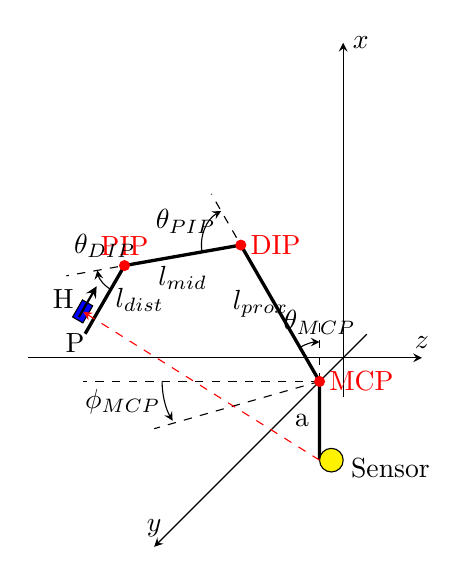
\begin{tikzpicture}[x=0.5cm,y=0.5cm,z=0.3cm,>=stealth]
% coordinate system axes
\draw[->] (xyz cs:x=-8) -- (xyz cs:x= 2) node[above] {$z$};
\draw[->] (xyz cs:y=-1) -- (xyz cs:y= 8) node[right] {$x$};
\draw[->] (xyz cs:z= 1) -- (xyz cs:z=-8) node[above] {$y$};
% the finger
\newcommand\offx{-1}

\coordinate (O) at (0,0,\offx);
\coordinate (S) at (0,-2,\offx);
\coordinate (O-) at (0,1.5,0);
\coordinate (off) at (0,0,-2);
\coordinate (MCP) at (120:4);
\coordinate (MCP-) at (120:1.5);
\coordinate (DIP) at (190:3);
\coordinate (DIP-) at (190:1.5);
\coordinate (PIP) at (240:2);
\coordinate (PIP-) at (240:1.5);
\coordinate (P) at (234:1.8);
\coordinate (T) at (149.5:5.78);	% not a good solution...

% lines, representing the phalanges
\draw[dashed] (O) -- ++ (MCP) -- ++(MCP-);
\draw[dashed] (O) -- ++ (O-);
\draw[black,very thick] (S) -- node[left] {a} (O) -- node[below,pos=0.75]{$ l_{prox} $} ++ (MCP) -- node[below]{$ l_{mid} $} ++ (DIP) -- node[right]{$ l_{dist} $} ++ (PIP);
\draw[dashed] (O) -- ++(MCP) -- ++ (DIP) -- ++(DIP-);
\draw[dashed] (O) -- ++(-6,0,0);
\draw[dashed] (O) -- ++(-3,0,-2);

% the red dots for the joints
\fill[red] (O) circle(2pt) node[right] {MCP};
\fill[red] (O) ++ (MCP) circle(2pt) node[right] {DIP};
\fill[red] (O) ++ (MCP) ++ (DIP) circle(2pt) node[above] {PIP};

% the angles
%\draw[<-] ((0,1,0)) arc (-270:-240:1);
%($(<center>) + (<init angle>:<radius>)$)
\draw[<-] ($(O)+(-270:1)$) arc (-270:-240:1);
\path (O)+(90:1.5) node {$\theta_{MCP}$};
\draw[<-] ($(O)+(MCP)+(-240:1)$) arc (-240:-170:1);
\path (O)++(MCP)+(-1.4,0.6,0) node {$ \theta_{PIP} $};
%\draw[<-] ([shift={(-170:0.7)}] T) arc (-170:-120:0.7);
\draw[<-] ($(O)+(MCP)+(DIP)+(-170:0.7)$) arc (-170:-120:0.7);
\path (O)++(MCP)++(DIP)+(-0.5,0.5,0) node {$ \theta_{DIP} $};
\draw[->] ($(O)+(-4,0,0)$) arc(-180:-150:2);
\path (O)++(-4,0,0)+(-1.0,-0.5,0) node{$ \phi_{MCP} $};
%

% the magnet
\draw[fill=blue,rotate=240+180,shift={($(O) + (MCP) + (DIP) + (P)$)}] (0,0,0) rectangle(0.5,0.3,0);
\draw[black,thick,->] ($(O) + (MCP) + (DIP) + (P) + (-0.1,0.15,0)$) -- ++ (240+180:0.9);
\path (O) ++ (MCP) ++ (DIP) ++ (P) + (-0.5,0.6,0) node (H) {H};
\path (O) ++ (MCP) ++ (DIP) ++ (P) + (-0.2,-0.5,0) node (P) {P};

\draw[fill=yellow,rotate=90,shift={($(S)$)}] (0,-0.3,0) circle(0.3);
\path (S) + (1.8,-0.2,0) node {Sensor};

% vector R
\draw[dashed, red, ->] (S) -- ++ (H);

\end{tikzpicture}
\caption{Kinematic chain for representation of a single finger. The cartesian coordinate system is aligned according to the sensor frame. This coordinate system defines the orientation, used throughout the whole thesis. The \ac{MCP} joint lies on the y-Axis. \todo{split it!}}
\label{fig:handMod}
\end{figure}
For the calculation of the magnetic flux density according to the models, introduced in \ref{sec:magneticFound}, the distance vector from sensor to magnet and the orientation of the latter one is needed. Those two components can be derived using forward kinematics and the positions of the sensors and the joints.\\
The orientation vector $ \vec{h} $ is derived in the following way:
\begin{equation}\label{eq:orienH}
\begin{aligned}
h_{x} =& \cos(-\theta_{MCP}-\theta_{PIP}-\theta_{DIP})\\[3pt]
h_{y} =& \cos(-\theta_{MCP}-\theta_{PIP}-\theta_{DIP})\sin(\phi)\\[3pt]
h_{z} =& \sin(-\theta_{MCP}-\theta_{PIP}-\theta_{DIP})\cos(\phi)
\end{aligned}
\end{equation}

The position vector $ \vec{r} $ of the magnet is determined by
\begin{equation}\label{eq:posX}
\begin{aligned}
r_{x} =& l_{Prox}\sin(\frac{\pi}{2}-\theta_{MCP}) +\\
& l_{Mid}\sin(\frac{\pi}{2}-(\theta_{MCP}+\theta_{PIP})) +\\
& l_{Dist}\sin(\frac{\pi}{2}-(\theta_{MCP}+\theta_{PIP}+\theta_{DIP})) + (P_{MCP_{x}} - P_{Sensor_{x}}) \\[4pt]
r_{y} =& l_{Prox}\cos(\frac{\pi}{2}-\theta_{MCP}) +\\
& l_{Mid}\cos(\frac{\pi}{2}-(\theta_{MCP}+\theta_{PIP})) +\\
& l_{Dist}\cos(\frac{\pi}{2}-(\theta_{MCP}+\theta_{PIP}+\theta_{DIP}))\sin(\phi) + (P_{MCP_{y}} - P_{Sensor_{y}}) \\[4pt]
r_{z} =& -l_{Prox}\cos(\frac{\pi}{2}-\theta_{MCP}) +\\
& l_{Mid}\cos(\frac{\pi}{2}-(\theta_{MCP}+\theta_{PIP})) +\\
& l_{Dist}\cos(\frac{\pi}{2}-(\theta_{MCP}+\theta_{PIP}+\theta_{DIP}))\cos(\phi) +(P_{MCP_{z}} - P_{Sensor_{z}})
\end{aligned}
\end{equation}
with $ l_{Prox}, l_{Inter}, l_{Dist} $ being the bone lengths of the associated phalanges, $ P_{MCP} $ the position of the \ac{MCP} joint and $ P_{Sensor} $ the position of the sensor. Those hand dimension parameters are very important, since they define the expectable $ \vec{r} $ and have therefore an influence for calculating the expected magnetic flux densities. Remember, that $ \vec{r} $ contributes nonlinearly to the magnetic models and therefore to the expected flux density. They should be determined very exact, to get a right representation of the proband, wearing the system. However they can only be measured up to a certain grade of accuracy, since the bones and joints lie underneath the skin. An x-ray could provide exact anatomic values, but this would seem to break the range of effort. Therefore in the end a calliper is used for identifying the anatomic bone lengths and the sensor and joint positions of the hand. As mentioned, this has to be done very accurate to get a detailed representation of the fingers. For neglecting the adduction-abduction movement, one just has to set the $ \phi $ value to 0. From that it directly follows, that the orientation and position vectors have only contributions on the $ x $- and $ z $-axis. The $ y $-component stays 0.\\
Summarizing the derived hand model, one can define the state space of one finger pose to be totally described by 3 angular values (for the version neglecting adduction-abduction, the state space reduces to 2), being
\begin{equation*}
\begin{aligned}
x &= \begin{bmatrix}
				\theta_{MCP}\\
				\theta_{PIP}\\
				\phi_{MCP}
\end{bmatrix}
\end{aligned}
\end{equation*}
This state vector is further also refereed as the finger state vector. Thus all four fingers have a state space of size 12. The presented model shows a basic approach to model the index, middle, ring and pinky finger of the human hand as ideal revolute joints. The constraints and simplifications introduced are comparable to other groups \cite{lin2000modeling}. The biggest simplification however is the disregard of the thumb movement.



\section{Sensor Design and Data Acquisition} \label{cha:sensors}

For measuring the magnetic field, four LSM303D sensors \cite{STlsm2012} from ST are used. This device comprises a 3 axis accelerometer and a 3 axis magnetometer in one module. This sensor is chosen, because its magnetic full-scale range is selectable. It can be determined to $ \pm 0.2$, $ \pm 0.4 $, $ \pm 0.8 $ or $ \pm 1.2\si{\milli\tesla} $. The magnetic values are stored in 2 Bytes in 2's complement. The sensitivity per \ac{LSB} is specified like shown in \ref{tab:magSensitivity}.
\begin{table}[h]
\centering
\begin{tabular}{c|l}
%\hline
\textbf{Measurement Range [\SI{}{\milli\tesla}]} & \textbf{Sensitivity [\SI{}{\micro\tesla \per LSB}]} \\ \hline
$ \pm 0.2 $ & 0.080 \\ \hline
$ \pm 0.4 $ & 0.160 \\ \hline
$ \pm 0.8 $ & 0.320 \\ \hline
$ \pm 1.2 $ & 0.479 \\ %\hline
\end{tabular}
\caption[Magnetic sensitivity]{Magnetic sensitivity for the corresponding measurement range, according to the datasheet of the LSM303D sensor unit \cite{STlsm2012}.}
\label{tab:magSensitivity}
\end{table}
The data rate can be set to a maximium of \SI{100}{\Hz}. The communication is established via a standard I2C bus, which means that a clock frequency of \SI{100}{\kilo \Hz} is used. In the end a breakout version of this device, available from Pololu \cite{pol2016} is used. It is sold as a full 9 \ac{DOF} IMU, carrying the LSM303D and L3GD20H gyroscope. However since the gyroscope and the accelerometer are not further used, they won't be explained here in detail. A picture of the breakout board is shown in \ref{fig:breakout}. The communication is realised with an RFduino microcontroller. This device can be programmed via the Arduino environment, which eases the process. It comes with a built in \ac{BLE} module. This is used to send the data to a host PC, where the state estimation process is programmed. Since the same sensor is used four times on a single I2C bus, a small work around is established, to enable an individual communication to each one of the four sensors. The clock signal is splitted via a multiplexer and only redirected to the device, from which the data is desired. This ensures, that each sensor can be read out individually. Combining the data lines of the sensors and multiplexing the clock signal to each device individually leads to a single data information on the bus. As multiplexer, a breakout of the CD74HC4067 from Texas Instruments is used \cite{TImux2003}.
\begin{figure}
\centering
\includegraphics[width=0.2\textwidth]{pictures/LSM303breakout.jpg}
\caption[Breakout board of sensor unit]
{The utilized MinIMU-9 v3 breakout board from Pololu \cite{pol2016}}
\label{fig:breakout}
\end{figure}


\section{Calibration and Preprocessing of Sensor Data} \label{sec:caliPrepro}

\subsection{Calibration for Hard and Soft-Iron Coefficients} \label{subsec:hardSoft}

Magnetic sensors in general suffer from two main distortion effects, being the hard and soft-iron coefficients. Those parameters are caused by manufacturing processes, ferromagnetic materials on the \ac{PCB} and the immediate environment of the sensor \cite{ozyagcilar2012calibrating}. If the device is moved in a field, free of artificial magnetic distortion, it should only measure the influence due to the earth's magnetic field. An ideal device would measure a constant value for the field strength, no matter in which way it is oriented. In other words, holding the device, such that the full earth field has only influence on the $ z $-axis, should provide the same result on the other axes, when rotating it to the corresponding one. So in the end by measuring the earth magnetic field at various positions and plotting them, should result in a perfect sphere, centered at the origin. Due to the hard iron distortions the sphere is not perfectly located at the center. This effect is produced by materials, exhibiting a constant additive field, like wires or small ferromagnetic components, placed onto the \ac{PCB} \cite{konv2009}. Soft iron effects however, cause that the shape of the sphere is deformed to an ellipsoid. The are induced by materials, influencing the pervasion of magnetic field lines and causing different gains on the axes. An example would be metallic materials like iron or nickel, which influence the direction of magnetic fields. So in the end the shape of the expected sphere is more like an ellipsoid, shifted from the origin. A visualization can be seen in \ref{fig:hardSoft}.
\begin{figure}
\centering
\includegraphics[width=0.7\textwidth]{pictures/hardSoft.png}
\caption[Calibrated and uncalibrated sensor data]
{The plot shows the obtained sensor values for the earth magnetic field, by moving the sensor in space. The ellipsoid on the right side shows the influence of hard and soft-iron distortion coefficient. The red dots represent the uncalibrated measurements. The sphere around the blue dots on the left displays the calibrated, perfect sensor values \cite{ozyagcilar2012calibrating}.}
\label{fig:hardSoft}
\end{figure}
The static hard-iron effects can simply be modelled as an offset $ H $, shifting the magnetic values. The soft-iron effects are represented by a $ 3\times3 $ matrix $ W $, transforming the sphere into an ellipsoid. So in order to describe the measurement of a sensor in absence of artificial magnets, one could utilize the following model for the magnetic flux density of the earth:
\begin{equation} \label{eq:hardSoftModel}
\mathrm{B}_{earth} = W^{-1} (\mathrm{B}_{meas} - H)
\end{equation}
To determine and overcome these two distortion factors, several methods exist. For a naive approach, the offset parameters $ H $ are simple to determine. One takes the average between the maximum and minimum of one axis. \ref{eq:simpleOffset} shows this exemplary for the $ x $-axis.
\begin{equation} \label{eq:simpleOffset}
\mathrm{off}_{x} = \frac{x_{max} + abs(x_{min})}{2}
\end{equation}
The 6 soft-iron parameters can be specified, by performing an ellipsoid fit. Kok et al. follow a very elaborated approach, by applying an elliptical fit in combination with measurements of inertial sensors. This approach also covers the alignment of the sensor axes of the magnetometer with the ones of the gyroscope and accelerometer. Since only the magnetic sensor is used for the further experiments, this can be neglected. The Application Note 4246 by Freescale \cite{ozyagcilar2012calibrating} presents a good and interesting calibration procedure. They reduce the determination of the three hard- and the nine soft-iron factors to four parameters. This is utilized, by assuming that the hard-iron offsets dominate the soft-iron effects and one is trying to minimize the error between the measured field $ \mathrm{B}_{meas} $ and the real, surrounding field $ \mathrm{B}_{earth} $. For this, they take a whole series of measurements into account, and not just the minimum and maximum, like for the naive approach in \ref{eq:simpleOffset}. As a result, one gets a vector with the three offset values $ H $ and the flux density of $ \mathrm{B}_{earth} $. However, by using the more naive approach and the assumption that the soft iron values do have an influence on the measurements, one could perform a simple compensation of those. One models the influence of the soft iron distortion as a one dimensional vector, increasing or decreasing the overall measured field of one axis. For this, the average amounts of the obtained magnetic field, representing the \grqq radius \grqq of each axis are determined. Those three values are averaged, to perform the overall radius $ \mathrm{rad}_{avg} $. \ref{eq:simpleScale} show how to derive this scaling factor for the $ x $-axis.
\begin{equation} \label{eq:simpleScale}
\begin{aligned}
\mathrm{rad}_{x} &= \frac{x_{max} - x_{min}}{2}\\
\mathrm{rad}_{avg} &= \frac{\mathrm{rad}_{x} + \mathrm{rad}_{y} + \mathrm{rad}_{z}}{3}\\
\mathrm{scale}_{x} &= \frac{\mathrm{rad}_{avg}}{rad_{x}}
\end{aligned}
\end{equation}
In the end, independent on how the sensors get calibrated, one has to do this routine for each sensor to get the individual parameters. Due to the performed calibration procedure, the measurement range of the sensor is slightly varied. As an additional step, the sensors have to be scaled to the same measurement range. By calibrating the sensors with the Freescale method, one directly gets a value for the surrounding field. It turns out, that these values are not equal for different sensors, such that each device has slightly another sensitivity. So one has to determine a scale factor, to bring the sensors onto the same measurement range.


%\subsection{Fitting the Sensor Data to the Model Equations} \label{subsec:modelFit}
%\todo{Write it a bit different!\\}
%Another preprocessing step concerning the measurements, is an additional adaptation of the observed sensor values to the model equations. After the calibration phase, it can happen, that on the one hand the sensor readings are calibrated and show all the same measurement range, but on the other hand, those values have to be set in relation to the actual model equations, to represent the de-facto magnetic flux density. In other words, the calibration of the sensors is improved through this step. The difference between the model and the observable sensor values comes also from the scaling to a common value for the earth magnetic field. No normed sensor was at hand to determine the real earth magnetic field at the calibration position at the lab, therefore just one value was chosen, to fit all sensors to. Further on the presented calibration procedures are not totally fault-free. The scaling factors are expected to be small. For this step, a rigid, non metallic construction would be ideal. However this was not available. In return an almost accurate fitting procedure is evaluated.
%
%The calibrated sensors are placed inside the rack and attached onto a small box. A magnet with known characteristics is moved on a predefined path with fixed orientation in front of them. The set up and the movement should result into a three dimensional influence for all sensors. By holding and moving the magnet, the distance vector $ \vec{r} $ and the orientation is known. So the values for the magnetic field can be estimated for each sensor. Those serve as a ground truth for the scaling of the sensor data. In \ref{fig:caliFlat} a picture of the set up is shown. Since this procedure is performed on a normal table, with self determined position and orientation parameters and done \grqq by-hand \grqq, this process is fault prone. However it should still be possible to verify the calibration procedure and push the sensor data towards the predictions of the model equations.
%
%\todo{Describe it more!!! Say that the hand parameters cannot be determined good enough blablabla\\}
%Another calibration method would be the introduction of an initialization gesture on the hand. Beforehand the dimensions on the hand and the sensor and finger positions have to be measured. The gesture consists of bending all four \ac{MCP} joints simultaneously around \SI{90}{\degree}. To make this process reproducible, the gesture should be performed along a rectangular piece of cardboard (Pictures are provided at \todo{find/make pictures!} \ref{fig:caliHand}). Again this movement can easily be simulated by the model equations and the measurements can be fitted to them. For this approach, the exact determination of the hand dimensions is critical, since they play a fundamental role in the calculation of the position vector $ \vec{r} $ for the magnetic field models (see \ref{eq:posX}). Those values comprise the lengths of each bone, the sensor and joint positions. A fit to a wrong set of localizations and dimensions would lead to wrong predicted magnetic flux densities and could degrade the results of the pose estimation. Since it is not possible to determine those parameters exactly by hand, and since they vary slightly by movement, those scaling factors are expected to fluctuate within various measurement sets. However this method represents an application driven fitting procedure and will probably lead to better results for the pose estimation, what is the overall aim of the system. Since the scaling values slightly change with the movement and placement of the sensor rack on the hand and by the provided hand parameters, those values have to be defined each time.
%\begin{figure}[h]
%\centering
%\includegraphics[width=0.6\textwidth]{pictures/caliFlat1.JPG}
%\caption{Setup for easy calibration on table. The magnet is moved on a predefined path along the arrows. \todo{insert arrows and coordinate frame! Add a picture with straigth and 90 orientation of hand}}
%% for this look at http://tex.stackexchange.com/questions/198492/how-can-i-annotate-a-figure-with-lines-and-circled-numbers
%% or just google for "latex anotate figure"
%\label{fig:caliFlat}
%\end{figure}

\subsection{Cancellation of the Surrounding Earth Magnetic Field} \label{subsec:earthEli}

The magnetic models, introduced in \ref{sec:magneticFound} describe the influence of the magnets at a certain position and orientation, relative to the sensor. Another observation proven in that chapter is that multiple magnetic fields sum up. On earth we focus a static surrounding magnetic field, going from the south pole to the north pole. Depending on the position at the planet, this value ranges from 25 - \SI{65}{\micro \tesla}. This field cannot easily be shut down and automatically contributes to the sensor measurements. However for a proper interpretation of the surrounding field, solely determined by the permanent magnets, the earth field has to be eliminated. For a system with static geological sensor position and orientation, this would be easy. One would just measure the field without any artificial magnets and subtract this from every ongoing measurement. Obviously, the geological position and orientation of the human hand during normal tasks is naturally not static.\\
By knowing the orientation of the system and the corresponding earth magnetic field in absence of artificial magnets, it should be possible, to eliminate this offset. The following cancellation process is utilized, to get the earth magnetic field, relative to the sensor position:\\
\begin{enumerate}
\item Hold the hand with the sensors attached in a stable and calm position
\item The magnets for the fingertips are absent
\item Measure the orientation $ R_{I} $ of the sensors and the corresponding surrounding earth magnetic field $ \mathrm{B}_{earth} $
\item After this calibration phase, one tracks the orientation of the hand $ R_{h} $
\item Calculate the relative orientation $ R_{d} = R_{I} - R_{h} $
\item Convert $ R_{d} $ into a rotation matrix $ rot_{d} $ and apply this to $ \mathrm{B}_{earth} $
\item Subtract the rotated earth magnetic field from your actual measurement, s.t. \\ $ \mathrm{B} = \mathrm{B}_{meas} - rot_{d} \cdot \mathrm{B}_{earth} $
\end{enumerate}
As stated in \ref{cha:sensors} the used sensor breakout comes with a full 9 \ac{DOF} \ac{IMU}. With such a system the orientation can be estimated. The Madgwick filter \cite{madgwick2010efficient} is a widely used method for deriving the absolute orientation of a body in space, by using gyroscope, accelerometer and magnetometer data. However this estimation uses the earth magnetic field, to compensate sensor drifts and to align its orientation, relative to it. So by introducing artificial magnets, which are stronger than the earth magnetic field, the Madgwick filter could break down and therefore the calculated orientation can drift. In \ref{subsec:resEarthEli} the evaluation of this approach is shown. 


\section{Magnetic Field Interpretation Towards Finger Pose Reconstruction} \label{sec:magmodel}

For the following section it is important to note, that the Cartesian coordinate system, introduced in \ref{sec:handModel} and visualized in \ref{fig:handMod} is applied. It represents the orientation of the sensor frame, which is assumed to be static. The following two sections show how to calculate the three dimensional magnetic field value $ \mathrm{B}(x) $ for the finger state vector $ x $. As mentioned in \ref{sec:handModel}, the position of the sensors $ P_{sensor} $, the lengths of the phalanges and the static positions of the \ac{MCP} joints $ P_{MCP} $ have to measured very exactly, to get a proper value for the expectable magnetic flux density for a certain finger pose. 

For describing a magnetic flux density with the dipole model (\ref{eq:dipole}), introduced in \ref{sec:magneticFound}, one has to define the vectors $ \vec{r} $ and $ \vec{h} $ accordingly. The derivation of those two, according to the kinematic chain is described in \ref{sec:handModel} (see \ref{eq:orienX} and \ref{eq:posZ}).
For describing the magnetic flux density of a certain finger state with the cylindrical bar magnet model some further adjustments have to be done. Since the model uses cylindrical coordinates ($ z, \rho, \varphi $), the Cartesian ($ x, y, z $) of the sensor and magnet positions have to be transformed. One also has to note, that the values, calculated by this model assume, that sensor and magnet are aligned equally (I want to say in the same coordinate frame/pointing into the same direction???). Since the magnet is rotating around the $ y $- (by flexion-extension) and $ z $-axis (by adduction-abduction) and the sensor keeps its static orientation on the back of the hand, the alignment of the two parts changes. To overcome this rotation, the Cartesian values of the distance vector $ \vec{r} $ have to be rotated about the orientation of the magnet. The following formulas describe the required rotation and transformation adjustments:
\begin{equation}
\begin{aligned}
\vec{r}_{rot} &= rot_{y}(\theta_{MCP} + \frac{5}{3} \theta_{PIP}) \cdot rot_{z}(\phi) \cdot \vec{r}\\[3pt]
z &= \vec{r}_{rot}[0]\\
\rho &= \sqrt{\vec{r}_{rot}[1]^{2} + \vec{r}_{rot}[2]^2}\\
\varphi &= \arctan(\vec{r}_{rot}[1], \vec{r}_{rot}[2])
\end{aligned}
\end{equation}
The transformation from calculated cylindrical components of the magnetic flux density back to Cartesian is done by
\begin{equation}
\begin{aligned}
\mathrm{B}_{x_{rot}} &= \mathrm{B}_{z}\\
\mathrm{B}_{y_{rot}} &= \mathrm{B}_{\rho}sin(\varphi)\\
\mathrm{B}_{z_{rot}} &= \mathrm{B}_{\rho}cos(\varphi)\\[3pt]
\mathrm{B} &= (rot_{y}(\theta_{MCP} + \frac{5}{3} \theta_{PIP}) \cdot rot_{z}(\phi))^{-1} \cdot \mathrm{B}_{rot}
\end{aligned}
\end{equation}
As already depicted in \ref{sec:magneticFound}, the exact solution of a \ac{CEL} is hard to calculate. Bulirsch et al. \cite{bulirsch1965numerical} describe some approaches in their work to approximate the result. They extended ideas of Landen and Gauss for the solution. The used calculation algorithm, is given in \cite{derby2010cylindrical}, a version in pseudocode is provided in the \todo{Appendix}. Like other numerical methods it uses a loop, to terminate at a certain accuracy level. This brings in, that the function can not further be treated as a natural equation, when it comes to further differentiation.



\section{Hand State Estimation} \label{sec:estimation}

Assumed is a system with $ K $ magnets and $ N $ sensors. The beforehand models for deriving the magnetic flux density are refereed equally as $ \mathrm{B}_{n}(x_{k}) $ representing the field at sensor $ n $, excited by the finger state vector $ x_{k} $ of magnet $ k $. Since magnetic fields sum up, for $ K > 1 $, this is a cumulative sum over all the presented magnets $ k $, being
\begin{equation}
\mathrm{B}_{n} = \sum_{k=1}^{K} \mathrm{B}_n(x_{k})
\end{equation}
for sensor $ n $. Since the state $ x_{k} $ consists of 3 values, the complete system state vector has a shape of $ (3 \cdot K) \times 1 $ and is denoted by
\begin{equation}
\begin{aligned}
& \mathrm{X}_K &= \begin{bmatrix} x_{1} & x_{2} & \cdots & x_{K}  \end{bmatrix}^{T}\\
&  &= \begin{bmatrix} \theta_{MCP_{1}} & \theta_{PIP_{1}} & \phi_{MCP_{1}} & \theta_{MCP_{2}} & \cdots \end{bmatrix}^{T}
\end{aligned}
\end{equation}
the overall measurable magnetic flux densities corresponding to a system state $ \mathrm{X}_{k} $ by the $ N $ sensor units is 
\begin{equation}
\begin{aligned}
\mathrm{M} &\equiv \begin{bmatrix} {\mathrm{B}}_{1} & {\mathrm{B}}_{2} & \cdots & {\mathrm{B}}_{N} \end{bmatrix}^{T}\\
		&= \begin{bmatrix}
			\sum_{k=1}^{K} \mathrm{B}_1(x_{k})\\
			\sum_{k=1}^{K} \mathrm{B}_2(x_{k})\\
			\vdots \\
		    \sum_{k=1}^{K} \mathrm{B}_N(x_{k})\\
		\end{bmatrix} \\
	    &= \mathrm{M}(\mathrm{X}_K)
\end{aligned}
\end{equation}
The measurement of sensor $ n $ is denoted by $ \tilde{\mathrm{B}}_{n} $, the measurement array of all sensors $ N $ has a shape of $ (3 \cdot N) \times 1 $ and is represented by
\begin{equation}
\begin{aligned}
& \tilde{\mathrm{M}} \equiv \begin{bmatrix} \tilde{\mathrm{B}_{1}} & \tilde{\mathrm{B}_{2}} & \cdots & \tilde{\mathrm{B}_{N}} \end{bmatrix}^{T}\\
& \text{with: }  \tilde{\mathrm{B}}_{n} = \begin{bmatrix} \tilde{\mathrm{B}}_{n}(x) & \tilde{\mathrm{B}}_{n}(y) & \tilde{\mathrm{B}}_{n}(z) \end{bmatrix}
\end{aligned}
\end{equation}
In order to derive an estimate of the system state $ \mathrm{X}_K $, one can formulate an optimization problem. The objective function $ f(\mathrm{X}_K) $ for the minimization of the residual between the actual sensor measurements and the state representation by the model is described by:
\begin{equation} \label{eq:minimization}
\begin{aligned}
\underset{\mathrm{X}_K}{\text{minimize}} & & f(\mathrm{X}_K) = || \tilde{\mathrm{M}} - \mathrm{M}(\mathrm{X}_K) ||\\
\text{subject to} & & 0 & \leq {x}_1(\theta_{MCP}) \leq & 1/2 \cdot \pi, \\
				  & & 0 & \leq {x}_1(\theta_{PIP})  \leq & 110/180 \cdot \pi, \\
				  & & -30/180 \cdot \pi & \leq {x}_1(\phi_{MCP}) \leq & 30/180 \cdot \pi, \\
				  & & 0 & \leq {x}_2(\theta_{MCP})  \leq & 1/2 \cdot \pi, \\
				  & & \vdots \\
				  & & -30/180 \cdot \pi & \leq {x}_K(\phi_{MCP}) \leq & 30/180 \cdot \pi
\end{aligned}
\end{equation}
As constraints, the natural range of motion for each finger angle is utilized. The solvability and the uniquness of the result for this minimization is dependent on the determinedness of the system. To gather unique and clear solutions, the system has to be fully determined at any time. Since one is trying to estimate the pose of 4 magnets, by also using 4 sensors, this condition is fulfilled. For minimizing such a function, one has to remember the mathematical form of the introduced magnetic models. The dipole model includes nonlinearities, the cylindrical model in contrary is solved by a numerical approximation, which in return means that differentiation or further mathematical operations can not be applied. Since the programming language \emph{Python} \cite{python} is used to solve this problem, it is refereed to methods provided by the \emph{SciPy} \cite{scipy} package . This library provides a minimize method, that is implemented just for such use cases. It comes with several user definable options, to provide the solver with additional information. In \ref{subsubsec:resSim} the utilized optimization methods are explained and the performance and quantity of the results are compared. Anyway, to speed up the computational time for solving the equations and the optimization problem, the functions are implemented in Cython \ref{cython}. This interface allows to write C-like Python code and to work with predefined variables. 

%Another way of solving such a state estimation problem is by applying a Kalman Filter. This filter comprises a prediction step, foreseeing the next system state and an update step, correcting this prediction with the actual measurements. The utilized recursive filter equations are described by
%
%\emph{Prediction step:}
%\begin{equation}
%\begin{aligned}
%\hat{\mathrm{X}}_{K}(t) &= \mathrm{X}_{K}(t-1)\\
%P(t) &= P(t-1) + Q
%\end{aligned}
%\end{equation}
%\emph{Update step:}
%\begin{equation}
%\begin{aligned}[l|l]
%G &= \frac{P(t) J_{\mathrm{M}}}{(J_{\mathrm{M}} P(t) J_{\mathrm{M}}^{T} + R)} \\
%\hat{\mathrm{X}}_{K}(t+1) &= \mathrm{X}_{K}(t) + G[\tilde{\mathrm{M}} - \mathrm{M}(\hat{\mathrm{X}}_{K}(t))]\\
%P(t+1) &= (I - G J_{\mathrm{M}}) P(t)
%\end{aligned}
%\end{equation}
%As one can see, some simplifications have been applied to the \ac{EKF}. A state transition model, describing the behaviour of the system between two measurements, is left out. This assumption is made, because the intention of the user and therefore the evolution of the state is not known. So the predicted system state is assumed to stay constant. The process noise matrix $ Q $ and the measurement noise $ R $ are assumed to be diagonal matrices. This can be said, since the measurements of each axis and sensor do not effect each other. Nonetheless, it would be possible to bring in inter finger constraints by a $ Q $ matrix, showing contributions on the off-diagonals. Since those restrictions can not be generalized for every human hand, they are left out. The \ac{EKF} uses the Jacobian of the model, to linearize around the actual predicted state. This is denoted by
%\begin{equation}
%J_{M} = \left . \frac{\partial \mathrm{M}}{\partial \mathrm{X}} \right \vert _{\hat{\mathrm{X}}_{K}(t)}
%\end{equation}
%This method is computationally fast, since only matrix calculations have to be performed. Casually spoken, the $ Q $ matrix gives a measure how much the system state will change. By introducing big values, the state is assumed to change much, vice versa for small values. Via $ R $ it can be determined, how much one can trust the obtained sensor values. Small entries assume to have exact measurement data, big values the contrary. By adjusting those two matrices, one can tune the filter equations and therefore the result. One drawback of this method is, that it cannot be constrained.





\section{Visualization} \label{sec:visual}

Another part of the system is the visualization of the estimated state. On the one hand, the values could be displayed with a graph. This way is very good, to get an accurate insight in the outcome of the estimation phase and for comparing it to ground truth data or similar state sets. However this approach is not very intuitive and for untrained\todo{(unskilled/people how know about the state estimation background...)} people, like patients of a clinical study not very helpful. For this, an application with the Blender Game Engine \cite{blender} is implemented, displaying a 3D human hand. The utilized hand model already provides a rig, representing the bone structure. This eases the further manipulation and setting of the corresponding finger angles. The bending of a joint can be modelled by rotating the corresponding points of the model. Blender provides a Python programming interface, for modifying and animating 3D models. The underlying script, changing the orientation of bones, concentrates on the very basics for representing the state. For communicating with the state estimation script, a simple text file is used. The real time state estimation writes its values each time at the very beginning of the file. This ensures, to keep additional disk space on the executing system small, since only $ 3 \times K $ float values are written each step. The Blender Game is situated in a loop, constantly reading the first line of this file. To ensure transmission security, one has to note that the estimation phase should only be allowed to write complete lines, describing the whole actual state. Some screenshots of the application are provided in \ref{fig:blendGame}

\begin{figure}[h]
\centering
	\subfloat[Fingers in stretched position]
	{\includegraphics[width=0.5\textwidth]{pictures/game2.png}\label{fig:gameStretch}}
	\hfill
	\subfloat[Fingers in crooked position]
	{\includegraphics[width=0.5\textwidth]{pictures/game1.png}\label{fig:gameCrooked}}
\caption{Screenshots of the visual representation with Blender}
\label{fig:blendGame}
\end{figure}


\lhead[\chaptername~\thechapter]{\rightmark}

\rhead[\leftmark]{}

\lfoot[\thepage]{}

\cfoot{}

\rfoot[]{\thepage}

\chapter{Results} \label{cha:results}

\section{Sensor Behaviour} \label{sec:dataRes}

The utilized LSM303D sensors show some general measurement characteristics. If they are exposed to a magnetic field, higher than the configured measurement range, a clipping of the returned value can be observed. In \ref{fig:clipping} this effect can be seen on the observed values along the magnetic $ x $-axis. The magnet is moved along this axis towards the sensor. As expected, the measured field increases/decreases, by shrinking the distance $ \Delta d $ between sensor and magnet. Looking at \ref{fig:negClip}, approximately at a distance of \SI{4.5}{\cm} between sensor and magnet, the measured field reaches the current lower range. The sensor first stays a while on this value, before it jumps to positive. By turning the magnet around \SI{180}{\degree} and therefore measuring an increasing magnetic field by the sensor, a similar behaviour can be recognized. This time the clipping obviously occurs from positive to negative and happens at a gap of \SI{4}{\cm} (see \ref{fig:posClip}). Further on, this time the returned value clips directly and does not stay on a maximum value. To overcome this effect, one has to set the magnetic full scale range to an appropriate value. However by setting for every user the maximum range of $ \pm \SI{1.2}{\milli \tesla} $, one looses precision in the measurements. The approximately reachable maximum full scale range for one user can easily be determined. By simulating the range of possible flexion-extension, which would be performing a fist, and looking at the predicted outcome of the  model, one gets an image for the result of the measurable magnetic field. From that the measurement range can be determined. However due to the influence of surrounding magnetic fields, this value is only a guideline for the de facto measured field. Based on this context, the magnetic full scale range of the sensors for the ongoing measurements and experiments is set to $ \pm \SI{0.4}{\milli \tesla} $.

\begin{figure}[!htb]
\subfloat[Moving the negative pole towards the sensor]
{\includegraphics{pictures/plots/negClipping.png} \label{fig:negClip}}
\hfill
\subfloat[Moving the positive pole towards the sensor]
{\includegraphics{pictures/plots/posClipping.png} \label{fig:posClip}}
\caption[Clipping behaviour of sensor]
{The magnet is moved towards the measurement unit, to record the clipping behaviour of the sensors. The distance from sensor to magnet is represented by $ \Delta d $ in \si{\cm}. For \label{fig:negClip}, the oversteering of the sensor begins at around \SI{4.5}{\cm}, for \label{fig:posClip}, this effect starts at \SI{4}{\cm}. The sensor range is adjusted to be $ \pm \SI{0.4}{\milli \tesla} $, which can be observed by the dataplots.}
\label{fig:clipping}
%python script: 160214_clippingDetection.py
\end{figure}
For evaluating the timing behaviour of the system, the code on the RFduino is debugged. As described in \ref{cha:sensors}, the sensor data rate could be set to a maximum value of \SI{100}{\Hz}, such that one could retrieve new magnetometer values each \SI{10}{\milli \second}. The switching and forwarding of the clock signal via the utilized multiplexer takes only \SI{21}{\nano \second} into account. This value composes a \grqq Break-before-make\grqq \, pause of \SI{6}{\nano \second}, to prevent crosstalk between the channels and a propagation delay time of \SI{15}{\nano \second}. In order to verify those values and to identify the overall time for acquiring, scaling to distortion factors, sending and receiving the measurement data by the host system, the respective code sections were timed. It is observed that the overall sampling frequency of the sensors can only be set to \SI{50}{\Hz}. So the time between two new sensor read outs is \SI{20}{\milli \second}. The read out of the registers and the scaling for the hard- and soft-iron distortion values shows an insignificant influence on the timing. Further on it makes no difference whether only one sensor unit is read out, or all four, since they all show the same data rate and have measurements available after \SI{20}{\milli \second}.\\
The sending via BLE is implemented by the RFduino environment. The maximum transferable packet size is 20 bytes \cite{rfduino2015data}. The three float values of one sensor, plus an additional float for indicating the device number have a size of 16 bytes. The RFduino has implemented a queue of size 20 bytes, where the data is stored, till it is sent. The sending frequency depends on the distance between the host PC (which represents the client) and the RFduino module (which is the server). It is specified to range from \SI[per-mode=symbol]{32}{\kilo \bit \per \second} to \SI[per-mode=symbol]{24}{\kilo \bit \per \second}. In order to ensure that no data packet is overwritten, before it is sent, one has to check the size of the queue each time before writing to it. The client registers via the \ac{GATT} protocol for listening to the notifications of the microcontroller. For the ongoing interpretation of the sensor values, only measurements from all four units are interesting. Therefore, for identifying the overall data rate, the time for receiving four individual data packets from the server is measured. It is observed, that the receiving rate is not constant. For a sensor rate of \SI{50}{\Hz} it is observed, that approximately every \SI{50}{\ms} four new packets are received. This leads to a frequency of \SI{20}{\Hz} for the whole system. This high deviation from the actual possible sensor data rate is caused by the low sending frequency of the RFduino. Since the sensors are triggered with a frequency more than twice as high as the values can be received, their quality decreases. Therefore the data rate of the sensors is reduced to \SI{25}{\Hz}, in order to try to acquire more representative measurements. By doing this, the system frequency decreases to \SI{12.5}{\Hz}. However, this leads only to slightly more representative measurements, since the frequency for receiving the obtained data packets is still twice as high as the sensor data rate. Those results were observed, by measuring the acquisition time of 200 packets (each representing the measurements of four sensor units). The stated system frequencies represent the mean over the 200 observed timestamps. The histogram \ref{fig:sensTime}, represents the distribution of the measured duration for both sensor frequencies.
%\todo{Source of error for timing: The sending via BLE is time critical!... The RFduino safes the data into a queue. When you just put more and more data into this queue, while it is not sent (or without taking care whether the queue is full), you will overwrite entries! With checking the \grqq fullness \grqq of the queue with a while-loop (look at code!) you wait, till you are allowed to push the data to the queue. This ensures, that you don't overwrite entries. However your system is stuck during that time and since the sensor datarate with 50Hz is faster than the sending, data packets are lost! So you should try to adapt the sensor data rate to the sending rate. Taking one measurement out of 5(case with $ f_{sens} \gg f_{ble} $) is less good, than taking one out of 2(case for $ f_{sens} \geq f_{ble} $ ). This could lead to an overall slower acquisition of packets (since you have to wait longer for you sensors), but the values from the sensor are more representative!}
\begin{figure}[!htb]
\centering
\includegraphics{pictures/plots/timingRFd_v2.png}
\caption{200 acquisitions of complete measurement packets, comprising the values of four sensor units, where timed. One time the data rate of the sensor is set to \SI{50}{\Hz}, the other to \SI{25}{\Hz}. The mean value for $ f_{Sensor}=25\si{Hz} $ is higher than, for $ f_{Sensor}=50\si{Hz} $. However the variance of the acquisition time is smaller for this and therefore the outcome is more consistent to itself. Further on the sensor values from a data rate of \SI{25}{\Hz} represent the actual obtained measurements slightly better, than the higher data rate. In the ongoing evaluation, the results for both data rates are taken into account and compared to each other. \todo{smaller!}}
\label{fig:sensTime}
% python script: 160212_timing.py
\end{figure}


\section{Quality of Calibration Procedures} \label{sec:cali}

\subsection{Calibration for Hard and Soft-Iron Effects}\label{subsec:resHardSoft}

Two methods are compared and classified for determining the hard- and soft-iron factors. The naive approach, declaring the distortion values by using the maximum and minimum of the obtained measurements for an axis. This one is chosen, since it is an often cited and easy method for compensating the distortion factors. On the other hand, the version from Freescale \cite{ozyagcilar2012calibrating} which takes a whole series of measurements into account and only compensates for the hard-iron effects. 1000 measurements were collected, by rotating the sensor slowly around all possible axes. The environment is a normal lab, without any protections against additional, artificial magnetic fields. 

In \ref{fig:hs2d} the measurements for each axis combination are plotted in a two dimensional representation, for a clearer identification. The raw values are represented by the red dots, the calibrated by the green and cyan ones. The outline of the corresponding ideal sphere is visualized by the blue circle. It can easily be observed, that the hard iron effects dominate the soft iron factors. The scaling factors for the soft iron values, obtained by the naive approach also reflect this. They lie in the range of $ 1 \pm 0.03 $. Another fact is, that both calibration methods lead almost the same results. In order to compare the quality of the two calibration methods, the distance of each calibrated measurement value to the perfect sphere with radius $ \mathrm{B}_earth $ is calculated. The deviation is plotted as a histogram in \ref{fig:devi}. The obtained mean for the Freescale approach is calculated to be $ \mu_{Freescale} = -0.02\si{\milli \tesla} $, for the calibrated values, using the naive method to be $ \mu_{naive} = -0.8\si{\milli \tesla} $. So in the end the values calibrated by the Freescale approach represent slightly more the shape of a perfect centered sphere. One reason for this is, that for the utilized sensors the hard iron distortion effects dominate over the soft iron ones. Further on, since the whole measurement series is taken into account, the behaviour of the sensor is represented much better. The naive approach is very sensitive for noisy signals, since only the peak values characterize the calibration factors. One has to note, that those observations hold only for the used sensor units. For another \ac{PCB} environment or device, the obtained values could be different and the soft iron factors could show a higher influence. For this, the naive approach would probably lead to better results, than the Freescale. So in the end the calibration has to be verified and adjusted for the specific sensor and application.\\
The presented procedure was evaluated for several times and sensors, each time showing similar and constant results. As already mentioned in \ref{subsec:hardSoft} this calibration procedure has to be performed for each sensor and the observed values have to be additionally scaled to a common value for $ \mathrm{B}_{earth} $.
\begin{figure}[!htb]
\centering
	\subfloat[Obtained measurements along the $ x $ vs. the $ y $ axis]
	{\includegraphics{pictures/plots/cali_xy.png}\label{fig:xy}}
%	\hfill
	\subfloat[Obtained measurements along the $ y $ vs. the $ z $ axis]
	{\includegraphics{pictures/plots/cali_yz.png}\label{fig:yz}}
	\hfill
	\subfloat[Obtained measurements along the $ x $ vs. the $ z $ axis]
	{\includegraphics{pictures/plots/cali_xz.png}\label{fig:xz}}
\caption[2D representation of the raw calibration measurements]{
The measurements where recorded by rotating the sensor around each axis in an environment without artificial magnetic sources. 1000 measurements were collected. The obtained raw values are represented by the red dots. The results of the calibration procedures are plotted by the respectively color. The perfect centered sphere is represented by a circle with $ r=\mathrm{B}_{earth} $. Already the unscaled values show only a very low influence of soft iron distortion. It is also observed, that the calibrated results do not differ much. \todo{little bit smaller each}}
% python script: checkCalibration.py
\end{figure}
\begin{figure}[!htb]
\centering
\includegraphics{pictures/plots/cali_devi.png}
\caption[Deviation of the calibrated measurements to the perfect centered sphere]
{The procentual deviation of the two calibration methods to the corresponding perfect centered sphere is visualized. It can be obtained, that the Freescale approach leads to slightly more accurate results, since the mean and variance of the scaled measurements are smaller than for the naive approach.}
\label{fig:devi}
% python script: checkCalibration.py
\end{figure}
\todo{make statement about the range!}

%In \todo{3d} the calibrated and the uncalibrated data points are plotted, with a sphere around them. One thing that is clearly visible here is the shift, caused by the hard iron effects. In \todo{2d} this offset is also observable. Recognizable by those two plots is also the fact, that the influence of the soft-iron distortion is very small. The data points lie already on an almost perfect sphere. This is also represented in those scale values, calculated by the Winer approach. They lie in the range of $ 1 \pm 0.03 $. That both calibration methods serve almost the same results can already be seen by the fact that the blue and green datapoints are overlapping each other. In order to compare the two calibration methods, the distance of each calibrated value to the perfect sphere with radius $ \mathrm{B}_earth $ is calculated. The outcome is shown in \todo{deviation}. In the end, the mean value of the deviation for the Freescale approach is smaller than those, calibrated by the Winer method (for this particular example: $ \mu_{Freescale} = -0.0842\si{\micro \tesla}, \mu_{Winer} = 6.5525\si{\micro \tesla} $). Because the hard-iron offsets dominate the soft-iron effects, the Freescale method is more accurate than the Winer approach, since it takes all the observed measurements into account and not just the minimum and maximum values. Therefore for the utilized sensor units, which show small soft-iron deviation, the Freescale approach is preferred. The provided procedure was evaluated several times, each time showing similar and constant results. As already mentioned in \ref{subsec:hardSoft} this calibration procedure has to be performed for each sensor and the observed values all have to be scaled to a common value for $ \mathrm{B}_{earth} $.


%\subsection{Determining the Fitting Parameters for the Model} \label{subsec:resModelFit}
%
%\todo{Rewrite!}
%For determining the scaling factors to the model, the sensor rack is placed onto a cardboard box with a height of \SI{2}{\cm}. The magnet is statically aligned in the same direction as the sensor $ x $-axis and is moved along the y-axis on a flat surface. The distance in $ x $-direction is held static. The origin of the coordinate frame is determined to be the position of the upper most sensor unit. The magnet is moved at a distance of $ x=5\si{\cm} $ and $ x=7\si{\cm} $ from $ y=-6\si{\cm} $ (which is the $ y $-height of the under most sensor) to $ y=0\si{cm} $ (which is the $ y $-heigth of the upper most sensor). For defining the scaling factors, the B-field, which should be observed by the sensor is calculated. The range of the actually measured values is then fitted to the simulated ones for each axis. As a initial step, the surrounding magnetic field has to be determined and cancelled statically. The scaling factors for the two different $ x $-positions should lie around 1 and be the same. However this is not the case. The obtained factors are listed in \ref{tab:scaleValues}. As expected, the values are near to one. The mean over all factors is $ 1 \pm 0.15 $. The influence of the two scaling factors on the de facto obtained measurements and the calculated values is visualized in \ref{fig:flatFit} for $ x=7\si{cm} $.
%\begin{table}[h]
%\centering
%\begin{tabular}{c c c c}
%\toprule
%distance in &  &  &  \\ 
%$ x $-direction [cm] & $ x $ & $ y $ &  $ z $ \\ \midrule
%5 & 1.21 & 1.26 & 1.13 \\
%7 & 1.09 & 1.18 & 1.04 \\ \bottomrule
%\end{tabular}
%\caption{The calculated scaling factors, for fitting the range of the sensor values to the one, predicted by the model. One can see, that the scaling factors are very small. This is reasonable, since the sensors are calibrated. However due to human interaction, not perfectly calibrated sensor values and the offset of the earth magnetic field, the scaling factors are not equal to 1. The mean over all 6 factors is 1.15, the standard deviation is 0. Further on it is observed that the factors for two different distances in $ x $-direction also lead to distinctive scaling values. The overall difference between the norm of those scaling vectors is 0.17.}
%\label{tab:scaleValues}
%\end{table}
%\begin{figure}[!htb]
%\includegraphics{pictures/plots/flatFit.png}
%\caption{Comparison between the scaling factors, observed from $ x=5\si{\cm} $ and $ x=7\si{\cm} $. The simulated data is for a distance of $ x=7\si{\cm} $. The $ y $-position to the corresponding time step is plotted in cyan. Please note, that the measured values cannot be compared directly to the results of the simulation. The simulation assumes a constant movement of the magnet. This however cannot be performed perfectly, since it is done by hand. Due to this fact, also the distance in $ x $ direction can slightly change. The plot reflects the differences between the two different scaling factors and the raw values for each sensor axis. In this way it can be observed, that the results show the most variation along the magnetic $ x $-axis. This is only reasonable, since on this axis the magnetic flux density changes the most.}
%\label{fig:flatFit}
%% python script: 160201_flatSensFit.py
%\end{figure}
%Especially the plot shows, that this deviation between the results is not negligible. The highest difference between model and measured values is observable along the magnetic $ x $-axis. Since the biggest change happens for the utilized motion on this axis, also the biggest impact of the scaling factors can be obtained here. An exact difference value between the perfect B-field values from the model and the actually observed and scaled ones is not directly possible. The values of the model assume a movement with a constant velocity. Since the magnet motion is performed by hand, the measured field is not changing constantly. However for this reason, the magnet is held still at some dedicated $ y $-positions, to get an impression on the difference of the scaled measurements to the calculated field. This is represented by the flat sections in the graph. The deviation from the perfect values for those positions is calculated and normed, to get a representation of the difference to the overall magnetic field strength. \ref{tab:diffScaled} presents the results.
%\begin{table}[h!]
%\centering
%\begin{tabular}{c c c c}
%\toprule
%\multirow{2}{*}{y-Position [\si{cm}]} & scaled to  & scaled to  & \multirow{2}{*}{raw [\si{\micro \tesla}]} \\ 
% & $ x=5\si{cm} $ [\si{\micro \tesla}] & $ x=7\si{cm} $ [\si{\micro \tesla}]  & \\ \midrule
%-6    & 0.0  &  0.0  & 0.0 	\\ 
%-4    &	0.94 &  2.5  & 3.7 	\\ 
%-2    &	2.5  &  2.6  & 5.7 	\\ 
%0.0	  &	6.0  &  0.0  & 6.3 	\\ \bottomrule
%\end{tabular}
%\caption{The deviation of the scaled magnetic field to the simulated at the stopped positions. The observed values show, that an exact fitting, by scaling only for the maximum and minimum values for a certain movement does not lead identical and exact results.}
%\label{tab:diffScaled}
%% python script: 160201_flatSensFit.py
%\end{table}
%As a source for the observed disagreement, one could head that the whole procedure is performed by a human being. The position values are only determinable up to a certain amount of accuracy, as well as the start and end points of the performed movement. Further on the already stated errors, induced by the hard and soft iron calibration routine have also an impact, which is not determinable. Also the surrounding magnetic field, though it is measured and subtracted before the measurements started, cannot be eliminated totally and has an impact. Since this calibration procedure does not result in clear scaling values for the sensors, it is not further used in this work. 
%
%So in the end, for scaling the observed sensor values to the model, a predefined fitting gesture is used, as described in \ref{subsec:modelFit}. As stated, this approach does not only compensate the slight errors, induced by the calibration procedure, it mainly adjusts the observed magnetic field to the provided hand and sensor positions. As described Since those values are only definable by a certain grade of accuracy by hand and  


\subsection{Elimination of Earth Magnetic Field} \label{subsec:resEarthEli}

Since a constant elimination of the earth magnetic field would be very important for a portable system, two methods of the approach, presented in \ref{subsec:earthEli} are tested. The difference between those two lies in the determination of the sensor orientation. The one estimates it by using an implementation of a Madgwick Filter, provided by \cite{mikeshub2012}. This algorithm can directly be executed on one sensor device, since the accelerometer and the gyroscope are already on the breakout board. So for this method, no additional sensors have to be mounted onto the sensor bracket. The other approach uses an additional \ac{IMU}, which can output the orientation directly as quaternion. The MPU9250 from Invensense \cite{MPU2014} is used for this. This second method could lead to more exact orientation measurements, since the quaternion is calculated internally by the measurement unit itself. The orientation of the magnetometers relative to each other does not change, since they are placed inside the self designed bracket. Therefore it is sufficient, to determine the orientation of the sensor rack. For the implementation, follow the steps presented in \ref{subsec:earthEli}. As an intermediate step, the calculated relative orientation $ R_{d} $ of both methods was inspected and was proven to represent the truth.

As an early observation, the approach using the Madgwick filter is considered bad. Since the readings from the magnetometer are used, for guaranteeing a stable and non-drifting estimation of the orientation, the artificial magnets interfere this algorithm. This was observed by a constant drift of the values over time, when introducing the artificial magnets. So the further verification was only performed with the MPU9250 sensor, with whom this drift behaviour was not observed. Nevertheless it is mentionable that the upcoming results for cancelling solely the earth magnetic field (in absence of artificial magnets) were similar for both methods (beside the mentioned sensor drift). A proper working system should constantly return a magnetic field of almost \SI{0}{\tesla}, when it is rotated in an environment without artificial magnets. In order to verify this, the sensors are slowly moved around each axis. By comparing the results with and without the subtraction of the initially observed magnetic field, one should get an impression on the quality of the algorithm. In \ref{fig:earthCancelRes} the observed data of each axis is displayed.\\
\begin{figure}[!htb]
\centering
\includegraphics{pictures/plots/earthCanc.png} 
\caption[Quality of earth cancellation]
{The result for the cancellation of the earth magnetic field, relative to the sensor rotation is displayed. One change in orientation is performed, to observe the capability of constantly subtracting the initially observed surrounding magnetic field. The plot is divided into three orientation areas. The initial orientation at the beginning and end and a rotated orientation in between. That the surrounding magnetic field can be cancelled is shown if the sensor is orientated as introductory. However the large deviations from \SI{0}{\tesla} during the movement in between the two orientation areas show, that the implemented approach does somehow not work for every rotation. As comparison, the raw values without subtracting the rotated surrounding magnetic field are also plotted.}
\label{fig:earthCancelRes}
% python script: 160217_earthCancel.py
\end{figure}
The plot shows the measured magnetic field along all three axes for one sensor with (represented by the red line) and without (represented by the green line) subtracting the rotated initially observed field $ \mathrm{B}_{earth} $. It is visible, that unfortunately the elimination method does not work properly. At the beginning, the B-field with the cancellation is 0. However by rotating the device, the observed field changes a lot. For the results along the x-axis, the offset can be compensated relatively good. But for the values observed along the y- and z-axis, this does not hold. Moving the sensor in its starting position again, one sees, that the surrounding field is eliminated pretty well again. So the dynamic behaviour of the utilized approach is very bad. This short example visualizes only a simple movement around one axis. Even for this, the surrounding magnetic field can not be eliminated. Small changes could be claimed upon calibration errors or small static magnetic sources in the environment, such as cell phones or metal bodies. But the observed deviation from 0 is much higher than this. So in the end, the surrounding magnetic field can not be cancelled with the presented method. Further investigation has to be done for this. However, since this work focuses on the evaluation for pose estimation with magnets, the cancellation of the earth magnetic field is left by that. The proposed method would just has been a benefit for the work, to bring it to a mobile system. So for the ongoing evaluation, it has to be noted, that the sensors and therefore the hand is always held static. 


\section{Evaluation of the Magnetic Field Models} \label{sec:modelDif}

In order to verify the two introduced models for describing the magnetic field of a cylindrical bar magnet with real measurements, a simple movement is inspected. The sensor is placed at the origin and the magnet is moved along its $ x $-axis. The motion is performed from a distance of $ x=6\si{\cm} $ to $ x=13\si{\cm} $. The cylindrical model describes the magnetic flux density the most accurate and especially for the observed case, it represents the ground truth. Remember that we want to measure in this simple case the influence along the axis of magnetization, therefore the complex cylindrical formula is reduced to the common known \ref{eq:b_z}. The results are plotted in \ref{fig:modCompFlat}.
\begin{figure}[!htb]
\centering
\includegraphics{pictures/plots/compX.png}
\caption[Comparing the models and sensor measurements for flat movement]
{The magnetic field, for increasing the distance in $ x $-direction from sensor to magnet. The values are calculated once by the both magnetic model equations. The plot in the middle shows the difference of the measurements and the dipole model to the exact values of the cylindrical model. One can observe, that the error of the dipole model decreases over the distance. The error of the measurements should not be overestimated, since the movement is performed by hand and a constant change in the distance $ x $, as assumed by the models, is not perfectly performable. This can be seen by the lower plot, where the position to the corresponding observed magnetic field values is plotted. Further on the accuracy of the performed movement is also not perfect. The small deviations from to the predicted values show however, that both models represent the truth.}
\label{fig:modCompFlat}
% python script: 160221_modelComp.py
\end{figure}
Note, that the offset due to the surrounding magnetic field of the measurement data is removed beforehand. The plot shows pretty well, that the two magnetic field models have the same behaviour and can represent the measurements quite good. The dipole model serves as a reasonable approximation. As the influence of the magnet goes further away, also the deviation from the cylindrical model decreases. The maximum error is \SI{0.008}{\milli \tesla}. For the measurements, the highest deviation is observed to be \SI{-0.045}{\milli \tesla}. Note that the sensor values suffer from a not perfectly consistent moving speed and accuracy restrictions. This can be seen, by regarding the positions to the corresponding observed magnetic field. The by hand moved magnet shows a bit of a \grqq delay\grqq, compared to the cylindrical model. Therefore the observed differences from the simulated values should not be overweighted.



\section{Evaluation of the Human Hand Model} \label{sec:evalHand}

A similar verification is done for classifying the measurements directly on the hand. Exemplary the bending of the \ac{MCP} joint about \SI{90}{\degree} of the index finger is evaluated. For calculating the expectable magnetic field at a single sensor unit for this movement, excited by wearing a single magnet on the fingertip, the hand parameters and positions for the corresponding bone lengths, sensor and knuckles of the hand have to be determined. As already mentioned beforehand, those values are determined by hand with a calliper, what in turn introduces deviations from the actual real anatomic dimensions. So the predicted magnetic field calculated by the model equations is expected to show slightly different values as the actual sensor measurements. For the simplest case of foreseeing the values, obtainable by a single sensor unit for one finger, the values to determine are the following: 3 bone lengths, one 3D position for the joint and one for the sensor, which makes in total 9 anatomic parameters. How good they can be measured and which influence they have on the predicted magnetic field is visualized in \ref{fig:measHand}a. Please mind again, that the actual behaviour over time should not be overestimated, since the model assumes a constant motion velocity, which in turn cannot be achieved by a human. In the end, the difference between measured and predicted values should show a similar behaviour as for the easy case, presented in \ref{sec:modelDif}. Beneath the predicted and de facto measured magnetic flux densities, the normed difference over the three dimensions is displayed. This should give an overall measure for the deviation of the measurements and the model results.\\
\begin{figure}[!htb]
\centering
\includegraphics{pictures/plots/lenFing.png}
\caption[Influence of erroneous hand dimensions on model predictions]
{The difference between the model prediction of the magnetic flux densities and the actual measured sensor data can be seen in figure a. The values are calculated by using the hand measured anatomic parameters for the bone lengths, the joint and sensor positions. The high deviation from the measurements is not negligible. Passing the sensor values as is into the estimator for the finger state vectors would not lead to the representative angles. In figure b, the sensor values are naively scaled to the model prediction. With those measurements, adapted to the introduced fitting gesture, reasonable results for the state estimation are expected. \todo{smaller plot!}}
\label{fig:measHand}
\end{figure}
One can see, that the predicted and the measured values show a similar behaviour. But in the end, there is a high difference between them, especially for the values along the $ x $ axis. The highest observable divergence for the presented measurements and the applied anatomic dimensions lies at \SI{0.019}{\milli \tesla}. This shows that the hand determined parameters do not resemble the proband's hand anatomy good enough. Passing those sensor values to the minimization algorithm for the hand pose estimation, no good results would be observed. The obtained magnetic field is not representable with the model equations, using the underlying hand dimensions. However by remeasuring and adjusting the 9 dimensional parameters by trial and error, a set of satisfying values can be found. For the introduced easy case, a more reasonable magnetic field gets predicted by shrinking only the length of the proximal bone by \SI{3}{\cm}. A measurement error of such a size is in turn not possible. Therefore to achieve a reasonable error compensation, all 9 dimensional parameters should be changed only up to a size of around \SI{1}{\cm}, which seems a more reasonable measurement error. However performing this by trial and error did not lead to reasonable results and in the end would not be an option. Especially regarding the overall goal to estimate multiple sensors with several magnets and introducing therefore even more anatomic parameters. Also attempts to estimate those parameters did not lead to reasonable results. For the simple presented case for one magnet and sensor, one would have to estimate 9 anatomic parameters, with only a set of 3 measured magnetic flux densities. Additionally, one does not know the exact finger angles to the actual measurement and therefore one would also have to estimate the finger state vector. This brings in too much \ac{DOF} and in the end the anatomic parameters can only be determined up to the non-satisfying accuracy.\\ 
A naive possibility to achieve at least a satisfying relationship between the measurements and the model predictions would be to scale the obtained measurements along each axis to the respective predicted values. Of course, by this method the nonlinear influence of each of the dimensional parameter is dropped. However, \ref{fig:measHand}b shows that the difference can be reduced very efficiently for the introduced gesture of bending the \ac{MCP} joint about \SI{90}{\degree}. The maximum error between the measured and the predicted values is now \SI{0.005}{\milli \tesla}. One could state, that this error is induced by the not constantly performed motion. Of course, the obtained scaling factors for each axis are only adapted to the performed gesture. However, it comprises the most expected movements, being the bending of flexion-extension. Another pose, to fit the measurements to, would be the bending of the fingers to a fist. Here, also the errors, introduced by the bone lengths could be compensated. Passing those scaled values to the estimator for the finger state vectors, would lead in the end to reasonable results. The suitability of the introduction of a fitting gesture, to naively scale the measured values to the error-prone anatomic parameters has to be evaluated with a real measurement set.



\section{Expectable Magnetic Flux Densities}

% Overall feeling about expectable magnetic fields...
By looking at the overall observed field for the individual measurement axes, one could get an impression on the forthcoming observable magnetic flux densities (for a recall on the underlying cartesian coordinate frame, please look at \ref{sec:handModel}). For a more natural picture of the observed magnetic field values along each axis, one could think of the three dimensional values as a vector in space, pointing from the magnetic south to the north pole. The sensor is almost directly beneath the \ac{MCP} joint, and since no adduction or abduction is performed, the change on the sensor $ y $-axis is small (for this example \SI{0.01}{\milli \tesla}). For a sensor showing a bigger offset in $ y $ direction from the joint, the influence on this magnetic axis would also be higher. A more observable difference can be seen on the $ x $- and $ z $-axis. Since the gesture starts with a stretched finger, the biggest value for the magnetic flux density is measured on the $ x $-axis. By bending the \ac{MCP} joint around \SI{90}{\degree}, the influence on the $ x $-axis decreases and on the $ z $-axis increases. Remember, that the position of the magnet is moved towards the negative $ z $ direction, therefore also the observed values for this axis are negative. Another observation, that can be made by this simple example is the range of the expected measurements. For these specific finger lengths and sensor positions, the observable values lie in a range of $ \pm 0.3\si{\milli \tesla} $. This is a small range, especially compared to the range of the surrounding magnetic field, observed in \ref{subsec:resHardSoft}. Therefore a constant elimination of this disturbing field would be very important. As already stated, the introduced example shows the movement of a single \ac{MCP} joint. By introducing multiple magnets on other fingers and performing a more involved gesture, like a fist, the expected values will vary more. Especially during the movement to a fist, the magnet on the fingertip gets nearer to the sensor again and therefore the influence increases. In order to get an impression for the anticipated magnetic values for different movements and combinations of magnets, some sequences are simulated and plotted in \ref{fig:compMovement}.\\
\begin{figure}[!htb]
\centering
\subfloat[Bending only the \ac{MCP} of the index finger. The values for the sensors beneath the index and the pinky finger are displayed. Only one magnet on the index fingertip is utilized.]
{\includegraphics{pictures/plots/bInd.png} \label{fig:indComp}} 
%\hfil
\subfloat[Simulating the maximum movement of adduction-abduction of the index finger. The measurements, observed by the sensor beneath the index finger are plotted. Only one magnet on the index fingertip is utilized.]
{\includegraphics{pictures/plots/bInd_A.png} \label{fig:ad-abComp}}\\

\subfloat[][Bending the \ac{MCP}, \ac{PIP} and \ac{DIP} of the four fingers simultaneously about \SI{90}{\degree}. The measurements,\\observed by the sensor beneath the middle and the pinky finger are plotted. All four fingers are\\equipped with magnets.]
{\includegraphics{pictures/plots/bFist.png} \label{fig:fistComp}}	
%\includegraphics{pictures/plots/fingSim.png}
\caption[Simulating the magnetic field for various finger movements]{The anticipated values for various sensor positions, predicted by the cylindrical model for wearing one magnet on the index finger (a, b) and four magnets (c). It is observable, that the predicted fields are distinguishable among the different sensors. Even the slight movement of adduction-abduction causes a remarkable influence.}
\label{fig:compMovement}
%script: 160221_anglePlot.py
\end{figure}
With figure \ref{fig:indComp} one can compare the influence of the sensor position on the observable magnetic field. As already depicted in \ref{fig:modCompHand}, the measurement on the $ y $-axis changes only slightly for the sensor beneath the index finger. This is induced by the very slight offset between the $ y $ position of the sensor and the movement direction of the fingertip. Comparing this to the value, which can be observed by the sensor, placed under the \ac{MCP} of the pinky finger, a greater change can be measured. This is only logic, since the offset in $ y $-direction is also bigger for this sensor. Further on it could be stated, that the values, observed by a sensor with a greater distance to the studied magnet also show less influence. By \ref{fig:ad-abComp} the influence of the maximum achievable adduction-abduction movement of the stretched index finger is visualized. Here, the main change of the magnetic flux density can be observed along the $ y $-axis of $ s_{Index} $. Since the movement happens only in the $ x-y $ plane of the sensor, this is just reasonable. As a last example, the movement of the fist by all four fingers, each being equipped with magnets on its fingertip is plotted in ref{fig:fistComp}. Note, that the values for the \ac{MCP}, \ac{PIP} and \ac{DIP} are increasing simultaneously for each finger at the same time. The values, observed by $ s_{Middle} $ and $ s_{Pinky} $ are plotted exemplary. As mentioned beforehand, the values, especially observed along the $ x $- and $ z $-axis first go into the negative direction and then increase to the positive. This is because the magnet first is moved \grqq away \grqq by the motion and then gets nearer to the sensor units again. Along the $ y $-axis, once more the influence of the sensor position is detectable. The unit beneath the middle finger is influenced by magnets to the left (positive $ y $-direction) and to the right (negative $ y $-direction). The one beneath the pinky finger has only magnetic influences to the left of it. This is why the curve for the observable magnetic field along the $ y $-axis is in the end slightly increasing for $ s_{Middle} $ and decreasing for $ s_{Pinky} $. Another influence on this behaviour are the lengths of the bones, and therefore the overall distance, determined by the fingers itself. So for another constellation of hand parameters, the observed values could decrease or increase. Further on, one could note, that the overall observed magnetic flux density by four deployed magnets is around 10 times higher, than measuring only a single magnet.\\
By the introduced sensor rack, a constant localization of the measurement units relative to each other and to the \ac{MCP} joints is given. Therefore the observable behaviour and influence of the individual magnets on each unit is constant and serves as a characteristic. So by comparing the differences between each observed sensor measurement, one could make a first statement about the finger positions. This point is important for finding a suitable solution to the optimization problem and therefore for the pose estimation. By introducing more sensor units at various static positions, one would expect to get better results for the estimated pose, since each pose causes an individual magnetic field at each sensor. Not at least, this is why the group of Ma et al. is using 6 sensors in total, to estimate the position of a single magnet. Since the goal of the underlying thesis is to utilize a flexible and wearable system, only four sensor units are used. The presented claim is proven throughout simulation and real measurements. The results are given in the following chapters of this work.

\section{Pose estimation} \label{sec:estimationRes}

\subsection{Identification of the minimization process} \label{subsec:resSim}

\subsubsection{Utilized minimization methods} \label{subsubsec:miniMethod}

The size and complexity of the minimization problem, described in \ref{sec:estimation} is dependent on the number of exploited sensors and magnets. The beforehand introduced minimization problem \ref{eq:minimization} is stated here once again for clarity:
\begin{equation*} \label{eq:minimization}
\begin{aligned}
\underset{\mathrm{X}_K}{\text{minimize}} & & f(\mathrm{X}_K) = || \tilde{\mathrm{M}} - \mathrm{M}(\mathrm{X}_K) ||\\
\text{subject to} & & 0 & \leq {x}_1(\theta_{MCP}) \leq & 1/2 \cdot \pi, \\
				  & & 0 & \leq {x}_1(\theta_{PIP})  \leq & 110/180 \cdot \pi, \\
				  & & -30/180 \cdot \pi & \leq {x}_1(\phi_{MCP}) \leq & 30/180 \cdot \pi, \\
				  & & 0 & \leq {x}_2(\theta_{MCP})  \leq & 1/2 \cdot \pi, \\
				  & & \vdots \\
				  & & -30/180 \cdot \pi & \leq {x}_K(\phi_{MCP}) \leq & 30/180 \cdot \pi
\end{aligned}
\end{equation*}
Remind, that the overall size of the observable measurements $ \tilde{\mathrm{M}} $ is $ (3 \cdot N) \times 1 $ (with $ N $ being the number of sensors, taken into account) and the size of the system state X is $ (3 \cdot K) \times 1 $ (with $ K $ being the number of fingers/magnets to describe). In order to gather a fully determined system, the number of sensors taken into account has to be at least as high as the number of magnets. This means, trying to estimate the state of four fingers with only one sensor could lead to ambiguous and bad results. Further on, the problem is nonlinear, which restricts the selection of the minimization method. The problem can be solved by applying the anatomic constraints as bounds or not. The SciPy package comes with the \emph{minimize} function, which is especially for solving scalar minimization problems. It can be invoked with different algorithms and their corresponding additional options. Since the cylindrical model is a numerical approximation, the derivative can not be evaluated. Therefore the desired minimization algorithms need to approximate it by there own.

The following explanations should give a short overview on the principle of the utilized methods and why they were chosen. For further reading on numerical optimization methods, please have a look at \cite{nocedal2006numerical} (on which the following paragraphs are based).\\
For solving the problem without taking the anatomic bounds into account, the \ac{BFGS} algorithm is used. It is an approximation of Newton's method, for finding a solution. Newton's method describes derivative based approaches, to find local minima around a certain initial guess $ \mathrm{X}_{0} $. To find values for $ x $, which minimize the outcome of the function $ f $, different search methods exist. The line search approach tries to find the local minimum along a line, which is determined by the Jacobian $ \nabla f $ and Hessian $ \nabla^{2} f $. Since the \ac{BFGS} approximates the derivative  $ \nabla f $, it is called quasi-Newton. $ \nabla f $ is updated at every iteration. An iteration step consists of finding a value $ x_{k+1} $, which minimizes $ f $. This is done till the gradient norm $ || \nabla f|| < \epsilon ||$, with $ \epsilon $ representing the convergence tolerance. In other words, a solution is found, if the change in the value of $ ||\nabla f|| $ is smaller than $ \epsilon $. As a characteristic of the \ac{BFGS} method, only the first derivative needs to be approximated. The rate of convergence for the method is stated to be linear. Further on it is assumed to be robust. The \ac{BFGS} implementation of SciPy shows very good results for the default values for $ \epsilon = 1.5e-08 $. The overall termination tolerance, defining the magnitude of $ f(\mathrm{X}_K) $ is denoted to be $ 1.0e-07 $. Shrinking this value, would lead more exact results, but would also induce more iteration steps and therefore a higher computation time. The results for the presented value show a good trade off between time and accuracy.\\
For solving the problem by taking the anatomic conditions into account, SciPy provides a method called \ac{SLSQP}. The constraints can be passed in as a pair of $ (min,max) $ for each variable, and reflect hard bounds. The underlying principle is based on least-squares methods. Therefore the system has to be overdetermined or at least fully determined. It tries to fit the observed data (i.e. the measurements) to a given model, by adjusting the model parameters. This is actually often used for data-fitting. While a system state is desired and the model comes with no additional parameters, the method is used in a slightly different way. In contrast to the classic approach, the model is fitted to the measurement data. The parameters in this case are the values of the system state $ \mathrm{X}_K $. In the least squares sense, the sum of the errors between the model at state $ \mathrm{X}_{0} $ and the measurements is squared and minimized. Exactly this is expressed by the objective function $ f(\mathrm{X}_K) $. Again, a starting point $ \mathrm{X}_{0} $ has to be provided. For identifying the direction of $ x $ in each iteration step, Powells method \cite{powell1964efficient} is used. This derivative free approach identifies independent convergence vectors for each variable. It can be interpreted as the approximation of $ \nabla f $. At each iteration step, those search directions are defined and therefore the new system state can be expressed by a combination of them in turn. In order to bring in the constraints, $ f $ is modified to represent those restrictions as a non-negative least squares problem. As the name suggests, the restriction to the system state is the following $ \mathrm{X} \geq 0$. Those reformulations are done by the SciPy method, therefore no further adjustments to the model or the bounds have to be made by the user. In the end the recursion gets performed, till the termination tolerance for $ f(\mathrm{X}_K) $ is fulfilled.\\
It should be mentioned, that for the implemented estimation routine, the initial guess $ \mathrm{X}_{0} $ is chosen to be the state, estimated by the minimizer one step ahead. Since the estimation assumes to start with stretched fingers, the overall $ \mathrm{X}_{0} $ is a vector of 0.  


\subsubsection{Classifying the methods, based on simulated data}

In order to get an impression on the expectable results of the minimization method, it is tested with a simulated dataset. A self chosen predefined set of states is determined, which should represent the motion of the fingers. This sequence of joint angles is simulated using the cylindrical model, to obtain the value of the expectable magnetic flux density, measurable by a specific sensor for the corresponding system state. The cylindrical model is used, since it represents the behaviour of the bar magnet and is not just a simplification, like the dipole model. Those values for the expectable magnetic flux density are then passed to the minimization routine, to estimate the system states. The result of the minimization should of course reflect the predefined motion sequence. Therefore it can directly be compared to the known state values, to identify the quality of the solver and its behaviour.\\
There are several parameters for formalizing the estimation problem and to tune the solver:
\begin{itemize}
\item Expressing the minimization as an unconstrained (by using the \ac{BFGS} algorithm) or constrained (by using the \ac{SLSQP} algorithm) problem
\item Considering the influence of the movement of adduction-abduction or not.
\item Formalizing the objective function using the cylindrical or the dipole model.
\item The behaviour regarding different determinedness of the system, which means estimating the states of one or multiple fingers by taking one or multiple sensors into account.
\end{itemize}
The results will be compared by calculating the mean and standard deviation of the error-norm to the perfect system state for each finger. Further on the calculation times of the different methods can be compared.

%The with and without constraints. Further on, in this way the results of using one or multiple sensors for the estimation of the system states of one finger can be compared. In other words, the determinedness of the system can be varied and evaluated.
%Also the number of fingers to track can be changed and evaluated, to specify the capability of an increasing system complexity.
%The states are estimated once using the model with adduction-abduction and once without this state variable. This done, to evaluate how good this movement can be tracked and whether it shows an effect on the other system states. Further on, it can be evaluated how the system without regarding adduction-abduction behaves if such movements are actually performed and whether it would improve or worsen the overall results for flexion-extension.
%As a last characteristic, the states estimated by the objective function, using the dipole and the cylindrical model can be compared to each other. At the end of this section, one should have an impression on the capabilities and characteristics of the different models and how one would get the best results.

As a first step, the different optimization parameters are evaluated for the movement of a single finger. Therefore the size of the system state is $ \mathrm{X}_{1} = 3 $ for taking adduction-abduction into account and $ \mathrm{X}^\prime_{1} = 2 $ for neglecting this additional state. The size of the simulated measurements is dependent on the number of sensors, taken into account. The index finger is chosen for evaluating the different parameters, but the results are expected not to change, by choosing a different one. The utilized gesture sequence is displayed for the three states of the index finger in \ref{fig:indexStates}. The angular change, and therefore the stepwidth between two states is determined by combining the observations for the angular velocity from Ingram et al. \cite{ingram2008statistics} and the data rate of the sensor system. An acquisition frequency of \SI{20}{\Hz} in combination with a mean angular velocity of \SI[per-mode=symbol]{10}{\degree \per \second} leads to an observable maximum change of \SI[per-mode=symbol]{0.5}{\degree \per \second} (= \SI[per-mode=symbol]{0.0085}{\radian \per \second}). Therefore, the whole set is divided into 1419 datapoints, which results in a total duration of \SI{70.95}{\second} for performing the motion. The state values are plotted against time. The motion is constructed, to represent simple and complex movements of the finger, including flexion-extension, as well as adduction-abduction. The motion sequence includes joint movements, which happen as unique motions at a time. For example between \SI{0}{\second} and \SI{20}{\second} only the \ac{MCP} joint moves. Some, which arise together, like between \SI{40}{\second} and \SI{60}{\second}, where all three joints are performing flexion-extension. Also only small movements are simulated. Between \SI{38}{\second} and \SI{42}{\second}, $ \theta_{PIP} \; \text{and} \; \theta_{DIP} $ change only about \SI{0.26}{\radian}. The movement of adduction-abduction is applied during a short sequence, since the range of movement is small and also occurs more rarely, compared to flexion-extension. 
\begin{figure}
\includegraphics{pictures/plots/indexStates.png}
\caption{\todo{caption}}
\label{fig:indexStates}
% python script: 160224_plotSequence.py
\end{figure}
The obtained error means and standard deviations for each parameter combination are presented in \ref{tab:oneFing} in radians. The numbers in the very first column indicate the combination of fingers and sensors. The first number represents the estimated fingers, which is for this comparison always one, since only the states of the magnet at the index are estimated. The second number represents the amount of simulated measurements. By using only one simulated sensor reading, the one right beneath the index finger is meant. By taking two into account, the index and middle sensor are pointed. And four means that all four simulated units are regarded. The abbreviations in the second column reflect whether the movement of $ \phi_{MCP} $ is regarded or not. \grqq no ad-ab \grqq stands for no adduction-abduction movement and \grqq ad-ab \grqq for the opposite. \\
One thing, that can be observed directly, is that for the case \grqq 11\grqq which still represents a full determined system, the results show a very high deviation from the perfect values, regardless how the model is adjusted. The mean over all errors is \SI{0.289}{\radian}. The best observable values can be obtained by the method using the constrained cylindrical model and neglecting adduction-abduction. By regarding, that the inserted magnetic values were predicted by this model and that the overall system state is simplified, this seems reasonable. Further on the constraints restrict the algorithm not to drift to far away. \todo{figure 11cylNa1} shows the results for this best guess and the deviation from the perfect values over time. 
By deploying only one set of forecasted sensor values more, the results get much better. The mean of all error means is \SI{0.054}{\radian}. also the standard deviation is almost constant. One could even state, that by using all four simulated sensor units, the error does not decrease very much (the mean over all errors is \SI{0.045}{\radian}). Therefore it can be stated as a first observation, that the system has to be overdetermined. 
By comparing the error from the objective function using the dipole model with the cylindrical one, a decrease can be observed. As already stated for the \grqq 11\grqq case, this just seems reasonable, since the magnetic flux densities were calculated by the same. However for real observed measurements, this has to be further evaluated.
Also, while considering that the field values for estimation still comprise the movement of adduction-abduction and since the ability to estimate the system state with a reasonable accuracy, the neglecting of those values just results in worse results. The biggest difference to the perfect values occur here at the time, the adduction-abduction is performed. The remaining parts, where $ \phi_{MCP} = 0 $ are also almost perfect. For a visualization, the estimated values and their difference over time are plotted in \todo{figure 12or14cylNa1}. By looking at the difference between the results of the constrained and unconstrained methods a slight decrease of the error by regarding the constraints can be observed. The same reason, as mentioned beforehand can be named, which is, that the algorithm shows better convergence by the deployed constraints. In the end almost fault free results can be observed by the cylindrical model, which takes the movement of adduction-abduction into account. Here it does not count too much, whether the minimizer is constrained or not. \todo{concluding statement? what are bad results? which dimension of errors is acceptable?}

\begin{table}[h]
\centering
\begin{tabular}{l l c c c c}
\toprule
 & &          				\multicolumn{2}{c}{Unconstrained}          &		\multicolumn{2}{c}{Constrained}\\ \cmidrule(lr){3-4}\cmidrule(lr){5-6}
 & & 								Dipole   			   & Cylindrical 	 			 & 		Dipole 			& 		Cylindrical \\ \midrule[2pt]
\multirow{2}{*}{11} & no ad-ab    & $ 0.194 \pm 0.002 $ & $ 0.074 \pm 0.001 $ & $ 0.367 \pm 0.015 $ & $ 0.035 \pm 0.000 $ \\ 
					& ad-ab		 & $ 0.252 \pm 0.003 $ & $ 0.257 \pm 0.013 $ & $ 0.570 \pm 0.020 $ & $ 0.570 \pm 0.020 $ \\ \midrule
\multirow{2}{*}{12} & no ad-ab    & $ 0.124 \pm 0.001 $ & $ 0.094 \pm 0.001 $ & $ 0.052 \pm 0.000 $ & $ 0.035 \pm 0.000 $ \\ 
					& ad-ab		 & $ 0.071 \pm 0.000 $ & $ 0.000 \pm 0.000 $ & $ 0.058 \pm 0.000 $ & $ 0.000 \pm 0.000 $\\ \midrule
\multirow{2}{*}{14} & no ad-ab    & $ 0.112 \pm 0.001 $ & $ 0.098 \pm 0.001 $ & $ 0.040 \pm 0.000 $ & $ 0.033 \pm 0.000 $ \\ 
					& ad-ab		 & $ 0.042 \pm 0.000 $ & $ 0.000 \pm 0.000 $ & $ 0.038 \pm 0.000 $ & $ 0.000 \pm 0.000 $\\										
\bottomrule
\end{tabular}
\caption{\todo{Means and standard deviations! Write, that it is in radians!}}
\label{tab:oneFing}
\end{table}

\begin{figure}
\centering
\includegraphics{pictures/plots/difOne.png}
\caption{\todo{caption!}}
\label{fig:11cylNa1}
\end{figure}

In \ref{tab:timeOneFing} the mean time, needed for one estimation cycle is listed in seconds. It can be observed, that the time increases with the determinedness of the system. This is just logic, since the algorithm has more equations to take into account and to evaluate. Also the constrained methods show a faster timing behaviour, than the unconstrained. As a reason the restricted search space of the solver could be mentioned. The reduced system state by neglecting the adduction-abduction movement is also faster than the model, comprising this state, what is only reasonable, since one state variable less has to be estimated. The objective function, formulated with the dipole model shows also a faster evaluation time, compared to the one using the cylindrical. Since the cylindrical model represents a numerical approximation, which has to be evaluated at each iteration, the time consumption for evaluating is higher. The dipole model however consists of a relatively simple nonlinear equation matrix. So in the end the observed computation times are all reasonable. 
By comparing the quality of the solver with its timing behaviour, it can be stated that an increase in precision comes with higher computation times. For this example, using the perfect simulated data for the magnetic field, the estimation is not always fast enough, to match the observed sensor system frequency of \SI{20}{\Hz}. However it is evaluated, that the estimation results won't degrade drastically, if one or two measurements would be skipped, due to the computation time. The actually estimated system state is only used as initial starting guess for the next estimation. It is observed that the solver is capable, to intercept changes of a minimum of $ \pm 0.2 \si{\radian} $, between two measurements. So the initial starting point plays a not so important role for the solvability. For the assumed maximum angular velocity of \SI[per-mode=symbol]{0.175}{\radian \per \second} this change would reflect to a missing of one data set. What is more critical is the capability of estimating the state almost at real time. For the utilized simulated magnetic field values the best configuration for the minimizer to estimate the system state with an adequate frequency would be given by using the cylindrical magnetic model with adduction-abduction and taking the anatomic constraints into account. This would result in an estimation frequency of around \SI{7}{\Hz}, since the time needed to solve the problem is about \SI{0.148}{\second}. Compared to other hand tracking systems, this value is very high. However for getting a rough feedback on the actual finger state, this value should be sufficient. \\


\begin{table}[h]
\centering
\begin{tabular}{l l c c c c}
\toprule
 & &         			\multicolumn{2}{c}{Unconstrained}		 & 	\multicolumn{2}{c}{Constrained}\\ \cmidrule(lr){3-4} \cmidrule(lr){5-6}
 & & 								Dipole & Cylindrical & Dipole & Cylindrical \\ \midrule[2pt]
\multirow{2}{*}{11} & no ad-ab    & 0.037 & 0.077 & 0.008 & 0.017 \\ 
					& ad-ab		 & 0.089  & 0.119 & 0.029 & 0.037 \\ \midrule
\multirow{2}{*}{12} & no ad-ab    & 0.063 & 0.139 & 0.014 & 0.031 \\ 
					& ad-ab		 & 0.114 & 0.214 & 0.031 & 0.074  \\ \midrule
\multirow{2}{*}{14} & no ad-ab    & 0.110 &  0.251 & 0.025 & 0.059 \\ 
					& ad-ab		 & 0.216 & 0.409 & 0.056 & 0.148 \\										
\bottomrule
\end{tabular}
\caption{\todo{Estimation time! caption! Write, that it is in seconds!}}
\label{tab:timeOneFing}
\end{table}


For estimating the movement of multiple fingers, an adequate motion pattern is deployed. The simulated sequence consists only of 100 datapoints, reflecting a measurement time of only \SI{10}{\second}. This short time period is chosen, since first tests showed a very slow behaviour of the estimation stage. The utilized motion is visualized for each finger and each state in \ref{fig:multiFing}. As one can see, the finger are moving individually, to test whether the estimation is capable of that.
\begin{figure}
\centering
\includegraphics{pictures/plots/multiStates.png}
\caption{\todo{caption}}
\label{fig:multiFing}
% python script: 160224_plotSequenceMulti.py
\end{figure}
For getting an insight, how good the states for multiple magnets can be estimated, several sensor-magnet configurations are simulated. The evaluation is done for two fingers (the index and middle) and all four. As learned from the previous results, four sensors are used for the estimation of two fingers, to ensure overdetermindeness. However for estimating all four finger state vectors the introduced system can only satisfy determinedness. For reasons of completeness, four additional sensors were introduced to the simulation, placed behind the four existing ones. As for the estimation of one finger, the values are simulated using the cylindrical model. The results are listed in \ref{tab:multFing}. The corresponding parameters are typed in the same manner as beforehand. 

\begin{table}[h]
\centering
\begin{tabular}{l l c c c c}
\toprule
 & &          				\multicolumn{2}{c}{Unconstrained}          &		\multicolumn{2}{c}{Constrained}\\ \cmidrule(lr){3-4}\cmidrule(lr){5-6}
 & & 								Dipole   			   & Cylindrical 	 			 & 		Dipole 			& 		Cylindrical \\ \midrule[2pt]
\multirow{2}{*}{24} & no ad-ab    & $ 0.119 \pm 0.000 $ & $ 0.081 \pm 0.000 $ & $ 0.051 \pm 0.000 $ & $ 0.039 \pm 0.000 $ \\ 
					& ad-ab		 & $ 0.114 \pm 0.000 $ & $ 0.000 \pm 0.000 $ & $ 0.085 \pm 0.000 $ & $ 0.005 \pm 0.000 $ \\ \midrule
\multirow{2}{*}{44} & no ad-ab    & $ 0.941 \pm 0.006 $ & $ 0.484 \pm 0.001 $ & $ 0.314 \pm 0.000 $ & $ 0.216 \pm 0.000 $ \\
					& ad-ab		 & $ 1.361 \pm 0.022 $ & $ 0.024 \pm 0.000 $ & $ 0.223 \pm 0.000 $ & $ 0.140 \pm 0.000 $ \\ \midrule
\multirow{2}{*}{48} & no ad-ab    & $ 0.543 \pm 0.001 $ & $ 0.509 \pm 0.001 $ & $ 0.236 \pm 0.000 $ & $ 0.183 \pm 0.000 $ \\ 
					& ad-ab		 & $ 0.494 \pm 0.000 $ & $ 0.005 \pm 0.000 $ & $ 0.385 \pm 0.000 $ & $ 0.098 \pm 0.000 $\\										
\bottomrule
\end{tabular}
\caption{\todo{Means and standard deviations multiple! Write, that it is in radians!}}
\label{tab:multFing}
\end{table}

By looking at the results for the estimation of the state vectors for multiple fingers, a similar behaviour as mentioned for the case $ N = 1 $ can be obtained. \todo{Hier muss ich nicht nochmal das gleich schreiben oder?} However one interesting change can be observed. The unconstrained minimization method, described by the cylindrical model and taking $ \phi_{MCP} $ into account show here a better behaviour, than the constrained one. This is observable for each configuration of $ N $ and $ K $. One reason could be, that the \ac{BFGS} algorithm gives for those cases a better approximation for the search direction, than the constrained \ac{SLSQP} method. With the increasing number of system states, also the complexity increases. Therefore the constrained solver reaches its bounds, by using not good enough search directions. The unconstrained method however has more freedom, to look in each direction. For the estimation of two finger states, the unconstrained method using the cylindrical model with adduction-abduction serves the best result. For the estimation of all four fingers however, the minimization is not capable to reflect the perfect system states anymore. The overall smallest error for the estimation of four fingers with four sensors is \SI{0.024}{\radian}. So for the actually built system, comprising four sensors, an estimation of all four fingers will not lead to reasonable results. For getting an impression on the estimated states, compared to the perfect ones, those obtained values are plotted \todo{44CylAUc} However by introducing four additional sensors (case \grqq 48 \grqq), the results will get better. A mean error of \SI{0.005}{\radian} is observed by the unconstrained method, using the cylindrical model with adduction-abduction. However, as stated beforehand, the introduction of such a high number of magnets would break the goal of constructing a mobile and unobtrusive system. \\
By looking at the required estimation time of the several methods, a tremendous rise can be observed. To still observe reasonable results of the estimated states, more than \SI{1}{\second} is needed. This can be observed by almost all minimization configurations. This means a proper real time evaluation of the finger pose estimation is not possible anymore. By increasing the number of sensors $ N $ to 8, about \SI{17}{\second} would be needed to achieve reasonable results, which is obviously far away from real time behaviour or acceptance for post processing. To show the quality of the still best acceptable computation time, the estimated states for the fastest method for two finger state vectors is plotted in \todo{24dipNaC}. 

\begin{table}[h]
\centering
\begin{tabular}{l l c c c c}
\toprule
 & &         			\multicolumn{2}{c}{Unconstrained}		 & 	\multicolumn{2}{c}{Constrained}\\ \cmidrule(lr){3-4} \cmidrule(lr){5-6}
 & & 								Dipole & Cylindrical & Dipole & Cylindrical \\ \midrule[2pt]
\multirow{2}{*}{24} & no ad-ab    & 0.920 & 1.632 & 0.291 & 0.382 \\ 
					& ad-ab		 & 2.129  & 3.346 & 0.602 & 1.275 \\ \midrule
\multirow{2}{*}{44} & no ad-ab   & 3.365 & 5.012 & 0.629 & 0.947 \\ 
					& ad-ab		  & 8.322  & 8.419 & 1.696 & 2.684 \\ \midrule
\multirow{2}{*}{48} & no ad-ab    & 7.130 &  9.670 & 1.137 & 1.988 \\ 
					& ad-ab		 & 14.346 & 17.558 & 3.945 & 4.677 \\										
\bottomrule
\end{tabular}
\caption{\todo{Estimation time multi! caption! Write, that it is in seconds!}}
\label{tab:timeMultFing}
\end{table}

The presented results visualize the behaviour and influence of different system configurations $ N $ and $ M $ for different ways of describing minimization problem, based on perfect, simulated magnetic field values. The following concluding statements can be derived:
\begin{itemize}
\item The system has to be overdetermined, i.e. $ N > K $.
\item The estimation time increases significantly with the size $ K $ of the system state.
\item The estimation time increases in an acceptable size with the number of deployed sensors $ N $.
\item Therefore an estimation of four fingers with the designed system, consisting of four sensors is not possible in an adequate quality or real time behaviour.
\item The state $ \phi_{MCP} $ for adduction-abduction introduces higher estimation times, but can be estimated and should be used, to better reflect the human hand motion.
\end{itemize}
Since the results are based on perfect simulated values from the cylindrical model, the estimation procedures comprising this model lead also the best results. It is evaluated, that the cylindrical method, including adduction-abduction and anatomic constraints leads to the overall best results for the estimation of one finger. However when porting the observations to real measurements on a human hand, one has to note that several additional distortion factors are added to the system. Therefore in the ongoing estimation of real datasets, the cylindrical and the dipole method (both including the state $ \phi_{MCP} $ and constraints), are both used for the state estimation.





\subsection{Results for recorded/real data} \label{subsec:resMeas}

Describe the recording procedure

\begin{itemize}

%
\item \textbf{estimation of four fingerstates}
	\begin{itemize}
	\item very slow! And very poor results!
	\item 160210\_set6 nice for showing things for all fingers
	\item no good results without ad-ab (for 90 fitted gesture)
	\item moving together can a bit be tracked (initialization gesture reconstructed, for dip better than cyl)
	\item individual movement can not be tracked! (values 257:471)
	\item $ \rightarrow $ so no further details about four - four estimation, it is not possible!
	\end{itemize}

\item textbf{estimation one - one}
	\begin{itemize}
	\item results are \grqq a bit\grqq worse than with four sensors (should be valid for all sets, tested for 160217\_set3 (no ad-ab))
	\item results are much worse than with four sensors (160210\_set2)
	\item ad-ab can also be recognized (160217\_set4)
	\item \todo{more comparison of datasets!}
	\item estimation is ca. \textbf{two times} faster than one - four!
	\item e.g. four-one better than one-one 160210\_set4 (beginning of fist)
	\end{itemize}

%
\item \textbf{recognizing movements}
	\begin{itemize}
	\item not constantly \grqq good or bad\grqq, it differs and is dependent on beforehand movements (seen by almost all datasets) and movement of hand
	\item 160217\_set3 nice detection between 50s and 70s by cyl\_A (but directly afterwards, stretched position is not recognized...)
	\end{itemize}


\item \textbf{difference between model with and without ad-ab}:
	\begin{itemize}
	\item with ad-ab results are better (even for doing no movement in ad-ab)
	\item $ \rightarrow $ no ad-ab results over all are not so good...
	\item 160217\_set7: for simple movements almost no difference to with ad-ab
	\item 160210\_set1: big difference (no ad-ab worse...)
	\end{itemize}


\item \textbf{comparing results/difference for using cyl and dip}
	\begin{itemize}
	\item dip is much faster than cyl (around 7 times faster!)
	\item regarding accuracy, no clear statement possible...
	\item sometimes cyl is better, sometimes dip

	\end{itemize}

\item \textbf{detectability of ad-ab / comparing cyl\_A with dip\_A}
	\begin{itemize}
	\item 160210\_set4 shows that dip and cyl without ad-ab show only small differences!
	\item in the end: cylindrical estimation with ad-ab is more accurate than dipole with ad-ab! (160217\_set3)
	\item well it really depends... sometimes dip is better, sometimes cyl...
	\item but ad-ab can be estimated much better by cyl model, but only if finger is stretched! (160217\_set2)
	\item and only slow and clear ad-ab movements can be detected (160210\_set3 nothing is detected...)
	\item 160217\_set4 cyl\_A detects negative AND positive ad-ab!
	\item $ \rightarrow $ ad-ab is hard to detect. Even Leap is not capable
	\end{itemize}

\item \textbf{comparison to Leap}
	\begin{itemize}
	\item comparison is difficult, since it is also not perfect...
	\item 160210\_set1-2 are good examples, which show, that Leap is not perfect!
	\item 160210\_set2 however also shows, that it can work pretty good!
	\item values for ad-ab are not very good (e.g. 160210\_set3)
	\item 160210\_set4 also shows clearly (especially at the end), that Leap is not perfect!
	\item 160210\_set4 shows, that ad-ab can be detected quite good (70s-90s)
	\end{itemize}

\item \textbf{issues/observations with Leap}
	\begin{itemize}
	\item when finger are close together, tracking is harder
	\item DIP and PIP show the same constraint as I am using ($ PIP = 2/3 DIP $)
	\item angle in MCP introduces most times also angle in DIP/PIP (160210\_set2) \\
			$ \rightarrow $ my system is better for this!
	\end{itemize}

%
\item \textbf{influence of normed fitting gesture / use fist? and observed fitting values}
	\begin{itemize}
	\item scaling to flat scale fitting values leads to very bad results!
	\item fist is not good for fitting, since it is slightly different each time and everyone makes it different (pictures of videos and observed B-fields)
	\item (cardboard) has only slightly influence (dataset 160212\_set1)
	\item do it during the video (also with cardboard perhaps)
	\item because you change the height and orientation of your hand too much during calibration...
	\item so just perform the gesture during your recording
	\item fitting for ad-ab has almost no influence (dataset 160212\_set3), a clear, structured (performed alone) ad-ab can be detected (dataset 160212\_set4)
	\end{itemize}

%
\item \textbf{influence of exact hand dimensions/parameters}
	\begin{itemize}
	\item e.g. dataset: 160217\_set3 with handDim from 160210 and 160217 (but every other set should return the same...)
	\item for sPos there is a difference, but it is very small
	\item for bone lengths it's the same, only small differences (sometimes my own lengths better, sometimes wooden better)
	\item so in the end the parameters have to resemble the truth, but since the data is fitted to the calculated values, it's influence is not too big
	\end{itemize}

%
\item \textbf{influence of distance sensor to magnets}
	\begin{itemize}
	\item changes in magnetic field are too small...
	\item 160210\_set10 shows that the sensors are too far away! (the results within the methods vary a lot and they do not represent the truth!)
	\end{itemize}

%
\item \textbf{tries with MPU}
	\begin{itemize}
	\item as expected not good...
	\item start position can be \grqq detected\grqq after rotation again, but the results with rotation are bad...
	\item sets: 160217\_set5-6
	\end{itemize}

\item \textbf{results with ring}
	\begin{itemize}
	\item 160217\_set7 no difference to glued magnet
	\item 160217\_set8 very bad results... but I don't think that the ring is the reason
	\item \todo{do some more?}
	\end{itemize}

\item \textbf{for identifying/measuring the difference}
	\begin{itemize}
	\item plot the two results for two/several methods in one graph (colors)
	\item and plot numerical difference below
	\end{itemize}

\item \textbf{concluding observations}
	\begin{itemize}
	\item very fragile/sensitive system
	\item sensitive to hand/body movements, calibration gesture
	\item bad/difficult reproducibility of results/measurements
	\item quality of results is not totally comparable/identifiable by Leap (since this system is also faulty)
	\end{itemize}

\item 160210\_set4 nice for showing that Leap cannot detect DIP/PIP movement alone...

\item setting datarate to 25Hz has no effect... (160217\_set2)

\end{itemize}

Presentation and compare between EKF and minimizing approach





% REMIND: only for compilation speed up!
% when you are finished, comment this line out. The file is included by results.tex!
%\section{Pose estimation} \label{sec:estimationRes}

\subsection{Identification of the minimization process} \label{subsec:resSim}

\subsubsection{Utilized minimization methods} \label{subsubsec:miniMethod}

The size and complexity of the minimization problem, described in \ref{sec:estimation} is dependent on the number of exploited sensors and magnets. The beforehand introduced minimization problem \ref{eq:minimization} is stated here once again for clarity:
\begin{equation*} \label{eq:minimization}
\begin{aligned}
\underset{\mathrm{X}_K}{\text{minimize}} & & f(\mathrm{X}_K) = || \tilde{\mathrm{M}} - \mathrm{M}(\mathrm{X}_K) ||\\
\text{subject to} & & 0 & \leq {x}_1(\theta_{MCP}) \leq & 1/2 \cdot \pi, \\
				  & & 0 & \leq {x}_1(\theta_{PIP})  \leq & 110/180 \cdot \pi, \\
				  & & -30/180 \cdot \pi & \leq {x}_1(\phi_{MCP}) \leq & 30/180 \cdot \pi, \\
				  & & 0 & \leq {x}_2(\theta_{MCP})  \leq & 1/2 \cdot \pi, \\
				  & & \vdots \\
				  & & -30/180 \cdot \pi & \leq {x}_K(\phi_{MCP}) \leq & 30/180 \cdot \pi
\end{aligned}
\end{equation*}
Remind, that the overall size of the observable measurements $ \tilde{\mathrm{M}} $ is $ (3 \cdot N) \times 1 $ (with $ N $ being the number of sensors, taken into account) and the size of the system state X is $ (3 \cdot K) \times 1 $ (with $ K $ being the number of fingers/magnets to describe). In order to gather a fully determined system, the number of sensors taken into account has to be at least as high as the number of magnets. This means, trying to estimate the state of four fingers with only one sensor could lead to ambiguous and bad results. Further on, the problem is nonlinear, which restricts the selection of the minimization method. The problem can be solved by applying the anatomic constraints as bounds or not. The SciPy package comes with the \emph{minimize} function, which is especially for solving scalar minimization problems. It can be invoked with different algorithms and their corresponding additional options. Since the cylindrical model is a numerical approximation, the derivative can not be evaluated. Therefore the desired minimization algorithms need to approximate it by there own.

The following explanations should give a short overview on the principle of the utilized methods and why they were chosen. For further reading on numerical optimization methods, please have a look at \cite{nocedal2006numerical} (on which the following paragraphs are based).\\
For solving the problem without taking the anatomic bounds into account, the \ac{BFGS} algorithm is used. It is an approximation of Newton's method, for finding a solution. Newton's method describes derivative based approaches, to find local minima around a certain initial guess $ \mathrm{X}_{0} $. To find values for $ x $, which minimize the outcome of the function $ f $, different search methods exist. The line search approach tries to find the local minimum along a line, which is determined by the Jacobian $ \nabla f $ and Hessian $ \nabla^{2} f $. Since the \ac{BFGS} approximates the derivative  $ \nabla f $, it is called quasi-Newton. $ \nabla f $ is updated at every iteration. An iteration step consists of finding a value $ x_{k+1} $, which minimizes $ f $. This is done till the gradient norm $ || \nabla f|| < \epsilon ||$, with $ \epsilon $ representing the convergence tolerance. In other words, a solution is found, if the change in the value of $ ||\nabla f|| $ is smaller than $ \epsilon $. As a characteristic of the \ac{BFGS} method, only the first derivative needs to be approximated. The rate of convergence for the method is stated to be linear. Further on it is assumed to be robust. The \ac{BFGS} implementation of SciPy shows very good results for the default values for $ \epsilon = 1.5e-08 $. The overall termination tolerance, defining the magnitude of $ f(\mathrm{X}_K) $ is denoted to be $ 1.0e-07 $. Shrinking this value, would lead more exact results, but would also induce more iteration steps and therefore a higher computation time. The results for the presented value show a good trade off between time and accuracy.\\
For solving the problem by taking the anatomic conditions into account, SciPy provides a method called \ac{SLSQP}. The constraints can be passed in as a pair of $ (min,max) $ for each variable, and reflect hard bounds. The underlying principle is based on least-squares methods. Therefore the system has to be overdetermined or at least fully determined. It tries to fit the observed data (i.e. the measurements) to a given model, by adjusting the model parameters. This is actually often used for data-fitting. While a system state is desired and the model comes with no additional parameters, the method is used in a slightly different way. In contrast to the classic approach, the model is fitted to the measurement data. The parameters in this case are the values of the system state $ \mathrm{X}_K $. In the least squares sense, the sum of the errors between the model at state $ \mathrm{X}_{0} $ and the measurements is squared and minimized. Exactly this is expressed by the objective function $ f(\mathrm{X}_K) $. Again, a starting point $ \mathrm{X}_{0} $ has to be provided. For identifying the direction of $ x $ in each iteration step, Powells method \cite{powell1964efficient} is used. This derivative free approach identifies independent convergence vectors for each variable. It can be interpreted as the approximation of $ \nabla f $. At each iteration step, those search directions are defined and therefore the new system state can be expressed by a combination of them in turn. In order to bring in the constraints, $ f $ is modified to represent those restrictions as a non-negative least squares problem. As the name suggests, the restriction to the system state is the following $ \mathrm{X} \geq 0$. Those reformulations are done by the SciPy method, therefore no further adjustments to the model or the bounds have to be made by the user. In the end the recursion gets performed, till the termination tolerance for $ f(\mathrm{X}_K) $ is fulfilled.\\
It should be mentioned, that for the implemented estimation routine, the initial guess $ \mathrm{X}_{0} $ is chosen to be the state, estimated by the minimizer one step ahead. Since the estimation assumes to start with stretched fingers, the overall $ \mathrm{X}_{0} $ is a vector of 0.  


\subsubsection{Classifying the methods, based on simulated data}

In order to get an impression on the expectable results of the minimization method, it is tested with a simulated dataset. A self chosen predefined set of states is determined, which should represent the motion of the fingers. This sequence of joint angles is simulated using the cylindrical model, to obtain the value of the expectable magnetic flux density, measurable by a specific sensor for the corresponding system state. The cylindrical model is used, since it represents the behaviour of the bar magnet and is not just a simplification, like the dipole model. Those values for the expectable magnetic flux density are then passed to the minimization routine, to estimate the system states. The result of the minimization should of course reflect the predefined motion sequence. Therefore it can directly be compared to the known state values, to identify the quality of the solver and its behaviour.\\
There are several parameters for formalizing the estimation problem and to tune the solver:
\begin{itemize}
\item Expressing the minimization as an unconstrained (by using the \ac{BFGS} algorithm) or constrained (by using the \ac{SLSQP} algorithm) problem
\item Considering the influence of the movement of adduction-abduction or not.
\item Formalizing the objective function using the cylindrical or the dipole model.
\item The behaviour regarding different determinedness of the system, which means estimating the states of one or multiple fingers by taking one or multiple sensors into account.
\end{itemize}
The results will be compared by calculating the mean and standard deviation of the error-norm to the perfect system state for each finger. Further on the calculation times of the different methods can be compared.

%The with and without constraints. Further on, in this way the results of using one or multiple sensors for the estimation of the system states of one finger can be compared. In other words, the determinedness of the system can be varied and evaluated.
%Also the number of fingers to track can be changed and evaluated, to specify the capability of an increasing system complexity.
%The states are estimated once using the model with adduction-abduction and once without this state variable. This done, to evaluate how good this movement can be tracked and whether it shows an effect on the other system states. Further on, it can be evaluated how the system without regarding adduction-abduction behaves if such movements are actually performed and whether it would improve or worsen the overall results for flexion-extension.
%As a last characteristic, the states estimated by the objective function, using the dipole and the cylindrical model can be compared to each other. At the end of this section, one should have an impression on the capabilities and characteristics of the different models and how one would get the best results.

As a first step, the different optimization parameters are evaluated for the movement of a single finger. Therefore the size of the system state is $ \mathrm{X}_{1} = 3 $ for taking adduction-abduction into account and $ \mathrm{X}^\prime_{1} = 2 $ for neglecting this additional state. The size of the simulated measurements is dependent on the number of sensors, taken into account. The index finger is chosen for evaluating the different parameters, but the results are expected not to change, by choosing a different one. The utilized gesture sequence is displayed for the three states of the index finger in \ref{fig:indexStates}. The angular change, and therefore the stepwidth between two states is determined by combining the observations for the angular velocity from Ingram et al. \cite{ingram2008statistics} and the data rate of the sensor system. An acquisition frequency of \SI{20}{\Hz} in combination with a mean angular velocity of \SI[per-mode=symbol]{10}{\degree \per \second} leads to an observable maximum change of \SI[per-mode=symbol]{0.5}{\degree \per \second} (= \SI[per-mode=symbol]{0.0085}{\radian \per \second}). Therefore, the whole set is divided into 1419 datapoints, which results in a total duration of \SI{70.95}{\second} for performing the motion. The state values are plotted against time. The motion is constructed, to represent simple and complex movements of the finger, including flexion-extension, as well as adduction-abduction. The motion sequence includes joint movements, which happen as unique motions at a time. For example between \SI{0}{\second} and \SI{20}{\second} only the \ac{MCP} joint moves. Some, which arise together, like between \SI{40}{\second} and \SI{60}{\second}, where all three joints are performing flexion-extension. Also only small movements are simulated. Between \SI{38}{\second} and \SI{42}{\second}, $ \theta_{PIP} \; \text{and} \; \theta_{DIP} $ change only about \SI{0.26}{\radian}. The movement of adduction-abduction is applied during a short sequence, since the range of movement is small and also occurs more rarely, compared to flexion-extension. 
\begin{figure}
\includegraphics{pictures/plots/indexStates.png}
\caption{\todo{caption}}
\label{fig:indexStates}
% python script: 160224_plotSequence.py
\end{figure}
The obtained error means and standard deviations for each parameter combination are presented in \ref{tab:oneFing} in radians. The numbers in the very first column indicate the combination of fingers and sensors. The first number represents the estimated fingers, which is for this comparison always one, since only the states of the magnet at the index are estimated. The second number represents the amount of simulated measurements. By using only one simulated sensor reading, the one right beneath the index finger is meant. By taking two into account, the index and middle sensor are pointed. And four means that all four simulated units are regarded. The abbreviations in the second column reflect whether the movement of $ \phi_{MCP} $ is regarded or not. \grqq no ad-ab \grqq stands for no adduction-abduction movement and \grqq ad-ab \grqq for the opposite. \\
One thing, that can be observed directly, is that for the case \grqq 11\grqq which still represents a full determined system, the results show a very high deviation from the perfect values, regardless how the model is adjusted. The mean over all errors is \SI{0.289}{\radian}. The best observable values can be obtained by the method using the constrained cylindrical model and neglecting adduction-abduction. By regarding, that the inserted magnetic values were predicted by this model and that the overall system state is simplified, this seems reasonable. Further on the constraints restrict the algorithm not to drift to far away. \todo{figure 11cylNa1} shows the results for this best guess and the deviation from the perfect values over time. 
By deploying only one set of forecasted sensor values more, the results get much better. The mean of all error means is \SI{0.054}{\radian}. also the standard deviation is almost constant. One could even state, that by using all four simulated sensor units, the error does not decrease very much (the mean over all errors is \SI{0.045}{\radian}). Therefore it can be stated as a first observation, that the system has to be overdetermined. 
By comparing the error from the objective function using the dipole model with the cylindrical one, a decrease can be observed. As already stated for the \grqq 11\grqq case, this just seems reasonable, since the magnetic flux densities were calculated by the same. However for real observed measurements, this has to be further evaluated.
Also, while considering that the field values for estimation still comprise the movement of adduction-abduction and since the ability to estimate the system state with a reasonable accuracy, the neglecting of those values just results in worse results. The biggest difference to the perfect values occur here at the time, the adduction-abduction is performed. The remaining parts, where $ \phi_{MCP} = 0 $ are also almost perfect. For a visualization, the estimated values and their difference over time are plotted in \todo{figure 12or14cylNa1}. By looking at the difference between the results of the constrained and unconstrained methods a slight decrease of the error by regarding the constraints can be observed. The same reason, as mentioned beforehand can be named, which is, that the algorithm shows better convergence by the deployed constraints. In the end almost fault free results can be observed by the cylindrical model, which takes the movement of adduction-abduction into account. Here it does not count too much, whether the minimizer is constrained or not. \todo{concluding statement? what are bad results? which dimension of errors is acceptable?}

\begin{table}[h]
\centering
\begin{tabular}{l l c c c c}
\toprule
 & &          				\multicolumn{2}{c}{Unconstrained}          &		\multicolumn{2}{c}{Constrained}\\ \cmidrule(lr){3-4}\cmidrule(lr){5-6}
 & & 								Dipole   			   & Cylindrical 	 			 & 		Dipole 			& 		Cylindrical \\ \midrule[2pt]
\multirow{2}{*}{11} & no ad-ab    & $ 0.194 \pm 0.002 $ & $ 0.074 \pm 0.001 $ & $ 0.367 \pm 0.015 $ & $ 0.035 \pm 0.000 $ \\ 
					& ad-ab		 & $ 0.252 \pm 0.003 $ & $ 0.257 \pm 0.013 $ & $ 0.570 \pm 0.020 $ & $ 0.570 \pm 0.020 $ \\ \midrule
\multirow{2}{*}{12} & no ad-ab    & $ 0.124 \pm 0.001 $ & $ 0.094 \pm 0.001 $ & $ 0.052 \pm 0.000 $ & $ 0.035 \pm 0.000 $ \\ 
					& ad-ab		 & $ 0.071 \pm 0.000 $ & $ 0.000 \pm 0.000 $ & $ 0.058 \pm 0.000 $ & $ 0.000 \pm 0.000 $\\ \midrule
\multirow{2}{*}{14} & no ad-ab    & $ 0.112 \pm 0.001 $ & $ 0.098 \pm 0.001 $ & $ 0.040 \pm 0.000 $ & $ 0.033 \pm 0.000 $ \\ 
					& ad-ab		 & $ 0.042 \pm 0.000 $ & $ 0.000 \pm 0.000 $ & $ 0.038 \pm 0.000 $ & $ 0.000 \pm 0.000 $\\										
\bottomrule
\end{tabular}
\caption{\todo{Means and standard deviations! Write, that it is in radians!}}
\label{tab:oneFing}
\end{table}

\begin{figure}
\centering
\includegraphics{pictures/plots/difOne.png}
\caption{\todo{caption!}}
\label{fig:11cylNa1}
\end{figure}

In \ref{tab:timeOneFing} the mean time, needed for one estimation cycle is listed in seconds. It can be observed, that the time increases with the determinedness of the system. This is just logic, since the algorithm has more equations to take into account and to evaluate. Also the constrained methods show a faster timing behaviour, than the unconstrained. As a reason the restricted search space of the solver could be mentioned. The reduced system state by neglecting the adduction-abduction movement is also faster than the model, comprising this state, what is only reasonable, since one state variable less has to be estimated. The objective function, formulated with the dipole model shows also a faster evaluation time, compared to the one using the cylindrical. Since the cylindrical model represents a numerical approximation, which has to be evaluated at each iteration, the time consumption for evaluating is higher. The dipole model however consists of a relatively simple nonlinear equation matrix. So in the end the observed computation times are all reasonable. 
By comparing the quality of the solver with its timing behaviour, it can be stated that an increase in precision comes with higher computation times. For this example, using the perfect simulated data for the magnetic field, the estimation is not always fast enough, to match the observed sensor system frequency of \SI{20}{\Hz}. However it is evaluated, that the estimation results won't degrade drastically, if one or two measurements would be skipped, due to the computation time. The actually estimated system state is only used as initial starting guess for the next estimation. It is observed that the solver is capable, to intercept changes of a minimum of $ \pm 0.2 \si{\radian} $, between two measurements. So the initial starting point plays a not so important role for the solvability. For the assumed maximum angular velocity of \SI[per-mode=symbol]{0.175}{\radian \per \second} this change would reflect to a missing of one data set. What is more critical is the capability of estimating the state almost at real time. For the utilized simulated magnetic field values the best configuration for the minimizer to estimate the system state with an adequate frequency would be given by using the cylindrical magnetic model with adduction-abduction and taking the anatomic constraints into account. This would result in an estimation frequency of around \SI{7}{\Hz}, since the time needed to solve the problem is about \SI{0.148}{\second}. Compared to other hand tracking systems, this value is very high. However for getting a rough feedback on the actual finger state, this value should be sufficient. \\


\begin{table}[h]
\centering
\begin{tabular}{l l c c c c}
\toprule
 & &         			\multicolumn{2}{c}{Unconstrained}		 & 	\multicolumn{2}{c}{Constrained}\\ \cmidrule(lr){3-4} \cmidrule(lr){5-6}
 & & 								Dipole & Cylindrical & Dipole & Cylindrical \\ \midrule[2pt]
\multirow{2}{*}{11} & no ad-ab    & 0.037 & 0.077 & 0.008 & 0.017 \\ 
					& ad-ab		 & 0.089  & 0.119 & 0.029 & 0.037 \\ \midrule
\multirow{2}{*}{12} & no ad-ab    & 0.063 & 0.139 & 0.014 & 0.031 \\ 
					& ad-ab		 & 0.114 & 0.214 & 0.031 & 0.074  \\ \midrule
\multirow{2}{*}{14} & no ad-ab    & 0.110 &  0.251 & 0.025 & 0.059 \\ 
					& ad-ab		 & 0.216 & 0.409 & 0.056 & 0.148 \\										
\bottomrule
\end{tabular}
\caption{\todo{Estimation time! caption! Write, that it is in seconds!}}
\label{tab:timeOneFing}
\end{table}


For estimating the movement of multiple fingers, an adequate motion pattern is deployed. The simulated sequence consists only of 100 datapoints, reflecting a measurement time of only \SI{10}{\second}. This short time period is chosen, since first tests showed a very slow behaviour of the estimation stage. The utilized motion is visualized for each finger and each state in \ref{fig:multiFing}. As one can see, the finger are moving individually, to test whether the estimation is capable of that.
\begin{figure}
\centering
\includegraphics{pictures/plots/multiStates.png}
\caption{\todo{caption}}
\label{fig:multiFing}
% python script: 160224_plotSequenceMulti.py
\end{figure}
For getting an insight, how good the states for multiple magnets can be estimated, several sensor-magnet configurations are simulated. The evaluation is done for two fingers (the index and middle) and all four. As learned from the previous results, four sensors are used for the estimation of two fingers, to ensure overdetermindeness. However for estimating all four finger state vectors the introduced system can only satisfy determinedness. For reasons of completeness, four additional sensors were introduced to the simulation, placed behind the four existing ones. As for the estimation of one finger, the values are simulated using the cylindrical model. The results are listed in \ref{tab:multFing}. The corresponding parameters are typed in the same manner as beforehand. 

\begin{table}[h]
\centering
\begin{tabular}{l l c c c c}
\toprule
 & &          				\multicolumn{2}{c}{Unconstrained}          &		\multicolumn{2}{c}{Constrained}\\ \cmidrule(lr){3-4}\cmidrule(lr){5-6}
 & & 								Dipole   			   & Cylindrical 	 			 & 		Dipole 			& 		Cylindrical \\ \midrule[2pt]
\multirow{2}{*}{24} & no ad-ab    & $ 0.119 \pm 0.000 $ & $ 0.081 \pm 0.000 $ & $ 0.051 \pm 0.000 $ & $ 0.039 \pm 0.000 $ \\ 
					& ad-ab		 & $ 0.114 \pm 0.000 $ & $ 0.000 \pm 0.000 $ & $ 0.085 \pm 0.000 $ & $ 0.005 \pm 0.000 $ \\ \midrule
\multirow{2}{*}{44} & no ad-ab    & $ 0.941 \pm 0.006 $ & $ 0.484 \pm 0.001 $ & $ 0.314 \pm 0.000 $ & $ 0.216 \pm 0.000 $ \\
					& ad-ab		 & $ 1.361 \pm 0.022 $ & $ 0.024 \pm 0.000 $ & $ 0.223 \pm 0.000 $ & $ 0.140 \pm 0.000 $ \\ \midrule
\multirow{2}{*}{48} & no ad-ab    & $ 0.543 \pm 0.001 $ & $ 0.509 \pm 0.001 $ & $ 0.236 \pm 0.000 $ & $ 0.183 \pm 0.000 $ \\ 
					& ad-ab		 & $ 0.494 \pm 0.000 $ & $ 0.005 \pm 0.000 $ & $ 0.385 \pm 0.000 $ & $ 0.098 \pm 0.000 $\\										
\bottomrule
\end{tabular}
\caption{\todo{Means and standard deviations multiple! Write, that it is in radians!}}
\label{tab:multFing}
\end{table}

By looking at the results for the estimation of the state vectors for multiple fingers, a similar behaviour as mentioned for the case $ N = 1 $ can be obtained. \todo{Hier muss ich nicht nochmal das gleich schreiben oder?} However one interesting change can be observed. The unconstrained minimization method, described by the cylindrical model and taking $ \phi_{MCP} $ into account show here a better behaviour, than the constrained one. This is observable for each configuration of $ N $ and $ K $. One reason could be, that the \ac{BFGS} algorithm gives for those cases a better approximation for the search direction, than the constrained \ac{SLSQP} method. With the increasing number of system states, also the complexity increases. Therefore the constrained solver reaches its bounds, by using not good enough search directions. The unconstrained method however has more freedom, to look in each direction. For the estimation of two finger states, the unconstrained method using the cylindrical model with adduction-abduction serves the best result. For the estimation of all four fingers however, the minimization is not capable to reflect the perfect system states anymore. The overall smallest error for the estimation of four fingers with four sensors is \SI{0.024}{\radian}. So for the actually built system, comprising four sensors, an estimation of all four fingers will not lead to reasonable results. For getting an impression on the estimated states, compared to the perfect ones, those obtained values are plotted \todo{44CylAUc} However by introducing four additional sensors (case \grqq 48 \grqq), the results will get better. A mean error of \SI{0.005}{\radian} is observed by the unconstrained method, using the cylindrical model with adduction-abduction. However, as stated beforehand, the introduction of such a high number of magnets would break the goal of constructing a mobile and unobtrusive system. \\
By looking at the required estimation time of the several methods, a tremendous rise can be observed. To still observe reasonable results of the estimated states, more than \SI{1}{\second} is needed. This can be observed by almost all minimization configurations. This means a proper real time evaluation of the finger pose estimation is not possible anymore. By increasing the number of sensors $ N $ to 8, about \SI{17}{\second} would be needed to achieve reasonable results, which is obviously far away from real time behaviour or acceptance for post processing. To show the quality of the still best acceptable computation time, the estimated states for the fastest method for two finger state vectors is plotted in \todo{24dipNaC}. 

\begin{table}[h]
\centering
\begin{tabular}{l l c c c c}
\toprule
 & &         			\multicolumn{2}{c}{Unconstrained}		 & 	\multicolumn{2}{c}{Constrained}\\ \cmidrule(lr){3-4} \cmidrule(lr){5-6}
 & & 								Dipole & Cylindrical & Dipole & Cylindrical \\ \midrule[2pt]
\multirow{2}{*}{24} & no ad-ab    & 0.920 & 1.632 & 0.291 & 0.382 \\ 
					& ad-ab		 & 2.129  & 3.346 & 0.602 & 1.275 \\ \midrule
\multirow{2}{*}{44} & no ad-ab   & 3.365 & 5.012 & 0.629 & 0.947 \\ 
					& ad-ab		  & 8.322  & 8.419 & 1.696 & 2.684 \\ \midrule
\multirow{2}{*}{48} & no ad-ab    & 7.130 &  9.670 & 1.137 & 1.988 \\ 
					& ad-ab		 & 14.346 & 17.558 & 3.945 & 4.677 \\										
\bottomrule
\end{tabular}
\caption{\todo{Estimation time multi! caption! Write, that it is in seconds!}}
\label{tab:timeMultFing}
\end{table}

The presented results visualize the behaviour and influence of different system configurations $ N $ and $ M $ for different ways of describing minimization problem, based on perfect, simulated magnetic field values. The following concluding statements can be derived:
\begin{itemize}
\item The system has to be overdetermined, i.e. $ N > K $.
\item The estimation time increases significantly with the size $ K $ of the system state.
\item The estimation time increases in an acceptable size with the number of deployed sensors $ N $.
\item Therefore an estimation of four fingers with the designed system, consisting of four sensors is not possible in an adequate quality or real time behaviour.
\item The state $ \phi_{MCP} $ for adduction-abduction introduces higher estimation times, but can be estimated and should be used, to better reflect the human hand motion.
\end{itemize}
Since the results are based on perfect simulated values from the cylindrical model, the estimation procedures comprising this model lead also the best results. It is evaluated, that the cylindrical method, including adduction-abduction and anatomic constraints leads to the overall best results for the estimation of one finger. However when porting the observations to real measurements on a human hand, one has to note that several additional distortion factors are added to the system. Therefore in the ongoing estimation of real datasets, the cylindrical and the dipole method (both including the state $ \phi_{MCP} $ and constraints), are both used for the state estimation.





\subsection{Results for recorded/real data} \label{subsec:resMeas}

Describe the recording procedure

\begin{itemize}

%
\item \textbf{estimation of four fingerstates}
	\begin{itemize}
	\item very slow! And very poor results!
	\item 160210\_set6 nice for showing things for all fingers
	\item no good results without ad-ab (for 90 fitted gesture)
	\item moving together can a bit be tracked (initialization gesture reconstructed, for dip better than cyl)
	\item individual movement can not be tracked! (values 257:471)
	\item $ \rightarrow $ so no further details about four - four estimation, it is not possible!
	\end{itemize}

\item textbf{estimation one - one}
	\begin{itemize}
	\item results are \grqq a bit\grqq worse than with four sensors (should be valid for all sets, tested for 160217\_set3 (no ad-ab))
	\item results are much worse than with four sensors (160210\_set2)
	\item ad-ab can also be recognized (160217\_set4)
	\item \todo{more comparison of datasets!}
	\item estimation is ca. \textbf{two times} faster than one - four!
	\item e.g. four-one better than one-one 160210\_set4 (beginning of fist)
	\end{itemize}

%
\item \textbf{recognizing movements}
	\begin{itemize}
	\item not constantly \grqq good or bad\grqq, it differs and is dependent on beforehand movements (seen by almost all datasets) and movement of hand
	\item 160217\_set3 nice detection between 50s and 70s by cyl\_A (but directly afterwards, stretched position is not recognized...)
	\end{itemize}


\item \textbf{difference between model with and without ad-ab}:
	\begin{itemize}
	\item with ad-ab results are better (even for doing no movement in ad-ab)
	\item $ \rightarrow $ no ad-ab results over all are not so good...
	\item 160217\_set7: for simple movements almost no difference to with ad-ab
	\item 160210\_set1: big difference (no ad-ab worse...)
	\end{itemize}


\item \textbf{comparing results/difference for using cyl and dip}
	\begin{itemize}
	\item dip is much faster than cyl (around 7 times faster!)
	\item regarding accuracy, no clear statement possible...
	\item sometimes cyl is better, sometimes dip

	\end{itemize}

\item \textbf{detectability of ad-ab / comparing cyl\_A with dip\_A}
	\begin{itemize}
	\item 160210\_set4 shows that dip and cyl without ad-ab show only small differences!
	\item in the end: cylindrical estimation with ad-ab is more accurate than dipole with ad-ab! (160217\_set3)
	\item well it really depends... sometimes dip is better, sometimes cyl...
	\item but ad-ab can be estimated much better by cyl model, but only if finger is stretched! (160217\_set2)
	\item and only slow and clear ad-ab movements can be detected (160210\_set3 nothing is detected...)
	\item 160217\_set4 cyl\_A detects negative AND positive ad-ab!
	\item $ \rightarrow $ ad-ab is hard to detect. Even Leap is not capable
	\end{itemize}

\item \textbf{comparison to Leap}
	\begin{itemize}
	\item comparison is difficult, since it is also not perfect...
	\item 160210\_set1-2 are good examples, which show, that Leap is not perfect!
	\item 160210\_set2 however also shows, that it can work pretty good!
	\item values for ad-ab are not very good (e.g. 160210\_set3)
	\item 160210\_set4 also shows clearly (especially at the end), that Leap is not perfect!
	\item 160210\_set4 shows, that ad-ab can be detected quite good (70s-90s)
	\end{itemize}

\item \textbf{issues/observations with Leap}
	\begin{itemize}
	\item when finger are close together, tracking is harder
	\item DIP and PIP show the same constraint as I am using ($ PIP = 2/3 DIP $)
	\item angle in MCP introduces most times also angle in DIP/PIP (160210\_set2) \\
			$ \rightarrow $ my system is better for this!
	\end{itemize}

%
\item \textbf{influence of normed fitting gesture / use fist? and observed fitting values}
	\begin{itemize}
	\item scaling to flat scale fitting values leads to very bad results!
	\item fist is not good for fitting, since it is slightly different each time and everyone makes it different (pictures of videos and observed B-fields)
	\item (cardboard) has only slightly influence (dataset 160212\_set1)
	\item do it during the video (also with cardboard perhaps)
	\item because you change the height and orientation of your hand too much during calibration...
	\item so just perform the gesture during your recording
	\item fitting for ad-ab has almost no influence (dataset 160212\_set3), a clear, structured (performed alone) ad-ab can be detected (dataset 160212\_set4)
	\end{itemize}

%
\item \textbf{influence of exact hand dimensions/parameters}
	\begin{itemize}
	\item e.g. dataset: 160217\_set3 with handDim from 160210 and 160217 (but every other set should return the same...)
	\item for sPos there is a difference, but it is very small
	\item for bone lengths it's the same, only small differences (sometimes my own lengths better, sometimes wooden better)
	\item so in the end the parameters have to resemble the truth, but since the data is fitted to the calculated values, it's influence is not too big
	\end{itemize}

%
\item \textbf{influence of distance sensor to magnets}
	\begin{itemize}
	\item changes in magnetic field are too small...
	\item 160210\_set10 shows that the sensors are too far away! (the results within the methods vary a lot and they do not represent the truth!)
	\end{itemize}

%
\item \textbf{tries with MPU}
	\begin{itemize}
	\item as expected not good...
	\item start position can be \grqq detected\grqq after rotation again, but the results with rotation are bad...
	\item sets: 160217\_set5-6
	\end{itemize}

\item \textbf{results with ring}
	\begin{itemize}
	\item 160217\_set7 no difference to glued magnet
	\item 160217\_set8 very bad results... but I don't think that the ring is the reason
	\item \todo{do some more?}
	\end{itemize}

\item \textbf{for identifying/measuring the difference}
	\begin{itemize}
	\item plot the two results for two/several methods in one graph (colors)
	\item and plot numerical difference below
	\end{itemize}

\item \textbf{concluding observations}
	\begin{itemize}
	\item very fragile/sensitive system
	\item sensitive to hand/body movements, calibration gesture
	\item bad/difficult reproducibility of results/measurements
	\item quality of results is not totally comparable/identifiable by Leap (since this system is also faulty)
	\end{itemize}

\item 160210\_set4 nice for showing that Leap cannot detect DIP/PIP movement alone...

\item setting datarate to 25Hz has no effect... (160217\_set2)

\end{itemize}

Presentation and compare between EKF and minimizing approach



\lhead[\chaptername~\thechapter]{\rightmark}


\rhead[\leftmark]{}


\lfoot[\thepage]{}


\cfoot{}


\rfoot[]{\thepage}


\chapter{Conclusion and Future Work}

A magnetic sensor system for hand pose reconstruction is designed and evaluated. 
% Sensors
Since the objective was to develop a mobile and unobstrusive system, four sensors are used. They are mounted into a rack which can be worn at the back of the hand. The overall frequency for acquiring the most recent measurements of all four sensor units is evaluated to be \SI{20}{\Hz}. The calibration for hard and soft iron distortion factors of the sensors is implemented via a fit over a dataset of 1000 measurements.\\
% Magnetic models
To estimate the finger states, static magnets are mounted onto the fingertips with a ring aperture. The induced magnetic fields are used, to estimate the angles of flexion-extension and adduction-abduction for each finger joint. For describing the magnetic flux density, induced by the utilized bar magnets, two different models for the description of the magnetic field lines were established. The cylindrical bar magnet model lead to better results, since it is the more accurate description for utilized permanent magnets.\\
% Hand model
To represent the human hand, a kinematic chain with 12 \ac{DOF} is chosen, in order to represent the pose of the index, middle, ring and pinky finger. The movement of the thumb is left out. The introduced kinematic model is constraint to natural ranges of movement and can in the end describe the pose of one finger by three angular values. Those are the angles of flexion-extension and adduction-abduction of the \ac{MCP} and the flexion-extension angle for the \ac{PIP} joint. Via an introduced intra finger constraint, the angle of the \ac{DIP} joint is derived via the \ac{PIP} angle. In the end, by knowing the dimensions of the bone lengths and the positions of the joints and sensors, the distance and orientation of the fingertip (and therefore of the magnet) can be calculated relative to the sensor unit. Those distance and orientation vectors $ \vec{r} $ and $ \vec{h} $ can be plugged into the magnetic models, to estimate the cumulative measurement at the sensor units.\\
% Estimation stage
An optimization problem is formulated, which reduces the error between model and sensor measurement, by minimizing for the finger state angles. In this way the actual states for each finger can be estimated. By using a certain number of sensors to predict the position of the four fingers, it is evaluated, that the system has to be overdetermined. Therefore, the results for estimating all four magnets with the deployed four sensor units does not lead to reasonable results. Furthermore, it can be stated, that the problem has to be constrained and that the slight lateral movements of the \ac{MCP} joint can be reconstructed.\\
% Results and Leap Motion
For an evaluation of the system performance, the estimated finger states were compared to the vision based Leap Motion system. Reasonable results could only be reached for the prediction of a single finger state vector. The estimated states show a non static difference to the Leap system for most of the measurement sets. 
%Only a qualitative measure for the direction of the angular movement of a single finger state vector can be estimated. 
For the evaluated recorded sets, the overall smallest difference to the Leap Motion was observed to be $ 0.467 \si{radian} \pm 0.027 $ (=$ 26.757 \si{\degree} \pm 1.547 $), for predicting the states of the index finger with the measurements of two magnetic sensor units. This high deviation is due to the following drawbacks, the magnetic system suffers from:
\begin{itemize}
\item The parameteres of the underlying hand model can not be measured accurate enough. This causes nonlinear errors for the predictable magnetic flux densities. This is tried to be compensated by introducing a fitting gesture.
\item The surrounding magnetic field can not be eliminated dynamically. This is critical, since the observable magnetic field, induced by the static magnets is in the range of the earth magnetic field.
\item The hand, trying to be tracked has to be held calm during the measurements.
\item The achievable acquisition frequency for four sensor units is only capable of slow finger motions
\end{itemize} 

% Future work
In the end it can be stated, that the presented approach can be used to track finger poses reliably and dynamically under the named conditions. The detection of several movements and finger gestures can be distinguished and identified. The exact determination of the actual human hand parameters is critical for achieving good estimation results. Therefore, for future work on this concept, the exact determination of the anatomic hand dimensions could be further investigated. Additionally, the dynamic and reliable cancellation of the surrounding magnetic field would be important to remove the influence of the external magnets from the measurements. It is shown, that the determinateness of the system plays an important role for the estimation accuracy. Hence, designing a still wearable system by deploying more sensors could also be evaluated in the future. As another point, the overall acquisition frequency could be improved, to also being capable of faster finger movements. Moreover, it can be evaluated whether an approach, based on a learned set of motions would lead to better results for reconstructing finger postures.

 




%the other chapters go here...

\cleardoublepage{}


%\lhead[]{Acknowledgment}
%\rhead[Acknowledgment]{}
%
\chapter*{Acknowledgement}

\addcontentsline{toc}{chapter}{Acknowledgement} 



%\appendix
%
\lhead[\chaptername~\thechapter]{\rightmark}


\rhead[\leftmark]{}


\lfoot[\thepage]{}


\cfoot{}


\rfoot[]{\thepage}


\chapter{Pseudocode cylindrical model}
\todo{this goes here...}

\chapter{Long tabel of datapoints}
\rotatebox{90}{
\begin{tabular}{lcccccccc}
%\toprule
       & dip\_11           & cyl\_11           & dip\_12                                  & cyl\_12                                   & dip\_14                                   & cyl\_14                                     & $\mu_{set}$ &  \\ %\midrule
Set 1  & $0.940 \pm 0.05$  & $0.873 \pm 0.077$ & $0.641 \pm 0.014$                        & \textcolor{red}{$0.581 \pm 0.02$}  & $0.620 \pm 0.023$                         & $0.623 \pm 0.029$                           & 0.433       &  \\
Set 2  & $0.706 \pm 0.023$ & $0.766 \pm 0.045$ & $0.644 \pm 0.008$                        & \textcolor{red}{$0.587 \pm 0.012$} & $0.629 \pm 0.011$                         & $0.626 \pm 0.013$                           & 0.365       &  \\
Set 3  & $0.741 \pm 0.021$ & $0.809 \pm 0.053$ & \textcolor{red}{$0.646 \pm 0.01$} & $0.654 \pm 0.011$                         & $0.668 \pm 0.01$                          & $0.669 \pm 0.011$                           & 0.380       &  \\
Set 4  & $0.786 \pm 0.079$ & $0.726 \pm 0.112$ & $0.752 \pm 0.083$                        & \textcolor{red}{$0.467 \pm 0.017$} & $0.643 \pm 0.552$                         & $0.552 \pm 0.027$                           & 0.423       &  \\
Set 5  & $0.855 \pm 0.042$ & $0.806 \pm 0.046$ & $0.889 \pm 0.047$                        & $0.807 \pm 0.049$                         & $0.698 \pm 0.023$                         & \textcolor{red}{$0.668 \pm 0.027$} &   0.448       &  \\
Set 6  & $0.622 \pm 0.019$ & $0.641 \pm 0.046$ & $0.547 \pm 0.01$                         & \textcolor{red}{$0.495 \pm 0.011$} & $0.547 \pm 0.009$                         & $0.495 \pm 0.011$                           & 0.314       &  \\
Set 7  & $0.806 \pm 0.038$ & $0.668 \pm 0.038$ & $0.716 \pm 0.036$                        & $0.675 \pm 0.044$                         & $0.601 \pm 0.018$                         & \textcolor{red}{$0.567 \pm 0.026$} &   0.384       &  \\
Set 8  & $0.848 \pm 0.031$ & $0.805 \pm 0.049$ & $0.754 \pm 0.045$                        & $0.727 \pm 0.048$                         & $0.711 \pm 0.051$                         & \textcolor{red}{$0.67 \pm 0.052$}  &   0.422       &  \\
Set 9  & $0.741 \pm 0.025$ & $0.675 \pm 0.02$  & $0.702 \pm 0.032$                        & $0.617 \pm 0.022$                         & \textcolor{red}{$0.606 \pm 0.024$} & $0.628 \pm 0.02$                          &   0.366       &  \\
Set 10 & $0.885 \pm 0.071$ & $0.865 \pm 0.073$ & $0.865 \pm 0.065$                        & $0.684 \pm 0.043$                         & $0.619 \pm 0.01$                          & \textcolor{red}{$0.581 \pm 0.01$}    & 0.471       &  \\
Set 11 & $0.817 \pm 0.039$ & $0.736 \pm 0.051$ & $0.756 \pm 0.025$                        & $0.71 \pm 0.033$                          & $0.611 \pm 0.004$                         & \textcolor{red}{$0.603 \pm 0.004$}   & 0.404       &  \\
Set 12 & $0.866 \pm 0.034$ & $0.702 \pm 0.016$ & $0.76 \pm 0.024$                         & $0.739 \pm 0.027$                         & \textcolor{red}{$0.676 \pm 0.022$} & $0.691 \pm 0.037$                         &   0.400       &  \\
Set 13 & $0.822 \pm 0.013$ & $0.756 \pm 0.018$ & $0.803 \pm 0.019$                        & $0.723 \pm 0.018$                         & $0.713 \pm 0.013$                         & \textcolor{red}{$0.68 \pm 0.018$}  &   0.405       &  \\
Set 14 & $0.864 \pm 0.026$ & $0.797 \pm 0.031$ & $0.774 \pm 0.028$                        & $0.764 \pm 0.032$                         & $0.552 \pm 0.008$                         & \textcolor{red}{$0.525 \pm 0.01$}  &   0.420       &  \\
Set 15 & $0.840 \pm 0.021$ & $0.844 \pm 0.025$ & $0.728 \pm 0.011$                        & $0.756 \pm 0.013$                         & $0.691 \pm 0.012$                         & \textcolor{red}{$0.672 \pm 0.012$} &   0.412       & \\ %\bottomrule 
\end{tabular}
}





\cleardoublepage{}


\lhead[]{\rightmark}


\rhead[\leftmark]{}

\bibliographystyle{alphadin}
%\bibliography{biblio/Plasma}
\bibliography{biblio/bibFiles}


\cleardoublepage{}


\lhead[]{Nomenklatur}


\rhead[Nomenklatur]{}

\printnomenclature[2.5cm]{}
\end{document}
